\documentclass[12pt,a4paper]{report}

% -------------------- Configuration --------------------
% packages.tex
\usepackage[utf8]{inputenc}
\usepackage[T1]{fontenc}
\usepackage{lmodern}
\usepackage[french]{babel}
\usepackage{geometry}
\usepackage{setspace}
\usepackage{graphicx}
\usepackage{float}
\usepackage{caption}
\usepackage{booktabs}
\usepackage{array}
\usepackage{multirow}
\usepackage{amsmath,amssymb,amsfonts}
\usepackage{mathtools}
\usepackage{enumitem}
\usepackage{hyperref}
\usepackage{fancyhdr}
\usepackage{titlesec}
\usepackage{tocloft}
\usepackage{xcolor}
\usepackage{microtype}
\usepackage{csquotes}
\usepackage{longtable}
\usepackage{listings}
\usepackage{textcomp}

% Latin Modern n'a pas de petites capitales grasses (bx/sc).
% Charger d'abord la table de polices, puis substituer.
\input{t1lmr.fd}
\DeclareFontShape{T1}{lmr}{bx}{sc}{<->ssub*lmr/bx/n}{}
\DeclareFontShape{T1}{lmr}{b}{sc}{<->ssub*lmr/bx/n}{}

% mise_en_page.tex
\geometry{
  a4paper,
  left=2.4cm,
  right=2.4cm,
  top=2.4cm,
  bottom=2.4cm
}
\onehalfspacing
\setlength{\parindent}{0pt}
\setlength{\parskip}{0.35em}

\setlength{\floatsep}{6pt plus 1pt minus 2pt}
\setlength{\textfloatsep}{8pt plus 1pt minus 2pt}
\setlength{\intextsep}{6pt plus 1pt minus 2pt}
\setlength{\abovecaptionskip}{3pt}
\setlength{\belowcaptionskip}{2pt}
% Évite les pages quasi vides dues aux flottants
\renewcommand{\textfraction}{0.1}
\renewcommand{\topfraction}{0.9}
\renewcommand{\bottomfraction}{0.9}
\renewcommand{\floatpagefraction}{0.7}

\titleformat{\chapter}[display]
  {\normalfont\huge\bfseries\raggedright}
  {\chaptertitlename\ \thechapter}{16pt}{\Huge\raggedright}
\titleformat{\section}
  {\normalfont\Large\bfseries}{\thesection}{1em}{}
\titleformat{\subsection}
  {\normalfont\large\bfseries}{\thesubsection}{1em}{}
\titleformat{\subsubsection}
  {\normalfont\normalsize\bfseries}{\thesubsubsection}{1em}{}

\titlespacing*{\chapter}{0pt}{20pt}{14pt}
\titlespacing*{\section}{0pt}{14pt}{8pt}
\titlespacing*{\subsection}{0pt}{10pt}{5pt}

\renewcommand{\contentsname}{SOMMAIRE}
\renewcommand{\chaptername}{Chapitre}
\renewcommand{\bibname}{Bibliographie}
\renewcommand{\thechapter}{\Roman{chapter}}
\renewcommand{\thesection}{\arabic{section}}
\renewcommand{\thesubsection}{\thesection.\arabic{subsection}}
\renewcommand{\listfigurename}{TABLE DES FIGURES}
\renewcommand{\listtablename}{LISTE DES TABLEAUX}
\renewcommand{\cftfigpresnum}{}
\renewcommand{\cfttabpresnum}{}
% Largeur suffisante pour des numéros du type « III.10 »
\setlength{\cftfignumwidth}{4.2em}
\setlength{\cfttabnumwidth}{4.2em}
\renewcommand{\cftfigaftersnum}{\hspace{0.5em}}
\renewcommand{\cfttabaftersnum}{\hspace{0.5em}}
% Interligne aéré pour LOF/LOT (reste sur 1 page)
\setlength{\cftbeforefigskip}{1.6pt}
\setlength{\cftbeforetabskip}{3.5pt}
\renewcommand{\cftfigfont}{\footnotesize}
\renewcommand{\cfttabfont}{\small}
\renewcommand{\cftfigpagefont}{\footnotesize}
\renewcommand{\cfttabpagefont}{\small}
% Profondeur du sommaire : chapitres, sections, sous-sections (pas les paragraphes)
\setcounter{tocdepth}{2}

% Interligne aéré pour le SOMMAIRE
\setlength{\cftbeforechapskip}{5pt}
\setlength{\cftbeforesecskip}{2.2pt}
\setlength{\cftbeforesubsecskip}{1.2pt}
\renewcommand{\cftchapfont}{\normalsize\bfseries}
\renewcommand{\cftsecfont}{\small}
\renewcommand{\cftsubsecfont}{\small}
\renewcommand{\cftchappagefont}{\normalsize\bfseries}
\renewcommand{\cftsecpagefont}{\small}
\renewcommand{\cftsubsecpagefont}{\small}

\setcounter{secnumdepth}{3}
% Numérotation par chapitre activée dans main.tex après le frontmatter

\pagestyle{fancy}
\fancyhf{}
\fancyfoot[C]{\thepage}
\renewcommand{\headrulewidth}{0pt}
\fancypagestyle{plain}{%
  \fancyhf{}%
  \fancyfoot[C]{\thepage}%
  \renewcommand{\headrulewidth}{0pt}%
}

\captionsetup{font=small,labelfont=bf,labelsep=space}
\captionsetup[figure]{name=FIGURE}
\captionsetup[table]{name=TABLE}

\numberwithin{equation}{chapter}

\hypersetup{
  colorlinks=true,
  linkcolor=black,
  citecolor=black,
  urlcolor=blue,
  pdftitle={Planification et optimisation des trajectoires d'un robot parallèle à câbles},
  pdfauthor={AFANDE Younouska Nourania \& SAFIDINJARA Henri Alvin}
}

\graphicspath{{figures/}{figures/chapitre1/}{figures/chapitre2/}{figures/chapitre3/}}

% Tolérance pour éviter Overfull/Underfull mineurs
\setlength{\emergencystretch}{2em}

% commandes.tex — commandes personnelles (extensible)
\newcommand{\cdpr}{CDPR}
\newcommand{\nsga}{NSGA-II}
\newcommand{\wfw}{WFW}


\begin{document}

% -------------------- Front matter --------------------
% ============================================================
% PAGE DE TITRE (no page number)
% ============================================================
\begin{titlepage}
\centering
\vspace*{0.3cm}

\begin{minipage}{0.20\textwidth}
\centering

\includegraphics[height=2.0cm]{UNA.jpg}
\end{minipage}
\hfill
\begin{minipage}{0.55\textwidth}
\centering
{\footnotesize REPOBLIKAN'I MADAGASIKARA}\\[1pt]
{\footnotesize Fitiavana -- Tanindrazana -- Fandrosoana}\\[3pt]
{\scriptsize MINISTÈRE DE L'ENSEIGNEMENT SUPÉRIEUR}\\
{\scriptsize ET DE LA RECHERCHE SCIENTIFIQUE}
\end{minipage}
\hfill
\begin{minipage}{0.20\textwidth}
\centering

\includegraphics[height=2.0cm]{ESP.png}
\end{minipage}

\vspace{0.9cm}

{\Large \textbf{UNIVERSITÉ D'ANTSIRANANA}}\\[3pt]
{\large \textbf{ÉCOLE SUPÉRIEURE POLYTECHNIQUE}}\\[2pt]{\large \textbf{D'ANTSIRANANA}}

\vspace{0.6cm}

{\normalsize MENTION : SCIENCE ET TECHNOLOGIE DE L'INFORMATION\\
ET DE LA TÉLÉCOMMUNICATION}\\[4pt]
{\normalsize PARCOURS : ÉLECTRONIQUE INFORMATIQUE INDUSTRIELLE\\
ET TÉLÉCOMMUNICATION ET RÉSEAUX}

\vspace{0.7cm}

{\large \textbf{PROJET DE FIN D'ANNÉE}}\\[3pt]
{\large \textbf{EN VUE DE L'OBTENTION DE MASTER 1}}

\vspace{0.5cm}
\rule{\textwidth}{1.1pt}\\[6pt]
{\LARGE \textbf{PLANIFICATION ET OPTIMISATION DES}}\\[8pt]
{\LARGE \textbf{TRAJECTOIRES}}\\[8pt]
{\LARGE \textbf{D'UN ROBOT PARALLÈLE À CÂBLES}}\\[8pt]
\rule{\textwidth}{1.1pt}

\vspace{0.8cm}

{\large par :}\\[4pt]
{\large AFANDE Younouska Nourania}\\[2pt]
{\large SAFIDINJARA Henri Alvin}

\vspace{0.9cm}

{\normalsize \textbf{Encadreurs :}}\\[3pt]
Mr SAONA Jean Basile\\[2pt]
Mr ANDRIANIVOSOA Ramamonjy

\vfill
{\large Année Universitaire 2026--2027}
\end{titlepage}

% ============================================================
% FRONT MATTER - ROMAN NUMERALS


\pagenumbering{roman}
\setcounter{page}{1}
\markboth{}{}

% Numérotation simple (1, 2, 3…) pour les tableaux/figures du frontmatter
\renewcommand{\thetable}{\arabic{table}}
\renewcommand{\thefigure}{\arabic{figure}}

% REMERCIEMENTS
\chapter*{REMERCIEMENT}
\addcontentsline{toc}{chapter}{Remerciement}
\thispagestyle{plain}

Nous exprimons notre profonde gratitude à Dieu, dont la grâce et la bienveillance nous ont accompagnés tout au long de ce projet ; sa force nous a permis de surmonter les difficultés, affronter les défis et d'atteindre nos objectifs avec sérénité.

Nous tenons à remercier nos encadreurs ainsi que toutes les personnes qui nous ont accompagnés avec bienveillance, en nous prodiguant de précieux conseils et en nous apportant leur expertise. Leur soutien et leur disponibilité sont d'une grande importance dans le processus d'accomplissement de ce travail.

Nos sincères remerciements vont également aux membres du jury pour l'honneur qu'ils nous font en évaluant ce projet. Leurs observations et suggestions nous seront précieuses pour la suite de notre parcours.

Nous adressons aussi notre reconnaissance à nos familles, dont l'encouragement et le soutien inconditionnel nous ont permis de surmonter les difficultés rencontrées. Leur patience et leur amour ont été des piliers essentiels tout au long de notre parcours.

Un grand merci à nos ami(e)s, qui sont à nos côtés durant cette période, apportant motivation, conseils et réconfort, sources véritables d'inspiration et de persévérance.

Enfin, nous exprimons notre reconnaissance à toutes les personnes qui, de près ou de loin, ont contribué à la réussite de ce projet. Cette expérience est très enrichissante, et nous leur en sommes infiniment reconnaissants.

\vspace{1.2cm}
\begin{flushright}
\textit{AFANDE Younouska Nourania}\\
\textit{SAFIDINJARA Henri Alvin}
\end{flushright}

% CAHIER DES CHARGES
\chapter*{CAHIER DES CHARGES}
\addcontentsline{toc}{chapter}{Cahier des charges}
\thispagestyle{plain}

\textbf{SOUS-PROJET 2 : Planification et optimisation des trajectoires}\\
\textbf{(Robotique -- STIC)}

\vspace{0.5cm}
\textbf{Objectif et problématique :}

Concevoir et optimiser les trajectoires d'un robot à câbles afin de couvrir efficacement une parcelle agricole tout en minimisant le temps de parcours et la consommation énergétique.

Comment définir des trajectoires optimales pour un robot à câbles en tenant compte des contraintes mécaniques, de la visibilité des plantes et du compromis entre couverture, précision et efficacité énergétique ?

\vspace{0.35cm}
\textbf{Méthodologie}

\begin{enumerate}[leftmargin=*,itemsep=2pt]
  \item Modélisation de l'environnement (parcelle, points d'intérêt)
  \item Génération de trajectoires (balayage, points d'intérêt)
  \item Prise en compte des contraintes (limites mécaniques, visibilité)
  \item Optimisation (temps, énergie, couverture)
  \item Simulation (implémentation Python/MATLAB, validation)
\end{enumerate}

\vspace{0.25cm}
\textbf{Résultats attendus :}
\begin{itemize}[leftmargin=*,itemsep=2pt]
  \item Trajectoires optimisées
  \item Simulation fonctionnelle
  \item Comparaison des méthodes
\end{itemize}

% RÉSUMÉ
\chapter*{RÉSUMÉ}
\addcontentsline{toc}{chapter}{Résumé}
\thispagestyle{plain}
\setlength{\parskip}{0.45em}

Ce mémoire porte sur la planification des trajectoires d'un robot parallèle à câbles destiné à déplacer une caméra au-dessus d'une parcelle agricole. L'objectif est de couvrir les points de prise de vue tout en respectant les contraintes mécaniques du robot et en réduisant le temps de déplacement ainsi que l'énergie mécanique.

Une chaîne logicielle a été développée en Python. Elle génère les points de la mission, vérifie leur faisabilité dans l'espace de travail faisable en effort (WFW), calcule les coûts de transition et optimise l'ordre de visite avec l'algorithme multiobjectif NSGA-II. Les trajectoires sont ensuite profilées avec un modèle LSPB, validées numériquement et comparées à une baseline en zigzag.

Dans la zone sécurisée, les grilles $7\times7$ et $9\times9$ conservent respectivement $49/49$ et $81/81$ points. Par rapport au zigzag, l'optimisation réduit le temps de déplacement de $22{,}7\%$ et $21{,}0\%$, et l'énergie mécanique estimée de $27{,}6\%$ et $28{,}7\%$. La zone étendue $9\times9$ entraîne le rejet de quatre points et une forte augmentation de l'énergie. La zone sécurisée est donc retenue comme meilleur compromis entre couverture, faisabilité et coût de déplacement.

Ces résultats sont obtenus par simulation avec un modèle de câbles rigides et une énergie quasi-statique. Une validation sur le prototype reste nécessaire avant l'exploitation opérationnelle des trajectoires et des images par le SP3.

\vspace{0.25cm}
\textbf{Mots-clés :} robot parallèle à câbles, CDPR, planification de trajectoire, WFW, NSGA-II, optimisation multiobjectif, agriculture de précision.

% ABSTRACT
\chapter*{ABSTRACT}
\addcontentsline{toc}{chapter}{Abstract}
\thispagestyle{plain}
\setlength{\parskip}{0.55em}

This project consists in designing a method that allows a cable-driven parallel robot (CDPR), suspended above a field, to move autonomously in order to photograph crops and monitor their condition, particularly their water needs. The processing pipeline first defines a path covering the relevant points of the field, then smooths this trajectory to limit vibrations that would otherwise degrade image quality, and finally determines automatically the best trade-off between travel time, energy consumption, field coverage, and positioning accuracy, through multi-objective optimization.

The system delivers three concrete outcomes:
\begin{itemize}[itemsep=2pt]
  \item a ready-to-use trajectory for the robot, complying with its real mechanical constraints (cables must remain within a defined tension range);
  \item a set of possible solutions to choose from, depending on whether speed, energy savings, or image quality is prioritized;
  \item a simulation protocol allowing these solutions to be tested and compared before any actual robot movement.
\end{itemize}

This approach opens up several possibilities: scheduling an automatic inspection round, objectively comparing different movement strategies, or later integrating a real-time reactive capability should conditions change during the trajectory. The project favors a simple, low-cost, and evolutive solution, accepting certain modeling simplifications rather than pursuing a perfectly accurate but impractical design.

This sub-project thus provides a simple and reusable method for turning a cable-driven robot into an autonomous agricultural monitoring tool, easy to simulate and to further develop.

\vspace{0.4cm}
\textbf{Keywords:} Cable-driven parallel robot (CDPR), trajectory, path planning, multi-objective optimization, trade-off, field coverage, precision agriculture, crop monitoring, simulation, low cost.


\clearpage


\clearpage
\phantomsection
\addcontentsline{toc}{chapter}{Liste des acronymes}
\thispagestyle{plain}
\setlength{\parskip}{0pt}
\setlength{\baselineskip}{12pt}

\begin{center}
{\Large\bfseries LISTE DES ACRONYMES}
\end{center}
\vspace{0.4em}

{\footnotesize
\renewcommand{\arraystretch}{1.05}
\noindent
\begin{tabular}{@{}>{\bfseries}l@{\ :\ }p{0.78\textwidth}@{}}
ACO & Ant Colony Optimization (optimisation par colonies de fourmis) \\
BCD & Boustrophedon Cellular Decomposition (décomposition cellulaire boustrophédon) \\
CDPM & Cable-Driven Parallel Manipulator (manipulateur parallèle à câbles) \\
CDPR & Cable-Driven Parallel Robot (robot parallèle à câbles) \\
CPP & Coverage Path Planning (planification de chemin de couverture complète) \\
CR & Cable Robot (robot à câbles) \\
CSI & Camera Serial Interface (interface série pour caméra) \\
CSV & Comma-Separated Values (valeurs séparées par des virgules) \\
DDL & Degré(s) de liberté \\
FOV & Field Of View (champ de vision) \\
GA & Genetic Algorithm (algorithme génétique) \\
LP & Linear Programming (programmation linéaire) \\
LSPB & Linear Segments with Parabolic Blends (segments linéaires avec raccords paraboliques) \\
MGD & Modèle Géométrique Direct \\
MGI & Modèle Géométrique Inverse \\
MOEA/D & Multi-Objective Evolutionary Algorithm based on Decomposition \\
 & (algorithme évolutionnaire multi-objectif par décomposition) \\
MOPSO & Multi-Objective Particle Swarm Optimization (optimisation multi-objectif par essaim particulaire) \\
NEMA & National Electrical Manufacturers Association \\
NP & Nondeterministic Polynomial time (polynomial non déterministe) \\
NSGA-II & Non-dominated Sorting Genetic Algorithm II (algorithme génétique à tri non dominé II) \\
OX & Order Crossover (croisement d'ordre) \\
PM & Plateforme Mobile \\
PMX & Partially Mapped Crossover (croisement partiellement apparié) \\
PRM & Probabilistic Roadmap (feuille de route probabiliste) \\
PSO & Particle Swarm Optimization (optimisation par essaim particulaire) \\
QP & Quadratic Programming (programmation quadratique) \\
RGB & Red, Green, Blue (rouge, vert, bleu) \\
RRT & Rapidly-exploring Random Tree (arbre aléatoire à exploration rapide) \\
SBX & Simulated Binary Crossover (croisement binaire simulé) \\
SEW & Static Equilibrium Workspace (espace d'équilibre statique) \\
SLSQP & Sequential Least Squares Programming (programmation séquentielle par moindres carrés) \\
TSP & Traveling Salesman Problem (problème du voyageur de commerce) \\
VRP & Vehicle Routing Problem (problème de tournées de véhicules) \\
VRPTW & Vehicle Routing Problem with Time Windows (tournées de véhicules avec fenêtres temporelles) \\
WCW & Wrench Closure Workspace (espace de fermeture en effort) \\
WFW & Wrench-Feasible Workspace (espace faisable en effort) \\
\end{tabular}
}



\clearpage
\listoffigures
\clearpage
\listoftables
\clearpage
\tableofcontents
\clearpage

% -------------------- Corps du mémoire --------------------
\pagenumbering{arabic}
\setcounter{page}{1}

% Frontmatter + intro + cadrage : numérotation simple (1, 2, 3…)
\renewcommand{\thetable}{\arabic{table}}
\renewcommand{\thefigure}{\arabic{figure}}

% INTRODUCTION GÉNÉRALE - start Arabic numbering, fit on 1 page
% ============================================================
\pagenumbering{arabic}
\setcounter{page}{1}

\chapter*{INTRODUCTION GÉNÉRALE}
\addcontentsline{toc}{chapter}{Introduction générale}
\thispagestyle{plain}
\onehalfspacing
\setlength{\parskip}{0.45em}

Depuis plusieurs années, l'agriculture de précision occupe une place croissante dans la production agricole. Elle ne se limite plus à l'usage d'outils mécaniques : elle repose de plus en plus sur des systèmes capables d'observer une culture, d'en interpréter l'état, et d'agir en conséquence. Dans les régions où l'eau est une ressource rare et précieuse, comme c'est le cas ici à Madagascar, le suivi du stress hydrique des plantes devient un enjeu déterminant pour préserver les rendements sans gaspiller une ressource limitée. Or, cette surveillance reste aujourd'hui largement manuelle : elle demande du temps, de la main-d'œuvre, et ne permet qu'une observation ponctuelle d'un champ, difficile à répéter régulièrement à grande échelle.

C'est dans ce contexte qu'intervient le projet Tandem, dont l'objectif est de concevoir un robot suspendu par des câbles au-dessus d'une parcelle, capable de photographier automatiquement les plantes afin d'en surveiller l'état. Un tel robot, appelé robot parallèle à câbles (CDPR), présente l'avantage d'être léger, peu coûteux et adapté à de grands espaces de travail, contrairement à des solutions robotiques classiques plus lourdes. Encore faut-il que ce robot sache où aller et comment s'y déplacer efficacement. C'est précisément l'objet du sous-projet SP2 : définir une méthode de planification et d'optimisation de trajectoire permettant au robot de couvrir une parcelle de manière efficace, tout en respectant les contraintes mécaniques du système et en trouvant le meilleur compromis entre rapidité, économie d'énergie, couverture du terrain et précision des prises de vue.

Cette problématique n'est pas propre au projet Tandem. Dans des domaines très différents, comme la surveillance par drone ou l'inspection robotisée de grandes structures, la question du déplacement optimal d'un système autonome revient systématiquement : qu'il s'agisse d'un robot à câbles, d'un drone ou d'un bras robotisé, la qualité de la trajectoire suivie conditionne directement la qualité des données recueillies et l'efficacité globale du système. Cela montre que la planification de trajectoire n'est pas un simple détail d'implémentation, mais une étape déterminante de la conception de tout système robotique autonome.

\clearpage
\setlength{\parskip}{0.35em}
\onehalfspacing

\chapter*{CADRAGE DU PROJET}
\addcontentsline{toc}{chapter}{Cadrage du projet}
\thispagestyle{plain}

\section*{1. Contexte général}

Le suivi du stress hydrique en milieu agricole fait face aujourd'hui à une limite pratique : les méthodes d'observation restent essentiellement manuelles et ponctuelles. Automatiser cette tâche à l'aide d'un système robotique capable de survoler une parcelle de façon répétable constitue donc une réponse directe à ce besoin.

Les robots parallèles à câbles (CDPR) répondent particulièrement bien à cette contrainte grâce à un espace de travail étendu, une structure légère et peu coûteuse, ainsi qu'une géométrie facilement reconfigurable. C'est ce triple avantage (coût, portée et adaptabilité) qui a orienté le choix technologique du projet Tandem.

\section*{2. Présentation du projet Tandem}

\subsection*{a) Objectif général}

Le projet Tandem consiste à mettre en œuvre un robot à câbles suspendu au-dessus d'une parcelle agricole, chargé d'acquérir automatiquement des images des plants pour en évaluer l'état hydrique. Sa réalisation repose sur l'articulation de trois compétences complémentaires : mécanique, planification de déplacement et traitement d'image, chacune confiée à un sous-projet distinct.

\subsection*{b) Structuration en trois sous-projets}

Le projet Tandem est structuré en trois sous-projets distincts, réalisés dans le cadre de projets de fin d'année au sein de l'ESP :

\begin{table}[H]
\centering
\caption{Structuration du projet Tandem en sous-projets}
\label{tab:sousprojets}
\begin{tabular}{|c|l|>{\raggedright\arraybackslash}p{7.5cm}|}
\hline
\textbf{Sous-projet} & \textbf{Discipline} & \textbf{Objectif principal} \\
\hline
\textbf{SP1} & Génie mécanique & Concevoir, modéliser et caractériser le système mécanique du robot à câbles. \\
\hline
\textbf{SP2} & Robotique STIC & Planifier et optimiser les trajectoires du robot pour l'acquisition d'images. \\
\hline
\textbf{SP3} & Vision -- STIC & Développer une méthode d'analyse d'images pour détecter le stress hydrique des plantes. \\
\hline
\end{tabular}
\end{table}

\subsection*{c) Partenaires et cadre institutionnel}

Le projet est porté par l'École Supérieure Polytechnique d'Antsiranana (ESP), en collaboration avec l'ENIM de Metz. Cette coopération s'inscrit dans le programme « Projets Tandem » de Diasporeines Africa, dont l'objectif est de renforcer les échanges scientifiques entre les deux établissements.

\section*{3. Positionnement du sous-projet SP2}

\subsection*{a) Objectifs du SP2}

Le sous-projet SP2 a pour objectif principal de \textbf{concevoir et optimiser les trajectoires} d'un robot à câbles suspendu afin de couvrir efficacement une parcelle agricole, tout en minimisant le temps de parcours et la consommation énergétique.

La problématique associée est la suivante : comment définir des trajectoires optimales pour un robot à câbles en tenant compte des contraintes mécaniques, de la visibilité des plantes et du compromis entre couverture, précision et efficacité énergétique ?

Cet objectif se décompose en quatre sous-objectifs opérationnels :
\begin{itemize}
\item \textbf{Modélisation de l'environnement} : représenter la parcelle et les points d'intérêt sous une forme exploitable par un algorithme de planification.
\item \textbf{Génération de trajectoires} : produire des chemins couvrant l'ensemble des points de vue, selon différentes stratégies.
\item \textbf{Prise en compte des contraintes} : intégrer les limites mécaniques du robot et les contraintes de visibilité.
\item \textbf{Optimisation} : déterminer l'ordre de visite et les paramètres de déplacement minimisant simultanément le temps et l'énergie.
\end{itemize}

\subsection*{b) Livrables attendus}

Les résultats attendus du sous-projet SP2 sont :
\begin{itemize}
\item Des trajectoires optimisées, prêtes à être exécutées par le robot.
\item Une simulation fonctionnelle permettant de tester et comparer les solutions avant tout déploiement réel.
\item Une comparaison entre plusieurs stratégies de déplacement.
\end{itemize}

\subsection*{c) Place du SP2 dans le projet Tandem}

Le sous-projet SP2 est positionné comme l'élément intermédiaire entre le Sous-Projet 1 (conception mécanique du robot) et le Sous-Projet 3 (acquisition et analyse d'images).

\paragraph{Interface avec le SP1 (Génie mécanique).}
Le SP1 fournit au SP2 l'ensemble des données géométriques et mécaniques du robot : coordonnées des points d'ancrage et d'attache, masse de la plateforme, bornes de tension admissibles, limites opérationnelles de l'espace de travail, caractéristiques du système d'enroulement. Le SP2 utilise ces données pour construire le modèle géométrique du robot, tester la faisabilité mécanique des poses et calculer les coûts de déplacement.

\paragraph{Interface avec le SP3 (Vision -- STIC).}
Le SP2 fournit au SP3 une plateforme stabilisée au moment de la prise de vue : coordonnées des points de vue à visiter, profil de vitesse garantissant un arrêt complet avant chaque photo, séquence de déclenchement de la caméra. En retour, le SP3 transmet au SP2 les spécifications de la caméra (champ de vision, résolution), la hauteur de vol requise et le protocole de prise de vue.

\paragraph{Synthèse des interfaces.}

\begin{table}[H]
\centering
\caption{Synthèse des interfaces entre sous-projets}
\label{tab:interfaces}
\begin{tabular}{|c|>{\raggedright\arraybackslash}p{6.2cm}|c|}
\hline
\textbf{Direction} & \textbf{Donnée échangée} & \textbf{Type} \\
\hline
SP1 $\rightarrow$ SP2 & Géométrie (ancrages, attaches) & Entrée \\
\hline
SP1 $\rightarrow$ SP2 & Masse, bornes de tension & Entrée \\
\hline
SP1 $\rightarrow$ SP2 & Limites opérationnelles & Entrée \\
\hline
SP2 $\rightarrow$ SP3 & Points de vue et trajectoires & Sortie \\
\hline
SP2 $\rightarrow$ SP3 & Profils de vitesse (arrêt/stabilisation) & Sortie \\
\hline
SP3 $\rightarrow$ SP2 & Spécifications caméra (FOV, hauteur) & Entrée \\
\hline
SP3 $\rightarrow$ SP2 & Protocole de prise de vue & Entrée \\
\hline
\end{tabular}
\end{table}

Cette organisation en cascade (SP1 $\rightarrow$ SP2 $\rightarrow$ SP3) assure la cohérence de l'ensemble du projet Tandem : la conception mécanique conditionne la planification, qui conditionne aussi l'acquisition et l'analyse d'images.

\section*{4. Contraintes du projet}

Le projet s'inscrit dans un contexte \textbf{low-cost} et \textbf{durable}, adapté aux conditions de Madagascar (Diego-Suarez). Ces contraintes ne sont pas indépendantes : elles s'enchaînent logiquement, chaque niveau conditionnant le suivant. Par exemple, la taille des plants impose une hauteur de vol précise, qui influence à son tour les limites mécaniques et cinématiques du robot.

\begin{table}[H]
\centering
\caption{Contraintes du projet et conséquences sur le robot}
\label{tab:contraintes}
\begin{tabular}{|>{\raggedright\arraybackslash}p{3.0cm}|>{\raggedright\arraybackslash}p{4.2cm}|>{\raggedright\arraybackslash}p{6.0cm}|}
\hline
\textbf{Type de contrainte} & \textbf{Origine} & \textbf{Conséquence sur le robot} \\
\hline
\textbf{Économique et matérielle} & Contexte low-cost, composants disponibles localement & Choix limité aux actionneurs, câbles et capteurs standards, peu coûteux. \\
\hline
\textbf{Agronomique} & Hauteur des plantes et champ de vision de la caméra & Vol imposé à environ 30~cm au-dessus des plantes. \\
\hline
\textbf{Mécanique} & Le robot est un CDPR à 8 câbles, pleinement contraint mais planifié en translation pure & Chaque câble ne travaille qu'en traction : la tension doit rester strictement positive et bornée à tout instant. \\
\hline
\textbf{Cinématique} & Capacité des moteurs et stabilité de la plateforme & Vitesse et accélération limitées ; arrêt complet obligatoire à chaque point de prise de vue pour éviter le flou. \\
\hline
\textbf{Robustesse} & Environnement extérieur (vent, perturbations) & Marge de sécurité nécessaire sur la tension pour éviter que les câbles ne se détendent. \\
\hline
\end{tabular}
\end{table}

En résumé, ces contraintes forment une chaîne cohérente : le contexte agronomique fixe l'altitude de vol, cette altitude impose des limites cinématiques, et ces limites doivent être respectées tout en garantissant la robustesse mécanique du système face aux perturbations extérieures.

\section*{5. Organisation du mémoire}

Ce mémoire s'organise en trois chapitres principaux, qui suivent la logique du travail réalisé : comprendre les outils théoriques, choisir une méthode, puis l'appliquer au cas concret du robot Tandem.
\begin{itemize}
\item \textbf{Chapitre 1 : Cadre théorique des robots parallèles à câbles.} Ce chapitre pose les bases nécessaires à la compréhension du reste du mémoire : principes fondamentaux des CDPR, modèles géométriques, contraintes de tension et espaces de travail. Il permet de comprendre les limites physiques que devra respecter toute trajectoire proposée par la suite.
\item \textbf{Chapitre 2 : Planification et optimisation des trajectoires.} À partir des bases théoriques posées au chapitre 1, ce chapitre présente un état de l'art des méthodes de génération de chemin, de lissage de trajectoire et d'optimisation multi-objectif. Il permet de justifier le choix des méthodes retenues pour le robot Tandem.
\item \textbf{Chapitre 3 : Étude du robot Tandem.} Ce dernier chapitre applique les concepts théoriques et méthodologiques des chapitres précédents au cas spécifique du robot Tandem : architecture retenue, implémentation, résultats de simulation et perspectives d'amélioration.
\end{itemize}


% ============================================================
% CHAPITRE 1
% ============================================================


% À partir du Chapitre I : numérotation I.1, II.1, III.1…
\setcounter{figure}{0}
\setcounter{table}{0}
\numberwithin{figure}{chapter}
\numberwithin{table}{chapter}
\numberwithin{equation}{chapter}

\chapter{CADRE THÉORIQUE DU CDPR}

\section{Principes}

Un robot parallèle à câbles se distingue des manipulateurs classiques par une contrainte physique simple : un câble ne peut que tirer, jamais pousser. Cette particularité redéfinit entièrement la façon de modéliser le système, depuis la géométrie de sa plateforme jusqu'aux limites de l'espace dans lequel il peut réellement se déplacer.

\subsection{Comparatif des architectures robotiques}

En robotique, on distingue deux grandes familles de manipulateurs selon la manière dont l'effecteur est relié au bâti. Un robot série relie sa base à son effecteur par une seule chaîne cinématique, articulation après articulation, comme un bras manipulateur industriel classique. Un robot parallèle, lui, relie l'effecteur au bâti par plusieurs chaînes cinématiques indépendantes fonctionnant en même temps. Cette architecture améliore généralement la rigidité et la capacité de charge, mais réduit souvent l'espace de travail et complexifie les modèles géométriques.

Le robot parallèle à câbles (\textit{Cable-Driven Parallel Robot}, CDPR) est un cas particulier de robot parallèle dans lequel les liaisons rigides sont remplacées par des câbles. Sa plateforme mobile est suspendue et actionnée par un ensemble de câbles reliés à des enrouleurs motorisés fixés sur une structure porteuse \cite{dahiya2022}. Dans les architectures dites sur-contraintes, les câbles ne peuvent que tirer, jamais pousser, c'est ce qui distingue fondamentalement les CDPR des robots parallèles classiques à liaisons rigides. Ces robots se caractérisent en particulier par un grand espace de travail et des accélérations élevées, grâce à leur faible inertie comparée aux manipulateurs série ou parallèles classiques.

La littérature emploie parfois des termes équivalents comme \textit{cable-driven parallel manipulator} (CDPM) ou simplement \textit{cable robot} (CR) ; le sigle CDPR sera utilisé de façon exclusive dans ce mémoire.

\begin{figure}[H]
\centering
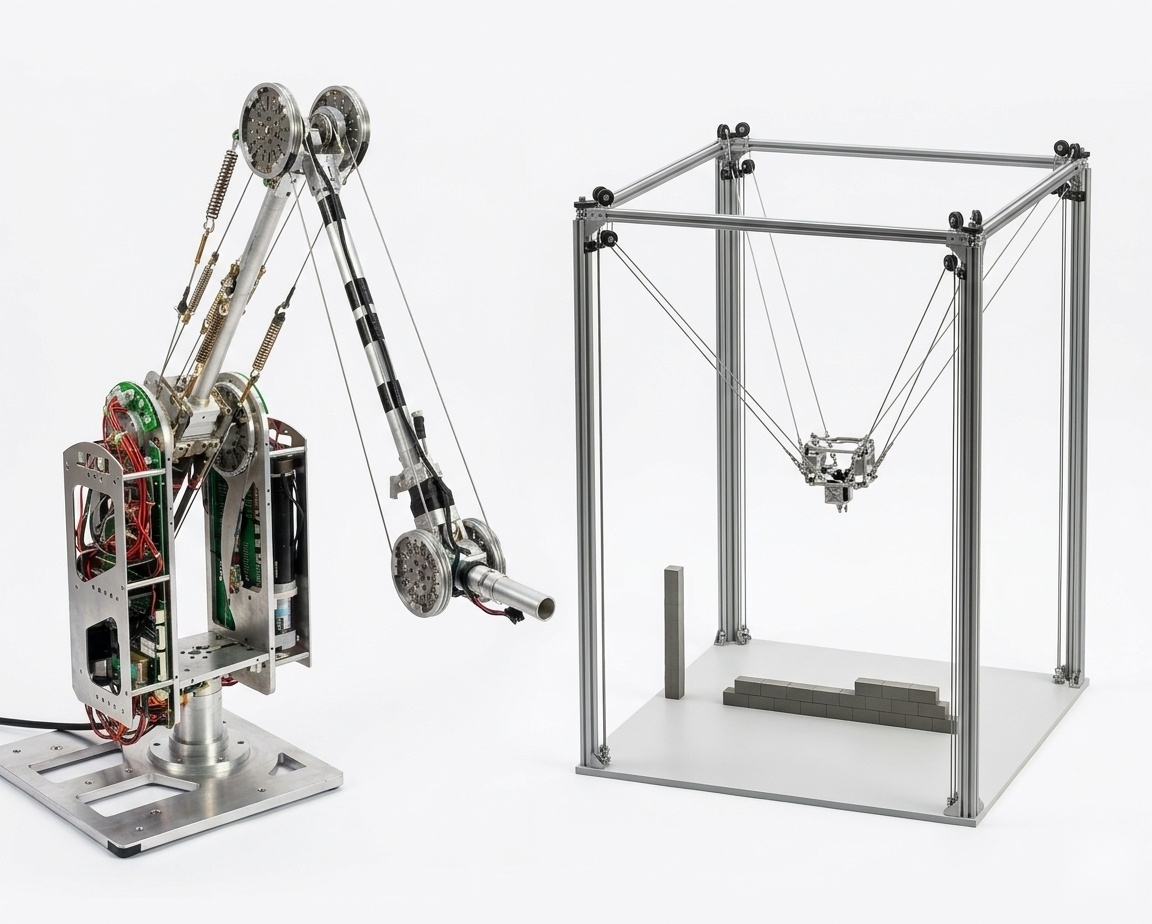
\includegraphics[width=0.88\textwidth]{robots_serie_parallele.jpg}
\caption{Robot série et robot parallèle à câble}
\label{fig:serie_parallele}
\end{figure}

\subsection{Terminologie CDPR}

Un CDPR se compose classiquement des éléments suivants :

\begin{table}[H]
\centering
\caption{Cadre théorique d'un CDPR}
\label{tab:terminologie}
\begin{tabular}{|>{\raggedright\arraybackslash}p{4.0cm}|>{\raggedright\arraybackslash}p{10.8cm}|}
\hline
\textbf{Terme} & \textbf{Définition} \\
\hline
Structure porteuse / bâti fixe & Cadre fixe sur lequel sont montés les enrouleurs. \\
\hline
Enrouleur & Dispositif motorisé qui enroule ou déroule le câble pour en faire varier la longueur active. \\
\hline
Point d'ancrage & Point, côté bâti ou côté plateforme, où le câble est guidé ou fixé. \\
\hline
Plateforme mobile (PM) & Organe terminal suspendu par les câbles, dont la pose est déterminée par le contrôle coordonné des longueurs de câble. \\
\hline
Reconfigurable & Capacité à modifier la géométrie du robot en déplaçant les points d'ancrage, sans changer la structure porteuse. \\
\hline
Degré de liberté (DDL) & Nombre de paramètres indépendants nécessaires pour décrire la pose de la plateforme (jusqu'à 6 en 3D : 3 translations + 3 rotations). \\
\hline
\end{tabular}
\end{table}

\begin{figure}[H]
\centering
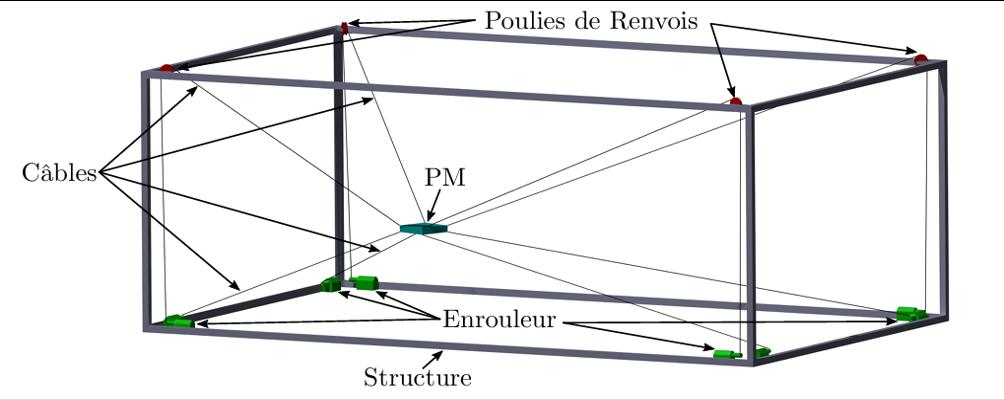
\includegraphics[width=0.92\textwidth]{cdpr_annote.png}
\caption{Schéma annoté d'un CDPR}
\label{fig:cdpr}
\end{figure}

\subsection{Classification cinématique}

Le critère de classification le plus fondamental des CDPR compare le nombre de câbles actifs \( m \) au nombre de degrés de liberté \( n \) de la plateforme :

\begin{itemize}[itemsep=3pt]
  \item \textbf{Sous-contraint} (\( m < n+1 \)) : les câbles ne suffisent pas à contraindre tous les mouvements possibles ; l'équilibre nécessite l'aide de la gravité ou d'une force extérieure.
  \item \textbf{Totalement contraint} (\( m = n+1 \)) : les câbles suffisent tout juste à contraindre tous les degrés de liberté.
  \item \textbf{Sur-contraint / redondant} (\( m > n+1 \)) : le nombre de câbles dépasse le strict nécessaire, ce qui améliore la capacité à générer des efforts dans toutes les directions, mais impose de répartir la tension entre câbles, car plusieurs répartitions sont possibles pour une même pose.
\end{itemize}

Une seconde classification distingue les CDPR selon la disposition des câbles par rapport à la plateforme :

\begin{itemize}[itemsep=3pt]
  \item \textbf{Architecture suspendue} : tous les câbles sont positionnés au-dessus de la plateforme ; la gravité maintient les câbles en tension. L'espace sous la plateforme reste dégagé, ce qui favorise un grand espace de travail, au prix d'un fonctionnement plutôt statique.
  \item \textbf{Architecture à câbles antagonistes} : les câbles sont répartis de part et d'autre de la plateforme et tirent les uns contre les autres, garantissant des tensions positives indépendamment de la gravité, ce qui permet des mouvements plus dynamiques.
\end{itemize}

\section{Modèles géométriques}

\subsection{Modèle géométrique inverse (MGI)}

Le MGI répond à une question simple : quelle longueur de câble faut-il pour amener la plateforme dans une pose donnée ? Pour un robot à câbles, ce problème se ramène en réalité à un calcul de distance entre deux points, ce qui en fait le plus facile à résoudre des trois modèles.

Notons $m$ le nombre de câbles, $(\mathbf{a}_i)$ le point d'ancrage fixe du câble $i$ sur le bâti, $(\mathbf{b}_i)$ son point d'attache sur la plateforme (exprimé dans le repère corps), $(\mathbf{p} = [x,y,z]^T)$ la position du centre de la plateforme dans le repère monde, et $(\mathbf{R})$ la matrice de rotation associée. Le vecteur reliant l'attache à l'ancrage s'écrit :
\begin{equation}
\mathbf{q}_i = \mathbf{a}_i - \mathbf{p} - \mathbf{R}\mathbf{b}_i
\label{eq:qi}
\end{equation}
D'où la longueur du câble $i$, simple norme de ce vecteur :
\begin{equation}
l_i = \|\mathbf{q}_i\| = \|\mathbf{a}_i - \mathbf{p} - \mathbf{R}\mathbf{b}_i\|
\label{eq:li}
\end{equation}

\paragraph{Translation et rotation autour de Z.}
Dans cette configuration, la plateforme possède quatre degrés de liberté : les trois translations $(x, y, z)$ et une rotation $(\varphi)$ autour de l'axe vertical. La matrice de rotation prend la forme :
\begin{equation}
\mathbf{R}(\varphi) = \begin{pmatrix}
\cos\varphi & -\sin\varphi & 0 \\
\sin\varphi & \cos\varphi & 0 \\
0 & 0 & 1
\end{pmatrix}
\label{eq:Rphi}
\end{equation}
Pour un point d'attache $(\mathbf{b}_i = [b_{ix}, b_{iy}, b_{iz}]^T)$, on obtient :
\begin{equation}
\mathbf{R}(\varphi)\mathbf{b}_i = \begin{pmatrix}
b_{ix}\cos\varphi - b_{iy}\sin\varphi \\
b_{ix}\sin\varphi + b_{iy}\cos\varphi \\
b_{iz}
\end{pmatrix}
\end{equation}
d'où la longueur de câble explicite :
\begin{equation}
\begin{aligned}
l_i = \Big( &(a_{ix}-x-b_{ix}\cos\varphi+b_{iy}\sin\varphi)^2 \\
&+ (a_{iy}-y-b_{ix}\sin\varphi-b_{iy}\cos\varphi)^2 \\
&+ (a_{iz}-z-b_{iz})^2 \Big)^{1/2}
\end{aligned}
\label{eq:li_schoenflies}
\end{equation}
On retrouve cette formulation chez Wang et al. (2022), appliquée aux robots suspendus animés de mouvements de Schönflies \cite{mdpi2022}.

\paragraph{Translation pure.}
Sans rotation $(\varphi = 0)$, la matrice de rotation se réduit à l'identité et l'expression se simplifie nettement :
\begin{equation}
l_i = \sqrt{(a_{ix}-x-b_{ix})^2 + (a_{iy}-y-b_{iy})^2 + (a_{iz}-z-b_{iz})^2}
\label{eq:li_pure}
\end{equation}
Cette forme, ne faisant intervenir que des opérations élémentaires, se prête bien au contrôle en temps réel.

\subsection{Modèle géométrique direct (MGD)}

À l'inverse du MGI, le MGD part des longueurs de câbles mesurées $(l_i)$ pour retrouver la pose $((x,y,z,\varphi))$ de la plateforme. Le problème devient alors non linéaire, et peut admettre plusieurs solutions. Il s'écrit de façon générale :
\begin{equation}
\|\mathbf{a}_i - \mathbf{p} - \mathbf{R}\mathbf{b}_i\|^2 = l_i^2, \quad i = 1, \dots, m
\label{eq:mgd}
\end{equation}

\paragraph{Translation et rotation autour de Z.}
En explicitant la rotation, on obtient le système :
\begin{equation}
\begin{cases}
(a_{ix}-x-b_{ix}\cos\varphi+b_{iy}\sin\varphi)^2 \\
+(a_{iy}-y-b_{ix}\sin\varphi-b_{iy}\cos\varphi)^2 \\
+(a_{iz}-z-b_{iz})^2 = l_i^2
\end{cases}
\qquad i = 1, \dots, m
\end{equation}
Avec $(m = 4)$, on a autant d'équations que d'inconnues. Une résolution analytique reste possible dans certains cas particuliers : c'est l'approche par projection plane proposée par Wang et al. (2022) \cite{mdpi2022} : mais on recourt le plus souvent à une méthode numérique de type Newton-Raphson. Plus récemment, Zhang et al. (2024) ont proposé, avec CafkNet, une alternative fondée sur des réseaux de neurones sur graphes, utile quand la géométrie devient trop complexe pour une résolution classique \cite{zhang2024}.

\paragraph{Translation pure.}
Avec $(\varphi = 0)$, le système se réduit à :
\begin{equation}
(a_{ix}-x-b_{ix})^2 + (a_{iy}-y-b_{iy})^2 + (a_{iz}-z-b_{iz})^2 = l_i^2
\end{equation}
Ce qui revient géométriquement à chercher l'intersection de sphères centrées sur les points d'ancrage. Le problème demeure non linéaire, mais reste plus abordable que dans le cas avec rotation.

\subsection{Matrice de structure (Jacobienne)}

La matrice de structure $(\mathbf{J})$ relie les vitesses de la plateforme aux vitesses de déroulement des câbles. Elle joue un rôle central dans l'analyse dynamique comme dans la commande du robot.

Pour chaque câble $i$, on définit le vecteur unitaire $(\mathbf{u}_i = \mathbf{q}_i / l_i)$, orienté de la plateforme vers le bâti. La vitesse de déroulement s'écrit alors :
\begin{equation}
\dot{l}_i = -\mathbf{u}_i^T\dot{\mathbf{p}} - (\mathbf{r}_i \times \mathbf{u}_i)^T \boldsymbol{\omega}
\label{eq:ldot}
\end{equation}
avec $(\mathbf{r}_i = \mathbf{R}\mathbf{b}_i)$ et $(\boldsymbol{\omega})$ le vecteur vitesse angulaire, ce qui permet d'écrire $(\dot{\mathbf{l}} = \mathbf{J}\dot{\mathbf{X}})$, où $(\dot{\mathbf{X}} = [\dot{\mathbf{p}}^T, \boldsymbol{\omega}^T]^T)$. Cette matrice est explicitée par Wang et al. (2022) \cite{mdpi2022}, et exploitée par Cheah et al. (2022) pour la distribution des tensions \cite{arXiv2403}.

\paragraph{Translation et rotation autour de Z.}
La vitesse angulaire se réduit ici à $(\boldsymbol{\omega} = [0, 0, \dot{\varphi}]^T)$, et la ligne $i$ de la jacobienne devient :
\begin{equation}
\mathbf{J}_i = \begin{bmatrix} -u_{ix} & -u_{iy} & -u_{iz} & -\mathbf{u}_i^T \mathbf{R}'(\varphi)\mathbf{b}_i \end{bmatrix}
\end{equation}
Avec
\begin{equation}
\mathbf{R}'(\varphi)\mathbf{b}_i = \begin{pmatrix}
-b_{ix}\sin\varphi - b_{iy}\cos\varphi \\
b_{ix}\cos\varphi - b_{iy}\sin\varphi \\
0
\end{pmatrix}
\end{equation}
La matrice complète $(\mathbf{J} \in \mathbb{R}^{m \times 4})$ s'obtient en empilant ces lignes.

\paragraph{Translation pure.}
Sans rotation, le terme en $\varphi$ disparaît simplement, et la matrice se réduit à :
\begin{equation}
\mathbf{J}_i = \begin{bmatrix} -u_{ix} & -u_{iy} & -u_{iz} \end{bmatrix}, \qquad \mathbf{J} \in \mathbb{R}^{m \times 3}
\end{equation}
Une forme particulièrement pratique pour les déplacements plans ou les mouvements de balayage à orientation fixe.

\paragraph{Cas général 6-DDL et distinction cinématique / statique.}
Dans le cas général d'un robot spatial à 6 degrés de liberté (3 translations + 3 rotations), la matrice de structure est de dimension $6 \times m$. Chaque colonne $i$ contient le torseur unitaire du câble $i$ :
\begin{equation}
\mathbf{W}_i = \begin{bmatrix} \mathbf{u}_i \\ \mathbf{r}_i \times \mathbf{u}_i \end{bmatrix} \in \mathbb{R}^6
\label{eq:Wi}
\end{equation}
où $\mathbf{u}_i$ est le vecteur unitaire du câble et $\mathbf{r}_i \times \mathbf{u}_i$ le moment associé.

Il convient de distinguer deux usages de cette matrice :
\begin{itemize}
\item \textbf{Cinématique de la trajectoire} : lorsque le robot est planifié en translation pure (orientation fixe $\mathbf{R} = I$), la matrice $\mathbf{J} \in \mathbb{R}^{m \times 3}$ suffit pour calculer les longueurs de câbles et les vitesses de déroulement le long de la trajectoire.
\item \textbf{Équilibre statique et faisabilité en tension} : pour garantir que la plateforme ne subit aucun moment résiduel (même en translation pure, les câbles exercent des moments), l'équilibre statique est vérifié en 6-DDL avec la matrice $\mathbf{W} \in \mathbb{R}^{6 \times m}$ (3 forces + 3 moments). C'est cette matrice qui est utilisée pour le test de faisabilité en tension (WFW, section 1.5.4).
\end{itemize}

Enfin, l'équilibre statique de la plateforme s'exprime par :
\begin{equation}
\mathbf{W}^T \mathbf{f} = -\mathbf{w}_{\mathrm{ext}}, \qquad f_i \geq 0, \qquad f_{\min} \leq f_i \leq f_{\max}
\label{eq:equilibre_statique}
\end{equation}
$\mathbf{f}$ désignant le vecteur des tensions de câble et $\mathbf{w}_{\mathrm{ext}}$ le torseur des efforts extérieurs. Dès lors que le système est redondant ($m > n$), il existe une infinité de distributions de tensions possibles : une marge de manœuvre précieuse pour l'optimisation \cite{tho2022}, \cite{arXiv2403}.

\section{Modèles de câble}

Le choix du modèle de câble conditionne directement la précision et la validité des simulations d'un robot parallèle à câbles (CDPR). Selon l'échelle du robot, la masse des câbles, le niveau de tension appliqué et la précision recherchée, plusieurs niveaux de modélisation sont envisageables. La littérature en distingue classiquement trois : le câble rigide, le câble élastique et le câble caténaire \cite{tho2022}. La figure ci-dessous en résume le principe.

\begin{figure}[H]
\centering
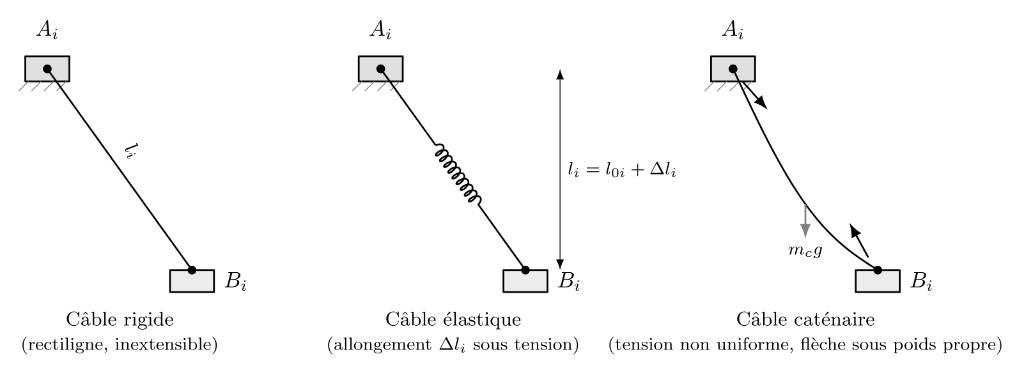
\includegraphics[width=0.95\textwidth]{cable_models.jpg}
\caption{Les trois modèles de câble : rigide, élastique, caténaire}
\label{fig:modeles_cable}
\end{figure}

\subsection{Câble rigide}

Le modèle de câble rigide est le plus simple. Il repose sur trois hypothèses :
\begin{itemize}
\item Le câble est sans masse ;
\item Il est inextensible, c'est-à-dire de raideur infinie ;
\item Il reste rectiligne entre ses deux points d'attache.
\end{itemize}
Dans ce modèle, la longueur du câble est directement donnée par la distance euclidienne entre le point d'ancrage fixe $A_i$ et le point d'attache mobile $B_i$ : aucune déformation ni affaissement n'est pris en compte. Ce modèle convient bien aux robots de petite taille dont les câbles sont courts et légers, et lorsque les tensions restent suffisamment élevées pour que l'élasticité et le poids propre soient négligeables. C'est aussi le modèle le plus utilisé pour la commande en temps réel, car il conduit à des calculs rapides et simples. C'est d'ailleurs celui adopté dans le modèle géométrique inverse de la section 1.2.

\subsection{Câble élastique}

Le modèle de câble élastique introduit la raideur axiale du câble. Il suppose que le câble reste rectiligne mais s'allonge proportionnellement à la tension appliquée, selon la loi de Hooke :
\begin{equation}
f_i = k_i (l_i - l_{0i})
\label{eq:hooke}
\end{equation}
où $l_i$ est la longueur actuelle du câble, $l_{0i}$ sa longueur à vide, et $k_i$ sa raideur axiale, donnée par :
\begin{equation}
k_i = \frac{E A}{l_{0i}}
\label{eq:ki}
\end{equation}
Avec $E$ : le module d'Young du matériau et $A$ la section du câble. Ce modèle est plus réaliste que le précédent dès lors que les câbles sont plus longs ou les charges plus importantes : il permet de prendre en compte l'allongement du câble sous tension, ce qui améliore la précision du positionnement. Il néglige en revanche toujours l'affaissement dû au poids propre du câble.

\subsection{Câble caténaire}

Le modèle de câble caténaire, le plus complet des trois, considère que le câble prend, sous l'effet de son propre poids, la forme d'une courbe caténaire entre ses deux points d'attache. La tension n'est alors plus uniforme le long du câble. Ce modèle se traduit par des équations non linéaires qui nécessitent une résolution numérique. Il devient indispensable pour les robots de grande envergure à câbles très longs, comme les robots FAST ou CoGiRo \cite{tho2022}, où l'affaissement n'est plus négligeable et affecte directement la précision de la pose. Pour de petites dimensions en revanche, son coût de calcul est généralement injustifié.

\section{Contraintes de tension}

La commande et la planification de trajectoire d'un robot parallèle à câbles (CDPR) sont conditionnées par le comportement mécanique des câbles eux-mêmes. Contrairement aux actionneurs rigides d'un robot série classique, un câble ne peut transmettre qu'un effort de traction. Cette spécificité impose deux contraintes qui doivent être respectées à tout instant et en tout point de la trajectoire : l'unilatéralité et les bornes de tension.

\subsection{Unilatéralité du câble}

Un câble ne peut exercer qu'un effort de traction ; il est incapable de pousser. La tension $f_i$ dans chacun des câbles doit donc rester strictement positive à tout instant :
\begin{equation}
f_i > 0 \qquad \text{(ou plus pratiquement } f_i \ge f_{\min}\text{)}
\label{eq:unilateralite}
\end{equation}
Cette contrainte, dite d'unilatéralité, constitue la condition fondamentale de faisabilité d'un CDPR \cite{tho2022}. Si la tension d'un câble s'annule, il se détend : la plateforme perd alors sa rigidité et le contrôle de sa pose n'est plus assuré, ce qui peut conduire à des oscillations, des imprécisions de positionnement, voire une instabilité du système.

En pratique, on n'exige pas seulement $f_i > 0$, mais $f_i \ge f_{\min}$, où $f_{\min}$ est une tension minimale de sécurité qui garantit que le câble reste tendu malgré les perturbations (vent, vibrations, imprécisions de mesure).

\subsection{Bornes de tension}

Si l'unilatéralité impose une borne inférieure, la résistance mécanique des câbles et la capacité des actionneurs imposent une borne supérieure. La tension dans chaque câble doit donc respecter l'intervalle suivant :
\begin{equation}
f_{\min} \le f_i \le f_{\max}
\label{eq:bornes}
\end{equation}
La borne inférieure $f_{\min}$ est fixée par la nécessité de maintenir tous les câbles tendus. Elle dépend de la précontrainte initiale, de la masse de la plateforme et des perturbations externes attendues.

La borne supérieure $f_{\max}$ est quant à elle déterminée par trois facteurs :
\begin{itemize}
\item La charge de rupture du câble, divisée par un facteur de sécurité ;
\item La capacité maximale des moteurs et des réducteurs, qui ne peuvent fournir qu'un couple limité ;
\item La déformation acceptable de la structure, le bâti ne devant pas fléchir sous l'effort.
\end{itemize}

Le respect simultané de ces bornes définit ce que la littérature appelle l'espace de travail en tension : l'ensemble des poses pour lesquelles il existe une distribution de tensions satisfaisant $f_{\min} \leq f_i \leq f_{\max}$ \cite{tho2022}.

Pour la planification : une trajectoire n'est réalisable que si, à chaque instant, les tensions calculées par la dynamique inverse restent dans l'intervalle admissible. Le non-respect de cette contrainte invalide la trajectoire, même si elle respecte par ailleurs les limites cinématiques des moteurs (vitesse, accélération).

\section{Espaces de travail}

La notion d'espace de travail est plus restrictive dans un robot parallèle à câbles que pour un robot rigide classique. En raison de l'unilatéralité des câbles et des bornes de tension, toutes les poses géométriquement atteignables ne sont pas nécessairement contrôlables. Duan et al. proposent une classification des espaces de travail fondée sur l'équation générale du mouvement et la propriété unilatérale des câbles \cite{duan2014}. Cette classification distingue cinq types d'espaces, dont trois sont particulièrement pertinents pour la planification de trajectoire.

\subsection{Espace de travail géométrique}

L'espace de travail géométrique est le plus large des espaces considérés. Il correspond à l'ensemble des poses pour lesquelles les longueurs de câbles calculées par le MGI (section 1.2) restent comprises entre les longueurs minimale et maximale admissibles, un câble ni totalement enroulé, ni totalement déroulé. Cet espace ne tient compte ni des tensions, ni de la gravité, ni de la capacité des moteurs : il fournit simplement une borne supérieure de l'espace réellement exploitable.

\subsection{Espace d'équilibre statique (SEW)}

L'espace d'équilibre statique (Static Equilibrium Workspace, SEW) est le sous-ensemble de l'espace géométrique dans lequel la plateforme peut être maintenue à l'arrêt, sous l'effet de la gravité, avec toutes les tensions positives \cite{duan2014}. Formellement, il existe un vecteur de tensions $\mathbf{f} > 0$ tel que :
\begin{equation}
\mathbf{J}^T \mathbf{f} + \mathbf{w}_g = \mathbf{0}
\label{eq:sew}
\end{equation}
où $\mathbf{J}^T$ est la matrice de structure transposée (section 1.2) et $\mathbf{w}_g$ le torseur de gravité. Le SEW est donc l'ensemble des poses où le robot peut tenir sa position sans bouger, mais il ne préjuge en rien de sa capacité à résister à des efforts externes.

\subsection{Espace de fermeture en effort (WCW)}

L'espace de fermeture en effort (Wrench Closure Workspace, WCW) est l'ensemble des poses pour lesquelles la plateforme peut équilibrer n'importe quel torseur d'effort : force et moment appliqué de l'extérieur, en tirant uniquement sur les câbles \cite{duan2014}. Autrement dit, quelle que soit la perturbation, il existe une distribution de tensions positives capable de la contrer. Le WCW est un espace très restrictif : il n'existe que pour les robots complètement contraints (au moins $n+1$ câbles pour $n$ degrés de liberté), et suppose qu'il n'y a aucune limite supérieure sur les tensions.

\subsection{Espace faisable en effort (WFW)}

L'espace faisable en effort (Wrench-Feasible Workspace, WFW) est le concept le plus pertinent pour la planification de trajectoire. Il correspond à l'ensemble des poses pour lesquelles la plateforme peut équilibrer un ensemble de torseurs d'effort prescrits, tout en gardant les tensions dans un intervalle borné :
\begin{equation}
f_{\min} \le f_i \le f_{\max}, \qquad \forall i \in \{1, \dots, m\}
\label{eq:wfw}
\end{equation}
Contrairement au WCW, le WFW prend en compte :
\begin{itemize}
\item La limite supérieure des tensions, liée à la capacité des moteurs et à la résistance des câbles ;
\item La limite inférieure, nécessaire au maintien de la tension pour éviter le mou (unilatéralité en section 1.4).
\end{itemize}
Le WFW constitue donc l'espace de travail réellement exploitable pour un CDPR. Une trajectoire n'est réalisable que si elle reste intégralement incluse dans le WFW. Son calcul dépend de la géométrie du robot, des bornes de tension et de l'ensemble des perturbations à contrer \cite{duan2014}.

Le tableau ci-dessous résume la hiérarchie des espaces de travail, du plus large au plus restrictif :

\begin{table}[H]
\centering
\caption{Synthèse comparative des espaces de travail}
\label{tab:espaces}
\resizebox{\textwidth}{!}{%
\begin{tabular}{|l|>{\raggedright\arraybackslash}p{3.6cm}|>{\raggedright\arraybackslash}p{3.0cm}|c|>{\raggedright\arraybackslash}p{3.0cm}|}
\hline
\textbf{Type d'espace} & \textbf{Condition} & \textbf{Limite de tension} & \textbf{Gravité} & \textbf{Utilisation} \\
\hline
Géométrique & Longueurs de câbles valides & Aucune & Non & Borne supérieure \\
\hline
SEW & $\mathbf{f} > 0$, équilibre statique & $f_i > 0$ & Oui & Pose de repos \\
\hline
WCW & Torseur quelconque équilibrable & $f_i > 0$ & Oui & Robots complètement contraints \\
\hline
WFW & Torseur prescrit équilibrable & $f_{\min} \leq f_i \leq f_{\max}$ & Oui & Planification de trajectoire \\
\hline
\end{tabular}%
}
\end{table}

\section*{Conclusion}

Ce chapitre a montré que la spécificité du CDPR, des câbles qui ne peuvent que tirer, impose des contraintes propres qui définissent en dernier ressort l'espace de travail réellement exploitable, le WFW. Cet espace, associé au modèle géométrique et à la représentation retenue de l'environnement, constitue désormais le cadre dans lequel toute trajectoire du robot Tandem devra s'inscrire. Il reste cependant à déterminer comment générer, à l'intérieur de ce cadre, un chemin couvrant la parcelle tout en conciliant rapidité, économie d'énergie et précision des prises de vue. C'est l'objet du chapitre suivant, consacré aux méthodes de planification et d'optimisation de trajectoire.

% ============================================================
% CHAPITRE 2 (début)
% ============================================================

\chapter{PLANIFICATION DES TRAJECTOIRES}

\section{Path and trajectory planning}

\subsection{Définitions}

Le \textbf{path planning} (planification de chemin) consiste à déterminer un \textbf{chemin géométrique} reliant un point initial à un point final, en passant éventuellement par des points de passage intermédiaires (\textit{via-points}). Ce chemin est une courbe purement spatiale, définie dans l'espace articulaire ou dans l'espace opérationnel du robot. Il s'agit de savoir « par où passe le robot » sans aucune référence au temps, à la vitesse ou à l'accélération \cite{gasparetto2015}.

Le \textbf{trajectory planning} (planification de trajectoire) prend ce chemin géométrique comme donnée d'entrée et y \textbf{associe une information temporelle} : à quel instant le robot doit se trouver à chaque point du chemin, avec quelle vitesse et quelle accélération \cite{gasparetto2015}.

Elle conditionne directement la qualité du mouvement : le choix des temps de passage aux \textit{via-points} influence non seulement les propriétés \textbf{cinématiques} du mouvement (vitesse, accélération), mais aussi ses propriétés \textbf{dynamiques}, les efforts inertiels subis par le robot dépendent des accélérations, et les vibrations de sa structure mécanique sont déterminées par les valeurs du \textbf{jerk} (dérivée de l'accélération) \cite{gasparetto2015}.

\begin{figure}[H]
\centering
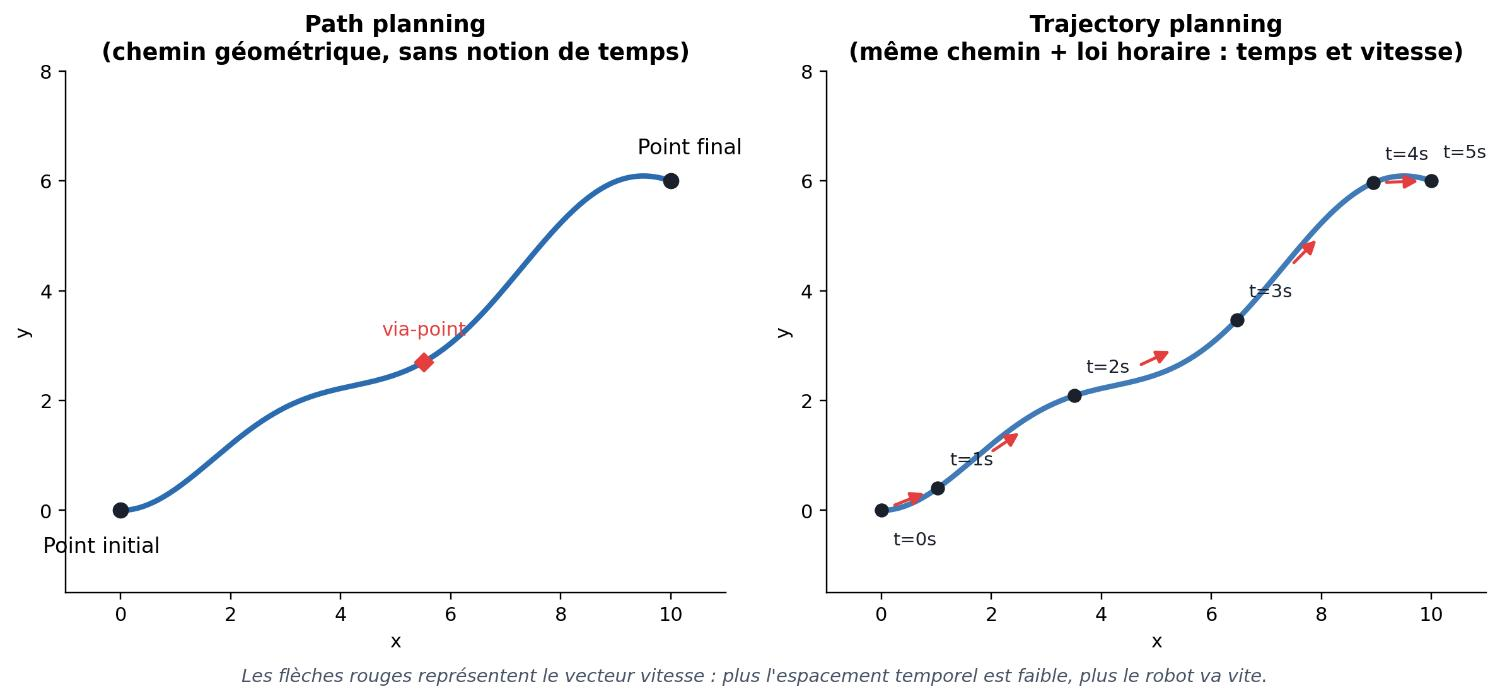
\includegraphics[width=0.88\textwidth]{path_vs_trajectory.png}
\caption{Comparaison chemin vs trajectoire}
\label{fig:path_vs_traj}
\end{figure}

\subsection{Faisabilité cinématique et dynamique}

La séparation entre path et trajectory planning permet de traiter la faisabilité du mouvement à deux niveaux complémentaires.

\textbf{Au niveau du path planning}, c'est purement géométrique : le chemin existe-t-il, et est-il admissible ? Cela implique de vérifier que le chemin ne traverse pas d'obstacles, qu'il respecte les limites de l'espace de travail, et qu'il est compatible avec la cinématique du mécanisme.

\textbf{Au niveau du trajectory planning}, cela devient temporelle et dynamique : le robot peut-il parcourir ce chemin dans les temps, sans dépasser les limites de vitesse et d'accélération de ses actionneurs, sans générer de vibrations excessives, et sans violer les contraintes dynamiques du système ? Les algorithmes de planification de trajectoire sont classiquement nommés selon la fonction qu'ils optimisent : \textbf{temps minimal}, \textbf{énergie minimale} ou \textbf{jerk minimal} \cite{gasparetto2015}.

\section{Génération de chemin}

La génération de chemin consiste à déterminer la courbe géométrique que le robot doit suivre, indépendamment de la considération temporelle. Selon la nature de la mission, deux grandes familles de problèmes se distinguent : la \textbf{couverture complète} d'une zone (Coverage Path Planning, CPP), où le robot doit passer par tous les points d'une région, et la \textbf{tournée de points discrets} (TSP, VRP), où il s'agit de visiter un ensemble fini de cibles selon un ordre. À ces deux familles s'ajoutent les algorithmes de recherche sur graphe ou par échantillonnage, mobilisés lorsque l'environnement est encombré d'obstacles \cite{gasparetto2015}.

\subsection{Couverture complète (CPP)}

La planification de chemin pour couverture complète a pour objectif de générer un chemin passant par \textbf{tous les points} d'une zone, sans distinction. Ce problème se rencontre dans plusieurs applications : nettoyage robotisé, cartographie, surveillance agricole, inspection de surfaces \cite{choset1998}.

\begin{figure}[H]
\centering
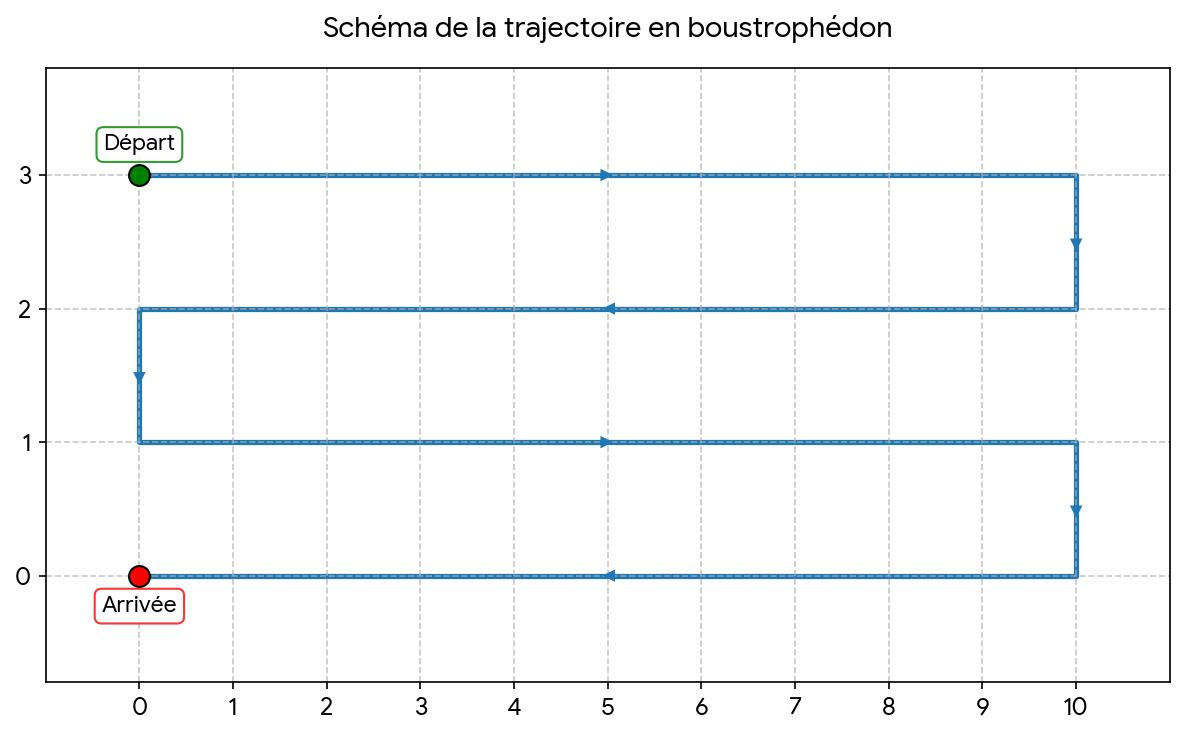
\includegraphics[width=0.85\textwidth]{boustrophedon.png}
\caption{Balayage boustrophédon}
\label{fig:boustrophedon}
\end{figure}

La méthode la plus établie demeure la \textbf{décomposition cellulaire boustrophédon} (Boustrophedon Cellular Decomposition, BCD), introduite par Choset et Pignon \cite{choset1998}. Son principe consiste à découper la zone à couvrir en \textbf{cellules convexes}, à l'aide de lignes verticales passant par les sommets des obstacles. Chaque cellule est ensuite balayée par des mouvements de va-et-vient parallèles d'où le terme « boustrophédon », qui désigne le mouvement du bœuf labourant un champ en effectuant des allers-retours successifs. Les cellules sont enfin reliées entre elles par un graphe d'adjacence, et un algorithme de parcours détermine l'ordre de visite optimal \cite{choset1998}.

\begin{figure}[H]
\centering
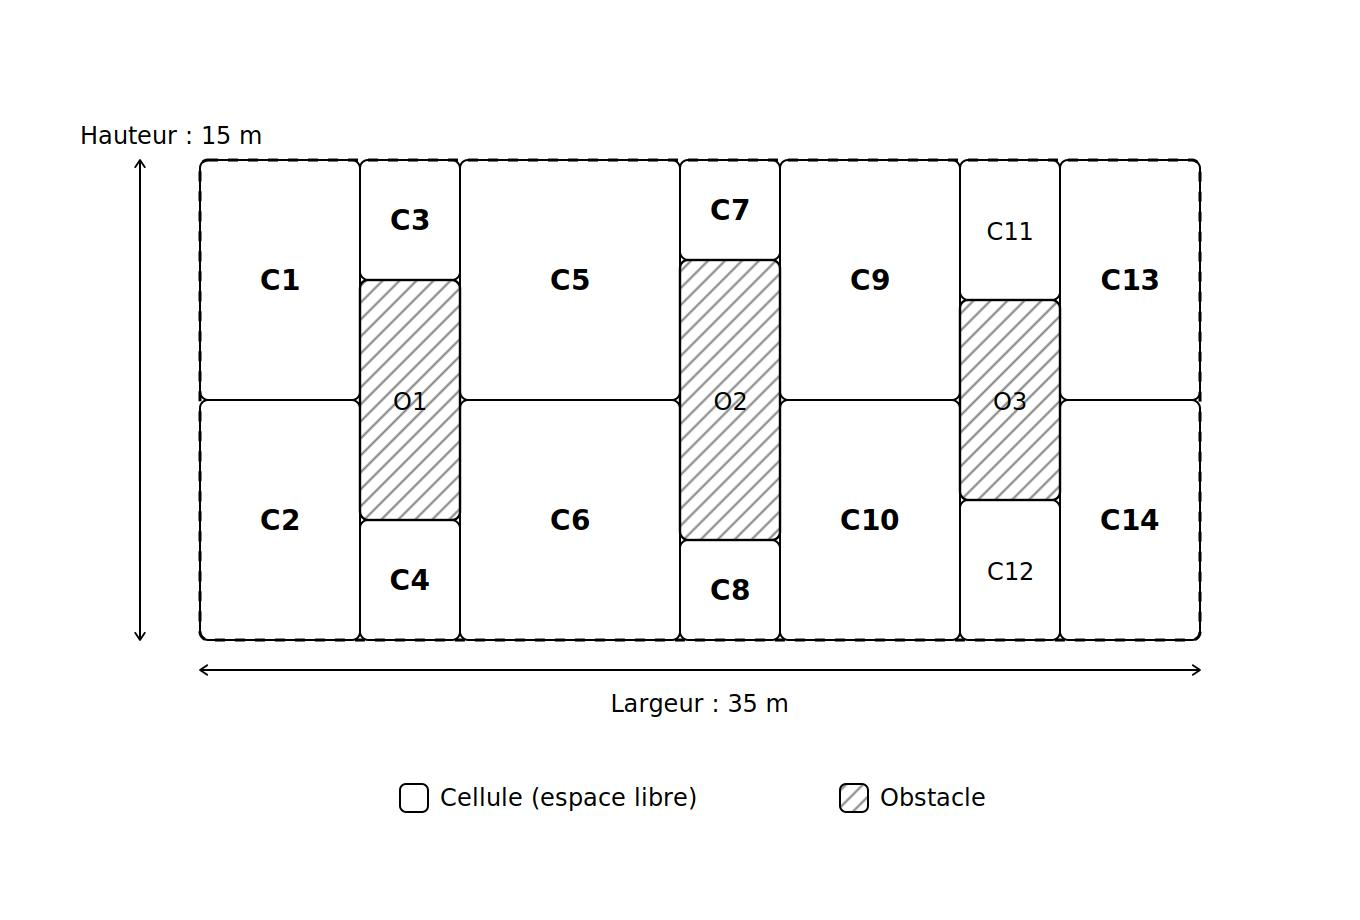
\includegraphics[width=0.90\textwidth]{decomposition_cellulaire.png}
\caption{Décomposition cellulaire (BCD)}
\label{fig:decomp_cell}
\end{figure}

Cette méthode garantit une couverture \textbf{complète} et \textbf{sans recouvrement inutile}, à condition que la zone soit plane et que les obstacles soient connus. Elle est particulièrement adaptée aux environnements structurés et de grande taille, tels que les parcelles agricoles \cite{choset1998}.

D'autres approches existent, comme les \textbf{trajectoires en spirale}, adaptées aux zones sans obstacle, et les \textbf{méthodes par champs de potentiel}. Le choix de la méthode dépend de la géométrie de la zone, de la présence d'obstacles et du critère d'optimisation retenu (temps et simplicité du chemin).

\subsection{Tournée de points discrets (TSP, VRP)}

Lorsque la mission ne consiste pas à couvrir une zone continue mais à \textbf{visiter un ensemble fini de points}, le problème se ramène à une tournée. Le cas le plus élémentaire est le \textbf{problème du voyageur de commerce} (Traveling Salesman Problem, TSP), qui consiste à déterminer l'ordre de visite de $N$ points minimisant la distance totale parcourue, avec retour au point de départ \cite{gasparetto2015}.

\begin{figure}[H]
\centering
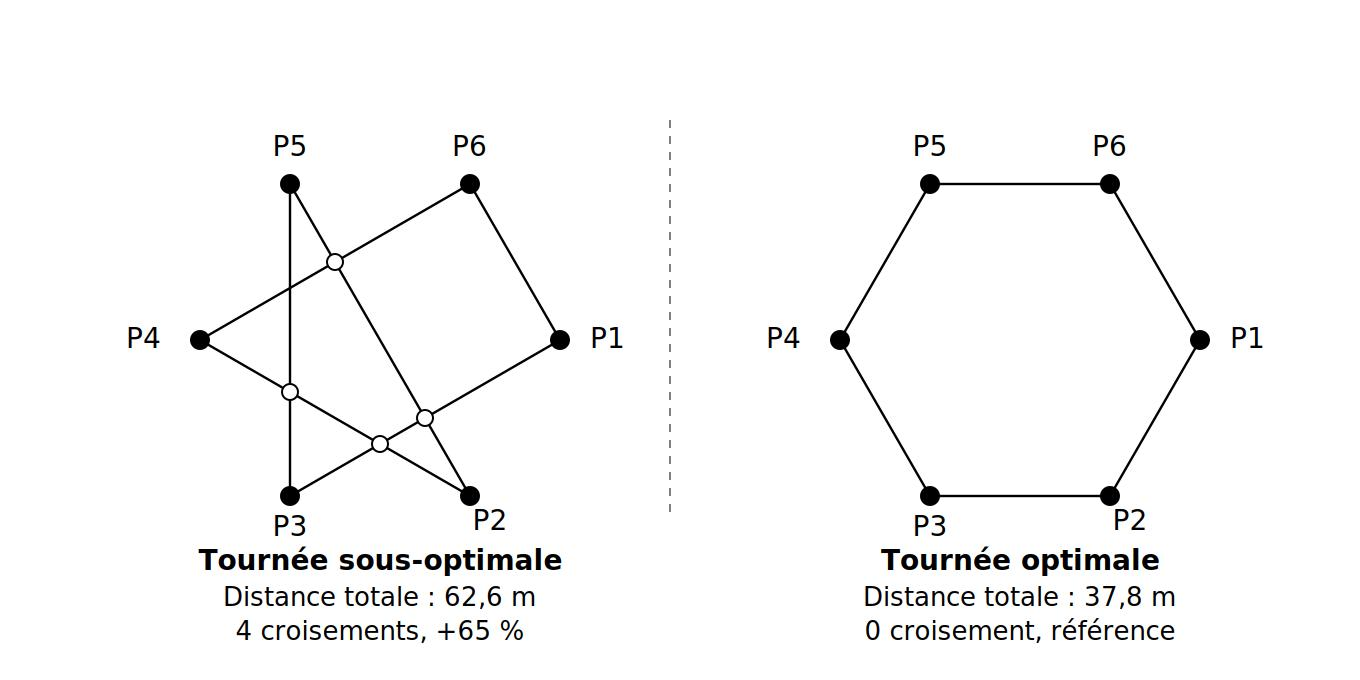
\includegraphics[width=0.88\textwidth]{tsp.png}
\caption{Tournées TSP : sous-optimale vs optimale}
\label{fig:tsp}
\end{figure}

Le TSP constitue un problème \textbf{NP-difficile} : le nombre de permutations possibles croît en $N!$, rendant toute résolution exacte impraticable au-delà d'une vingtaine de points. Pour des instances de taille supérieure, on utilise des \textbf{heuristiques} (plus proche voisin, insertion, 2-opt) ou à des \textbf{métaheuristiques} (algorithmes génétiques, recuit simulé), permettant d'obtenir des solutions proches de l'optimum dans un temps de calcul raisonnable \cite{gasparetto2015}.

Le \textbf{problème de tournée de véhicules} (Vehicle Routing Problem, VRP) constitue une généralisation du TSP à plusieurs véhicules desservant un ensemble de clients. Sa variante avec fenêtres temporelles (VRPTW) impose que chaque client soit visité dans un intervalle de temps donné. Ces problèmes, également NP-difficiles, se rencontrent en logistique et en planification de tournées \cite{gasparetto2015}.

\subsection{Algorithmes de graphe et échantillonnage}

Lorsque l'environnement est encombré d'obstacles, la génération de chemin se ramène généralement à une \textbf{recherche sur graphe}. L'espace libre est discrétisé en un ensemble de nœuds connectés par des arêtes, et un algorithme de plus court chemin détermine la séquence optimale.

Les algorithmes classiques comprennent :
\begin{itemize}
\item \textbf{Dijkstra} : détermine le plus court chemin d'un nœud source vers l'ensemble des autres nœuds, en présence de poids positifs.
\item \textbf{A*} : variante de Dijkstra guidée par une fonction heuristique, plus efficace en pratique.
\item \textbf{Floyd-Warshall} : calcule les plus courts chemins entre toutes les paires de nœuds, pour un coût de $O(n^3)$.
\end{itemize}

Ces algorithmes sont déterministes et garantissent l'optimalité, mais leur complexité dépend directement de la finesse de la discrétisation retenue. Une grille trop fine entraîne une explosion du temps de calcul ; une grille trop grossière produit des chemins en escalier \cite{gasparetto2015}.

Pour les environnements de grande dimension, les \textbf{méthodes d'échantillonnage probabiliste} sont généralement privilégiées :
\begin{itemize}
\item \textbf{RRT} (Rapidly-exploring Random Tree) : construit un arbre en explorant aléatoirement l'espace jusqu'à atteindre la cible.
\item \textbf{PRM} (Probabilistic Roadmap) : construit un graphe de routes par échantillonnage de l'espace libre, sur lequel un chemin est ensuite recherché.
\end{itemize}

\begin{figure}[H]
\centering
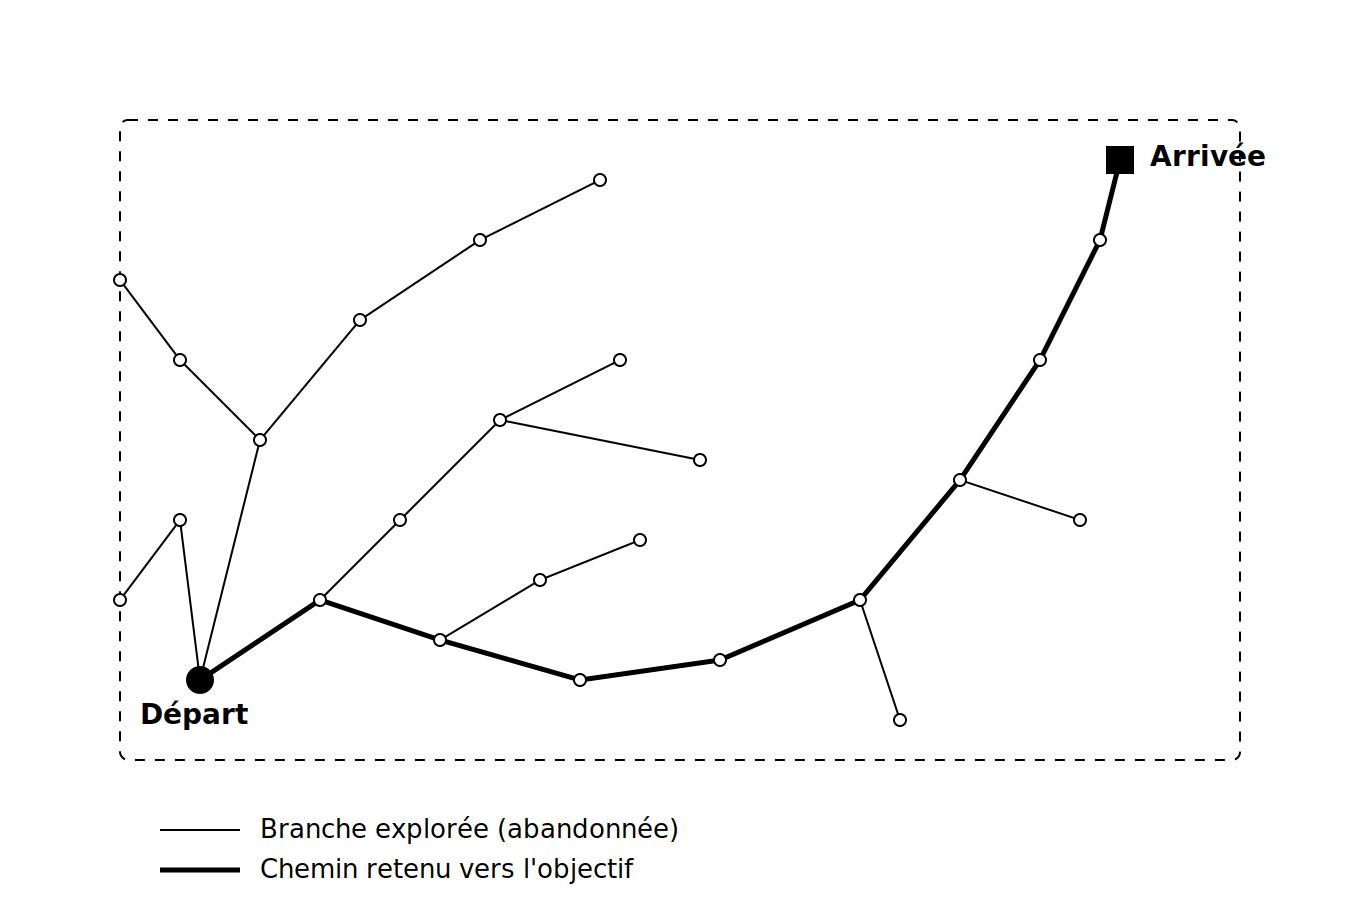
\includegraphics[width=0.80\textwidth]{rrt.png}
\caption{Principe de l'algorithme RRT}
\label{fig:rrt}
\end{figure}

Ces méthodes sont \textbf{probabilistes} : elles convergent vers une solution avec une probabilité croissante, sans garantir l'optimalité. Elles sont adaptées aux robots présentant un grand nombre de degrés de liberté, mais s'avèrent moins efficaces que les méthodes déterministes dans des espaces simples et structurés \cite{gasparetto2015}.

Le tableau ci-dessous résume les caractéristiques des principales familles de méthodes.

\begin{table}[H]
\centering
\caption{Tableau comparatif des méthodes de génération de chemin}
\label{tab:methodes_chemin}
\footnotesize
\begin{tabular}{|>{\raggedright\arraybackslash}p{2.5cm}|>{\raggedright\arraybackslash}p{2.3cm}|>{\raggedright\arraybackslash}p{2.1cm}|>{\raggedright\arraybackslash}p{2.3cm}|>{\raggedright\arraybackslash}p{2.9cm}|}
\hline
\textbf{Méthode} & \textbf{Type de problème} & \textbf{Optimalité} & \textbf{Complexité} & \textbf{Adaptée à} \\
\hline
Boustrophédon (BCD) & Couverture complète & Complète & Modérée & Zones structurées sans obstacle complexe \\
\hline
Spirale & Couverture complète & Complète & Faible & Zones convexes sans obstacle \\
\hline
TSP (exact) & Tournée de points & Optimale & $O(N!)$ explose & Très petits ensembles ($N < 20$) \\
\hline
TSP (heuristique) & Tournée de points & Proche de l'optimum & $O(N^2)$ à $O(N^3)$ & Grands ensembles \\
\hline
Dijkstra / A* & Graphe discret & Optimale & $O(n \log n)$ & Environnements discrets modérés \\
\hline
RRT / PRM & Espace continu & Probabiliste & Variable & Environnements complexes, grande dimension \\
\hline
\end{tabular}
\end{table}

\textbf{Remarque :} le choix d'une méthode dépend de la nature de la tâche (couverture ou visite de points), de la taille de l'espace considéré, de la présence d'obstacles et du compromis entre optimalité et temps de calcul. Pour une zone structurée et sans obstacle, la \textbf{décomposition boustrophédon} \cite{choset1998} constitue la méthode la plus simple et la plus robuste pour assurer une couverture complète. Pour la visite de points précis, une \textbf{heuristique de type plus proche voisin} offre un compromis satisfaisant entre qualité de solution et temps de calcul. Les algorithmes de graphe et d'échantillonnage sont réservés aux environnements encombrés ou de grande dimension \cite{gasparetto2015}.

\section{Lissage de trajectoire}

Une fois le chemin géométrique déterminé (section 2.2), il faut définir comment le robot va le parcourir dans le temps. Cette étape, appelée \textit{trajectory planning}, consiste à associer à chaque point du chemin un instant de passage, une vitesse et une accélération. Le choix de la méthode d'interpolation conditionne directement la douceur du mouvement, les sollicitations mécaniques et la qualité du suivi \cite{gasparetto2015}.

\begin{figure}[H]
\centering
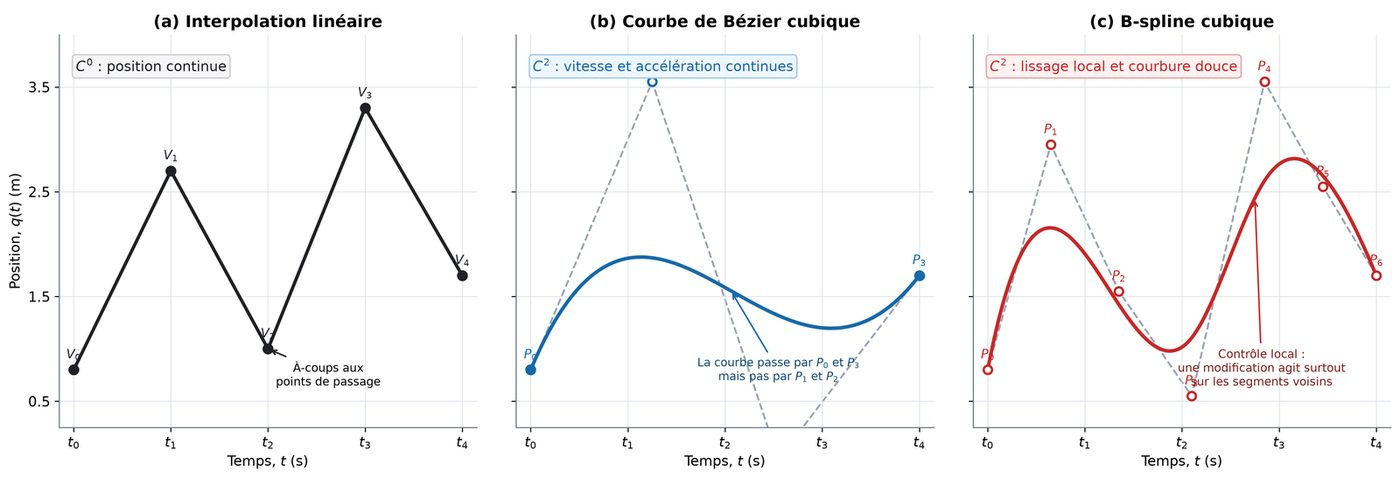
\includegraphics[width=0.98\textwidth]{lissage.jpg}
\caption{Comparaison des méthodes de lissage}
\label{fig:lissage}
\end{figure}

\begin{itemize}
\item La méthode la plus simple consiste à relier les points de passage par des \textbf{segments de droite}, en imposant une vitesse constante sur chaque segment. Cette approche, dite \textbf{interpolation linéaire}, est simple à mettre en œuvre.

Cependant, elle possède \textbf{deux limites majeures} \cite{gasparetto2015} :
\begin{itemize}
\item \textbf{Discontinuité de vitesse aux points de passage.} Lorsque le robot change de segment, sa vitesse passe brutalement d'une valeur à une autre, ce qui se traduit par un \textbf{à-coup} mécanique. Cette discontinuité est de classe $C^0$ (continuité de position seulement), insuffisante pour un mouvement fluide.
\item \textbf{Discontinuité d'accélération.} Aux extrémités de chaque segment, l'accélération est théoriquement infinie. En pratique, cela se traduit par des pics de couple sur les actionneurs, des vibrations et une usure prématurée de la mécanique.
\end{itemize}

Ces défauts sont particulièrement pénalisants pour les robots à structure flexible, comme les robots à câbles, où les à-coups provoquent les modes vibratoires et dégradent la précision. Pour obtenir un mouvement fluide, il faut donc utiliser des \textbf{courbes lisses} garantissant la continuité de la vitesse et, idéalement, de l'accélération.
\end{itemize}

\subsection{Courbes de Bézier et B-splines}

Les \textbf{courbes de Bézier} et les \textbf{B-splines} sont les deux familles de courbes paramétriques les plus utilisées en robotique pour le lissage de trajectoire \cite{gasparetto2015}.

Une \textbf{courbe de Bézier} de degré $n$ est définie par $n+1$ points de contrôle. Elle passe par le premier et le dernier point de contrôle, mais pas par les points intermédiaires. Sa forme est entièrement déterminée par le polygone de contrôle, ce qui la rend facile à manipuler. Le degré de continuité dépend du degré du polynôme : une courbe de Bézier cubique (degré 3) assure une continuité $C^2$ (position, vitesse et accélération continues).

Les \textbf{B-splines} généralisent les courbes de Bézier en les assemblant par morceaux. Elles offrent deux avantages majeurs :
\begin{itemize}
\item \textbf{Contrôle local} : modifier un point de contrôle n'affecte que les segments voisins, contrairement aux courbes de Bézier où tout est couplé.
\item \textbf{Degré de continuité paramétrable} : une B-spline de degré $k$ assure une continuité $C^{k-1}$. On utilise couramment des B-splines cubiques ($C^2$) ou quintiques ($C^3$, continuité du jerk).
\end{itemize}

Le tableau ci-dessous résume les niveaux de continuité obtenus selon la méthode :

\begin{table}[H]
\centering
\caption{Niveaux de continuité selon la méthode de lissage}
\label{tab:continuite}
\begin{tabular}{|l|c|c|l|}
\hline
\textbf{Méthode} & \textbf{Continuité} & \textbf{Degré} & \textbf{Passage exact par les points} \\
\hline
Interpolation linéaire & $C^0$ & 1 & Oui \\
\hline
Courbe de Bézier cubique & $C^2$ & 3 & Non (points de contrôle) \\
\hline
B-spline cubique & $C^2$ & 3 & Non (approximation) \\
\hline
B-spline quintique & $C^3$ & 5 & Non (approximation) \\
\hline
\end{tabular}
\end{table}

\subsection{Le profil LSPB (Linear Segments with Parabolic Blends)}

Les B-splines et les courbes de Bézier sont particulièrement adaptées aux trajectoires \textbf{continues}, où le robot ne s'arrête pas entre les points de passage. Cependant, dans de nombreuses applications, le robot doit \textbf{s'arrêter complètement} à chaque point (par exemple, pour effectuer une mesure, une prise de vue ou une opération de précision). Dans ce cas, le lissage par B-spline perd une partie de son intérêt : comme le robot s'arrête, il n'y a pas d'angle vif à lisser, et la continuité de la vitesse est naturellement assurée (elle est nulle à chaque point).

La solution retenue dans ce cas est le \textbf{profil de vitesse trapézoïdal}, également appelé \textbf{LSPB} (Linear Segments with Parabolic Blends) \cite{lspb}. Ce profil se compose de trois phases :
\begin{enumerate}
\item \textbf{Phase d'accélération} : la vitesse croît linéairement (accélération constante) jusqu'à atteindre la vitesse de croisière.
\item \textbf{Phase de croisière} : la vitesse reste constante à sa valeur maximale.
\item \textbf{Phase de décélération} : la vitesse décroît linéairement jusqu'à zéro.
\end{enumerate}

Si le segment est trop court pour atteindre la vitesse maximale, le profil devient \textbf{triangulaire} : les phases d'accélération et de décélération se rejoignent sans phase de croisière.

\begin{figure}[H]
\centering
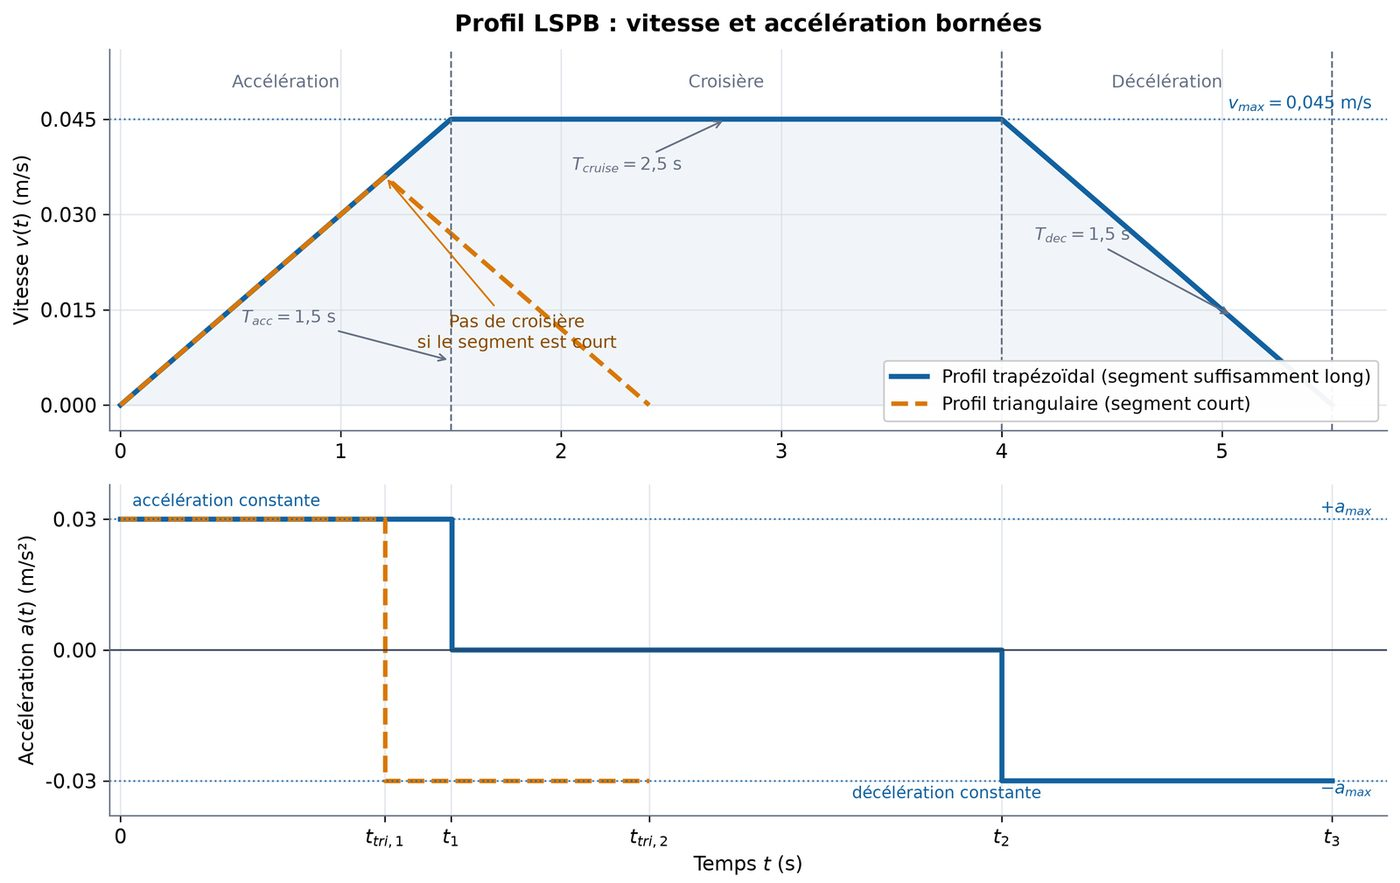
\includegraphics[width=0.95\textwidth]{lspb.jpg}
\caption{Profil de vitesse LSPB}
\label{fig:lspb}
\end{figure}

Le profil LSPB présente plusieurs avantages pour les trajectoires point-à-point \cite{lspb} :
\begin{itemize}
\item \textbf{Continuité de la vitesse} : la vitesse est nulle au départ et à l'arrivée, et continue pendant tout le mouvement.
\item \textbf{Accélération bornée} : l'accélération reste constante (ou nulle) sur chaque phase, ce qui évite les pics de couple.
\item \textbf{Implémentation simple} : le calcul des instants de transition est analytique, sans résolution numérique.
\item \textbf{Passage exact par les points} : contrairement aux B-splines, le robot passe exactement par chaque point de passage, ce qui est essentiel pour les applications de mesure.
\end{itemize}

En résumé, le \textbf{profil LSPB} constitue un bon compromis entre simplicité, continuité de la vitesse et respect des contraintes cinématiques. Il est particulièrement adapté aux trajectoires \textbf{point-à-point avec arrêt complet}, où les B-splines n'apportent pas de bénéfice significatif.

\section{Contraintes de planification}

La génération d'un chemin (section 2.2) et son lissage (section 2.3) ne suffisent pas à garantir qu'une trajectoire est réalisable. La planification doit en effet intégrer un ensemble de contraintes qui conditionnent le mouvement du robot. Ces contraintes se répartissent en quatre familles : mécaniques, cinématiques, visibilité et stabilité.

\subsection{Contraintes mécaniques}

Dans un robot parallèle à câbles, la contrainte mécanique fondamentale est l'\textbf{unilatéralité des câbles} : un câble ne peut transmettre qu'un effort de traction, jamais de poussée. Par conséquent, la tension dans chaque câble doit rester strictement positive à tout instant. En pratique, on impose une tension minimale $T_{\min}$ pour garantir que les câbles ne se détendent pas sous l'effet des perturbations, et une tension maximale $T_{\max}$ pour ne pas dépasser la capacité des moteurs ou la résistance des câbles.

Le respect simultané de ces bornes définit l'\textbf{espace de travail faisable en effort} (Wrench-Feasible Workspace, WFW), déjà introduit en section 1.5.4. Gouttefarde et al. \cite{gouttefarde2011} ont montré que le WFW peut être déterminé par une analyse par intervalles, qui garantit l'existence d'une distribution de tensions admissible pour une pose donnée. Une trajectoire n'est réalisable que si elle reste \textbf{intégralement incluse} dans le WFW. La planification doit donc vérifier, pour chaque point de la trajectoire, que le problème d'équilibre statique admet une solution en tensions respectant les bornes.



\subsection{Contraintes cinématiques}

Les contraintes cinématiques portent sur les \textbf{vitesses} et \textbf{accélérations} maximales que les actionneurs peuvent fournir, ainsi que sur le \textbf{jerk} (dérivée de l'accélération) lorsque la continuité de l'accélération est requise \cite{gasparetto2015}.

Pour un robot à câbles, ces contraintes se traduisent directement sur les vitesses de déroulement des câbles : $\dot{l}_i \leq \dot{l}_{\max}$ et $\ddot{l}_i \leq \ddot{l}_{\max}$. Ces limites sont imposées par la vitesse maximale des moteurs et par la capacité des enrouleurs à accélérer sans décrochage. La planification de trajectoire doit donc garantir que le profil de vitesse retenu (par exemple un profil LSPB, section 2.3.3) respecte ces bornes sur l'ensemble du chemin.

\subsection{Contraintes de visibilité}

Lorsque le robot embarque un capteur (caméra, lidar), la planification doit également respecter des contraintes de \textbf{visibilité} : le capteur doit être orienté vers la cible, à une distance et un angle compatible avec ses caractéristiques (champ de vision, résolution, profondeur de champ). Ces contraintes se traduisent par des exigences sur l'\textbf{orientation} de la plateforme et sur sa \textbf{position relative} par rapport aux points d'intérêt.

Dans le cas d'un robot à câbles, ces contraintes sont particulièrement délicates car l'orientation de la plateforme est souvent contrainte par la géométrie des câbles. Si l'orientation doit être pilotée, il faut vérifier que le WFW reste non vide pour la pose complète (position + orientation). Si l'orientation est fixe (comme dans le cas d'une plateforme en translation pure), les contraintes de visibilité se réduisent à des contraintes de position.

\subsection{Contraintes de stabilité}

Les robots à câbles sont sujets aux \textbf{vibrations}, en raison de la faible rigidité des câbles et de leur amortissement naturel très faible. Ces vibrations dégradent la précision du positionnement et augmentent le \textbf{temps d'établissement} : le temps nécessaire pour que la plateforme se stabilise à une position donnée après un mouvement.

Khayour \cite{khayour2022} souligne que la flexibilité des câbles réduit la bande passante des efforts qu'ils peuvent transmettre, ce qui limite la capacité à amortir les vibrations et à suivre des trajectoires dynamiques. Pour garantir la stabilité, la planification doit donc éviter les \textbf{à-coups} (jerk élevé) et prévoir des \textbf{temps d'arrêt} suffisants à chaque point de mesure ou d'opération. Ces temps d'arrêt, appelés temps de stabilisation, dépendent des caractéristiques vibratoires du système (fréquences propres, amortissement) et des exigences de précision.

\begin{figure}[H]
\centering
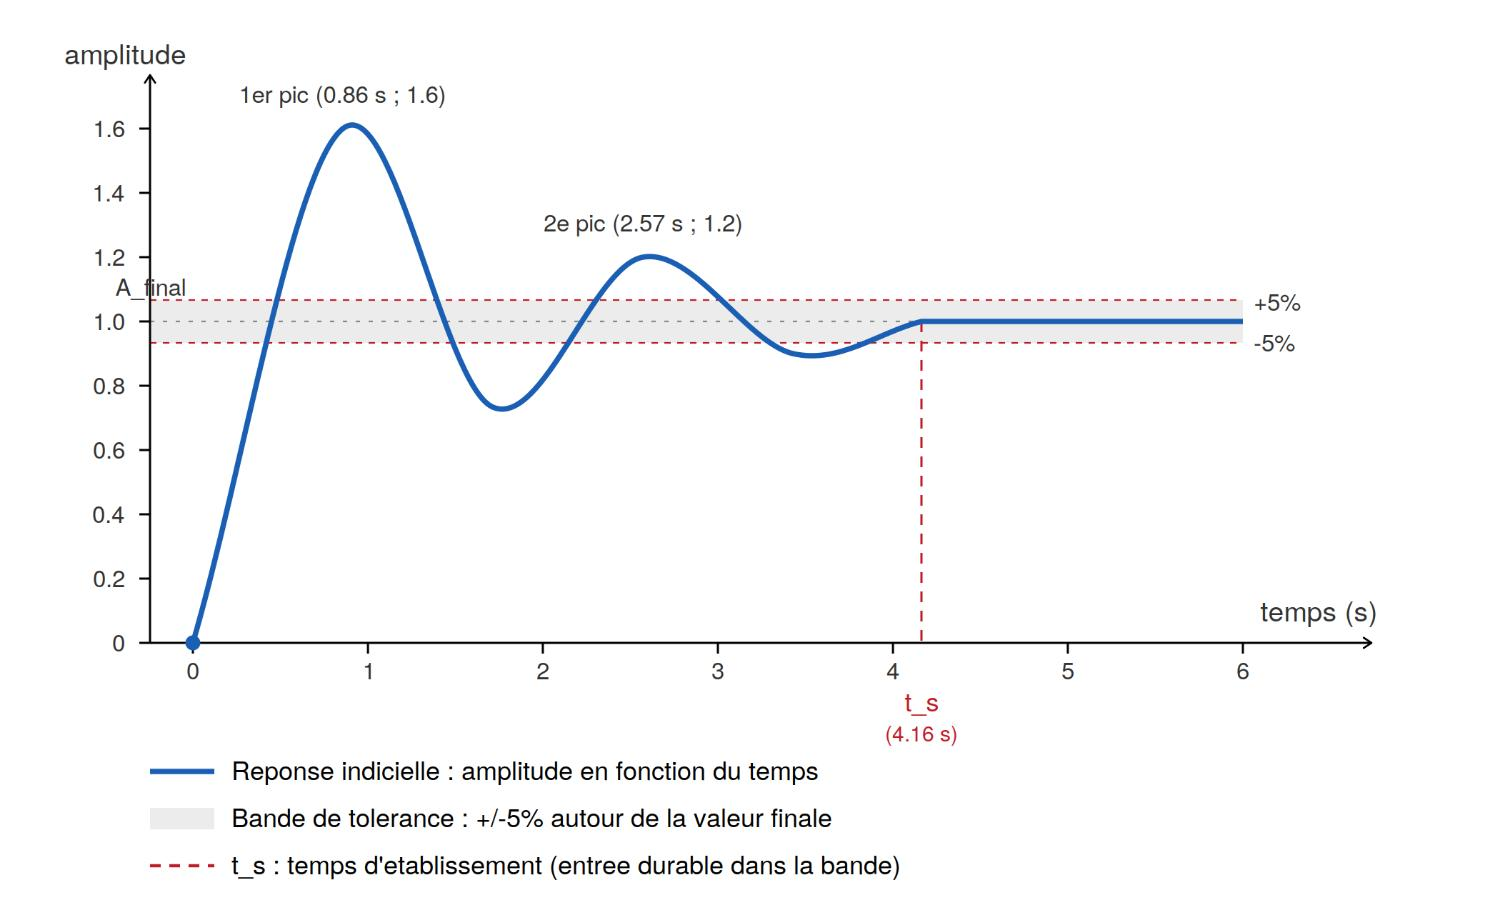
\includegraphics[width=0.72\textwidth]{systeme_vibratoire.png}
\caption{Réponse indicielle et temps d'établissement}
\label{fig:vibratoire}
\end{figure}

\section{Cadre d'optimisation}

La génération de chemin (section 2.2) et le lissage de trajectoire (section 2.3) produisent une trajectoire \textit{faisable}. Cependant, il existe généralement une \textbf{infinité de trajectoires faisables} pour une même tâche. Le cadre d'optimisation a pour objectif de sélectionner, parmi ces solutions, celle qui minimise (ou maximise) un ou plusieurs \textbf{critères de performance} tout en respectant les contraintes (section 2.4).

\begin{figure}[H]
\centering
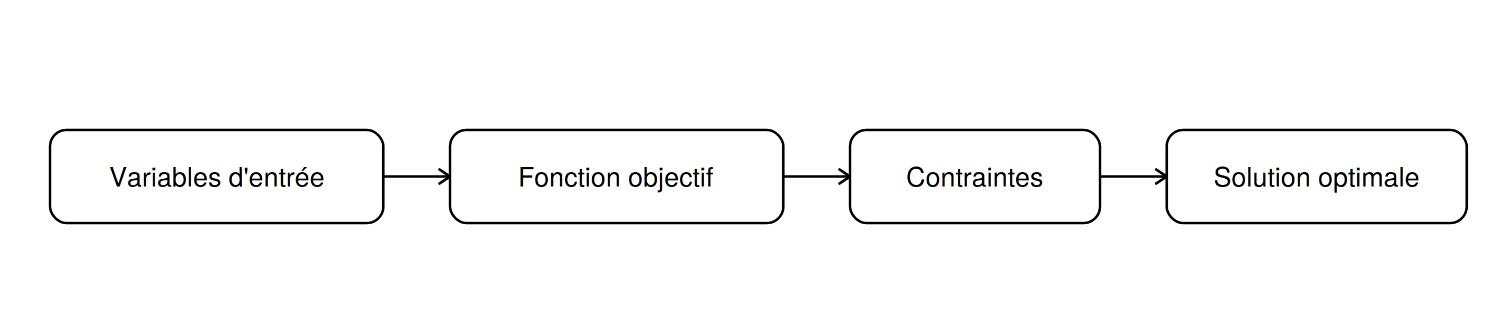
\includegraphics[width=0.80\textwidth]{probleme_optimisation.png}
\caption{Structure d'un problème d'optimisation}
\label{fig:optimisation}
\end{figure}

\subsection{Formulation du problème}

Un problème d'optimisation se formalise par trois éléments \cite{gasparetto2015} :
\begin{itemize}
\item \textbf{Variables de décision} : les paramètres (ordre de visite, instants de passage, paramètres du profil de vitesse, etc.).
\item \textbf{Fonction objectif} : la quantité à minimiser ou maximiser (temps, énergie, jerk, etc.).
\item \textbf{Contraintes} : les limitations à respecter (bornes de tension, limites de vitesse, contraintes de visibilité, etc.).
\end{itemize}

Mathématiquement :
\begin{equation}
\min_{\mathbf{x}} \quad f(\mathbf{x}) \quad \text{sous contraintes} \quad g_i(\mathbf{x}) \leq 0, \quad h_j(\mathbf{x}) = 0
\label{eq:optimisation}
\end{equation}
où
\begin{itemize}
\item $\mathbf{x}$ est le vecteur des variables de décision,
\item $f$ la fonction objectif,
\item $g_i$ les contraintes d'inégalité et
\item $h_j$ les contraintes d'égalité.
\end{itemize}

La difficulté du problème dépend de la nature de $f$ (linéaire, non linéaire, convexe) et des contraintes \cite{gasparetto2015}.

\subsection{Optimisation mono et multi-objectif}

Lorsqu'un seul critère est optimisé, on parle d'\textbf{optimisation mono-objectif} : la solution est unique (ou appartient à un ensemble d'indifférence). Les méthodes classiques (gradient, programmation linéaire) s'appliquent directement.

Lorsque plusieurs critères \textbf{conflictuels} doivent être optimisés simultanément (par exemple, minimiser le temps \textit{et} l'énergie), on parle d'\textbf{optimisation multi-objectif}. Il n'existe alors généralement pas de solution unique, mais un ensemble de solutions \textbf{non dominées} appelé \textbf{front de Pareto} \cite{gasparetto2015}. Une solution $A$ domine une solution $B$ si $A$ est meilleure ou égale sur tous les objectifs, et strictement meilleure sur au moins un. Le front de Pareto représente le meilleur compromis possible entre les objectifs.

\begin{figure}[H]
\centering
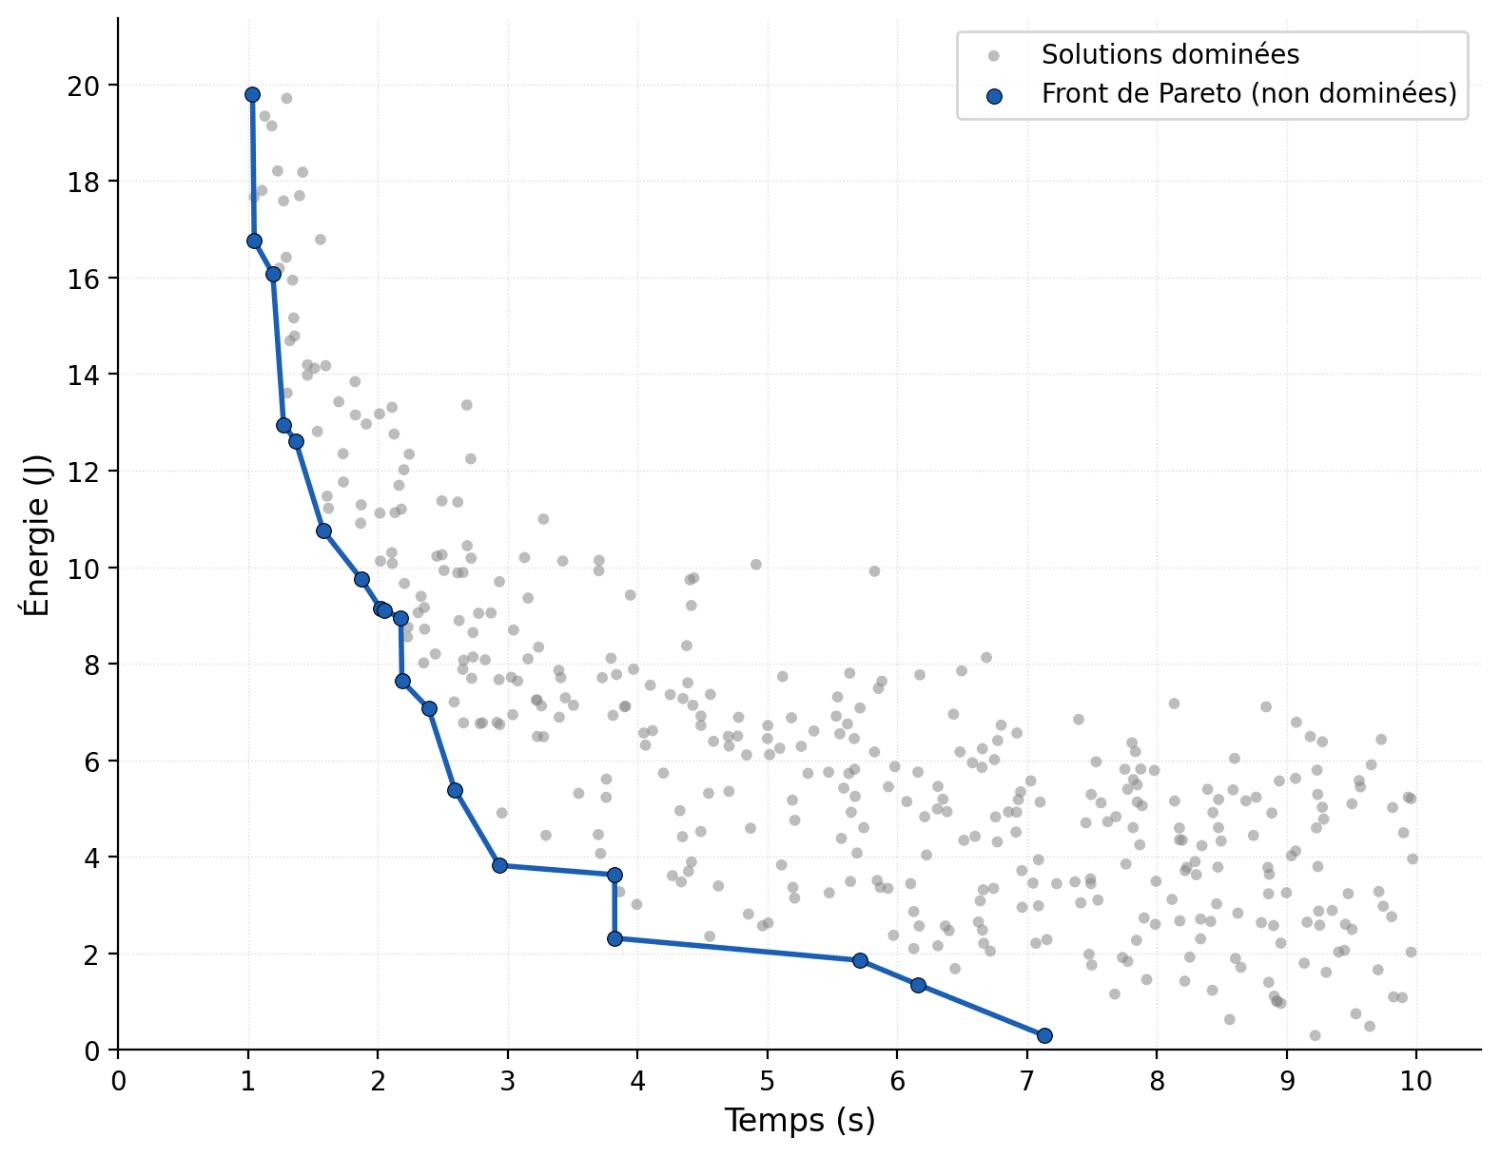
\includegraphics[width=0.72\textwidth]{front_pareto.png}
\caption{Front de Pareto (temps vs énergie)}
\label{fig:pareto}
\end{figure}

\subsection{Modèle énergétique}

Le \textbf{modèle énergétique} permet d'estimer la consommation d'énergie associée à une trajectoire. Pour un robot à câbles, l'énergie dépend principalement des tensions dans les câbles, des vitesses de déroulement, des accélérations et des pertes dans les moteurs \cite{gasparetto2015}, \cite{lspb}.

Un modèle simplifié consiste à intégrer la puissance mécanique sur la durée de la trajectoire :
\begin{equation}
E = \int_{0}^{T} \sum_{i=1}^{m} T_i(t) \, |\dot{l}_i(t)| \, dt
\label{eq:energie}
\end{equation}
où
\begin{itemize}
\item $T_i$ est la tension dans le câble $i$,
\item $\dot{l}_i$ sa vitesse de déroulement.
\end{itemize}

\subsection{Méthodes exactes}

Les \textbf{méthodes exactes} garantissent la solution optimale en un temps fini. Elles sont adaptées aux problèmes de petite taille ou de structure particulière \cite{gasparetto2015} : programmation linéaire (LP), programmation quadratique (QP), programmation dynamique, méthodes par branchement et bornes. Leur efficacité décroît rapidement lorsque le nombre de variables ou la non-linéarité augmentent. On recourt alors à des méthodes approchées.

\subsection{Métaheuristiques mono-objectif}

Les \textbf{métaheuristiques} sont des algorithmes d'optimisation de haut niveau, inspirés de phénomènes naturels, qui fournissent de bonnes solutions en un temps raisonnable sans garantir l'optimalité. Pour l'optimisation mono-objectif, les plus utilisées sont \cite{gasparetto2015} : recuit simulé, algorithmes génétiques (GA), optimisation par essaim particulaire (PSO), colonies de fourmis (ACO). Ces méthodes nécessitent un réglage de paramètres et peuvent converger vers des optimums locaux.

\subsection{Métaheuristiques multi-objectif}

Pour l'optimisation multi-objectif, les métaheuristiques doivent produire un \textbf{ensemble de solutions non dominées} (front de Pareto). Les algorithmes les plus utilisés sont \cite{gasparetto2015} : \textbf{NSGA-II}, \textbf{MOEA/D} et \textbf{MOPSO}. Parmi eux, NSGA-II \cite{deb2002} constitue un algorithme de référence pour les problèmes à deux ou trois objectifs. Sa robustesse, sa convergence rapide et sa capacité à maintenir un front bien réparti en font une méthode largement étudiée dans la littérature.

\subsubsection{Principe général du NSGA-II}

NSGA-II est un \textbf{algorithme génétique} : il fait évoluer une \textbf{population} d'individus (solutions candidates) au fil de \textbf{générations} successives, en appliquant les principes de sélection, croisement et mutation. Ce qui le distingue d'un algorithme génétique classique, c'est sa capacité à gérer \textbf{plusieurs objectifs simultanément} en classant les individus selon leur \textbf{dominance} et en préservant la \textbf{diversité} du front de Pareto \cite{deb2002}.

Un individu (ou chromosome) code une solution candidate. Selon la nature du problème, le codage peut être \textbf{réel} (paramètres continus), \textbf{par permutation} (ordre de visite) ou \textbf{binaire}.

\subsubsection{Étapes de l'algorithme}

\textbf{Étape 1 : Initialisation.}

Une population initiale de $N$ individus est générée aléatoirement. Chaque individu est évalué selon les $M$ objectifs, ce qui donne un vecteur de coûts $(f_1, f_2, \ldots, f_M)$.

\begin{figure}[!htbp]
\centering
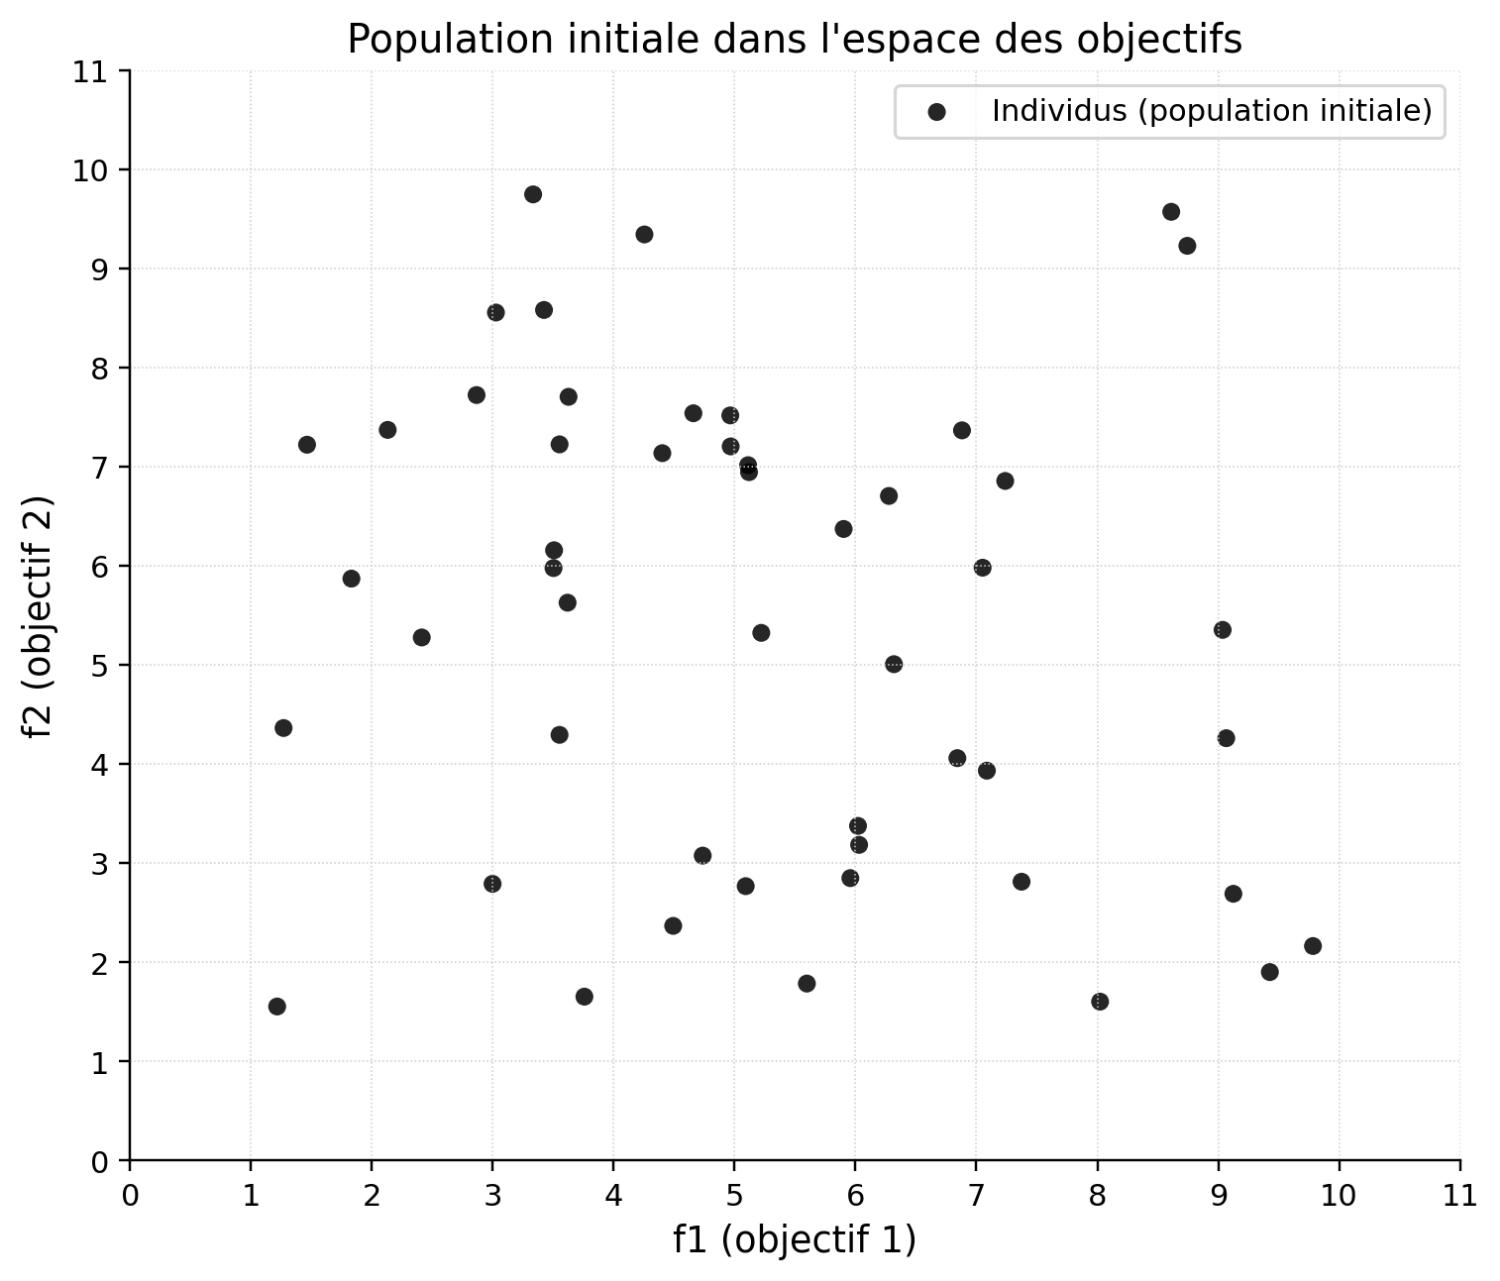
\includegraphics[width=0.65\textwidth]{population_initiale.png}
\caption{Population initiale (espace des objectifs)}
\label{fig:pop_init}
\end{figure}

\textbf{Étape 2 : Tri non-dominé.}

Les individus sont classés en \textbf{fronts successifs} : front 1 (non dominés), front 2 (non dominés après retrait du front 1), etc. Chaque individu reçoit un \textbf{rang} correspondant à son front. Plus le rang est bas, la solution est meilleure.

\begin{figure}[H]
\centering
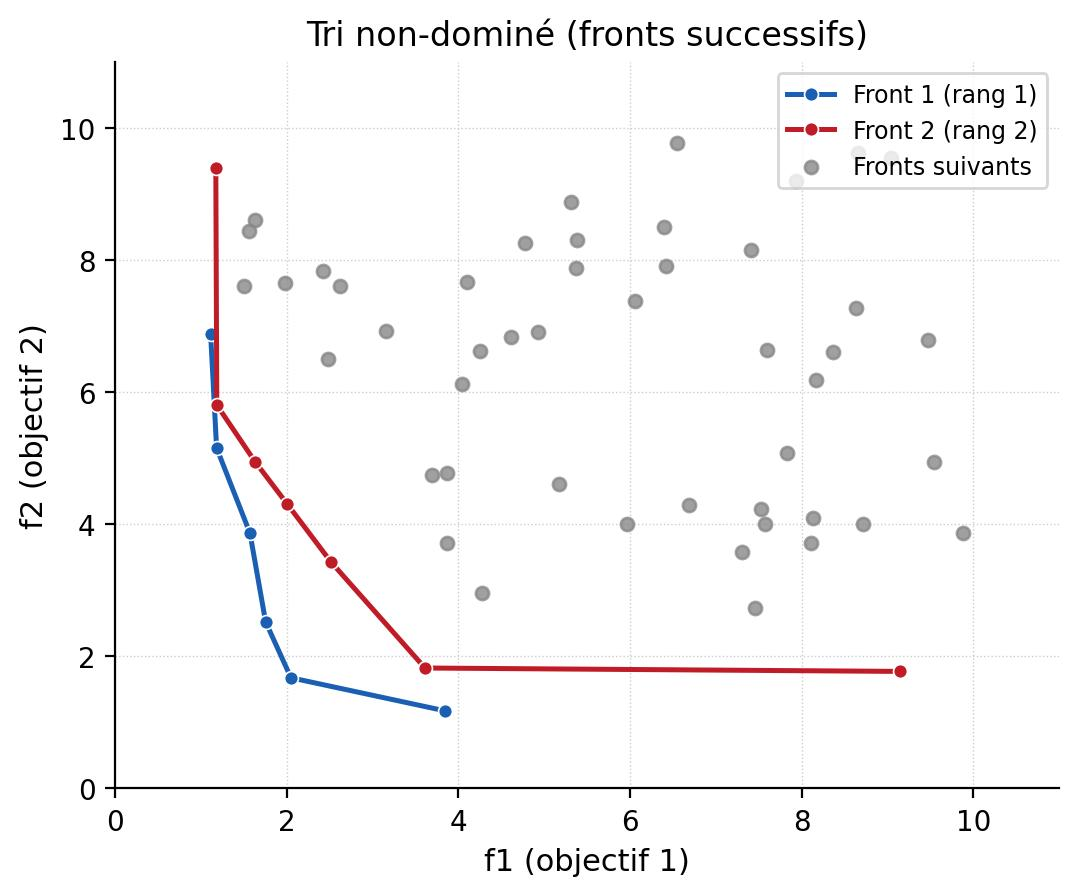
\includegraphics[width=0.70\textwidth]{tri_non_domine.png}
\caption{Tri non-dominé en fronts successifs}
\label{fig:tri}
\end{figure}

\textbf{Étape 3 : Distance de peuplement.}

Pour préserver la \textbf{diversité} du front, NSGA-II calcule pour chaque individu une \textbf{distance de peuplement} : la distance moyenne qui le sépare de ses voisins dans l'espace des objectifs. Un individu isolé est préféré à un individu entassé.

\begin{figure}[H]
\centering
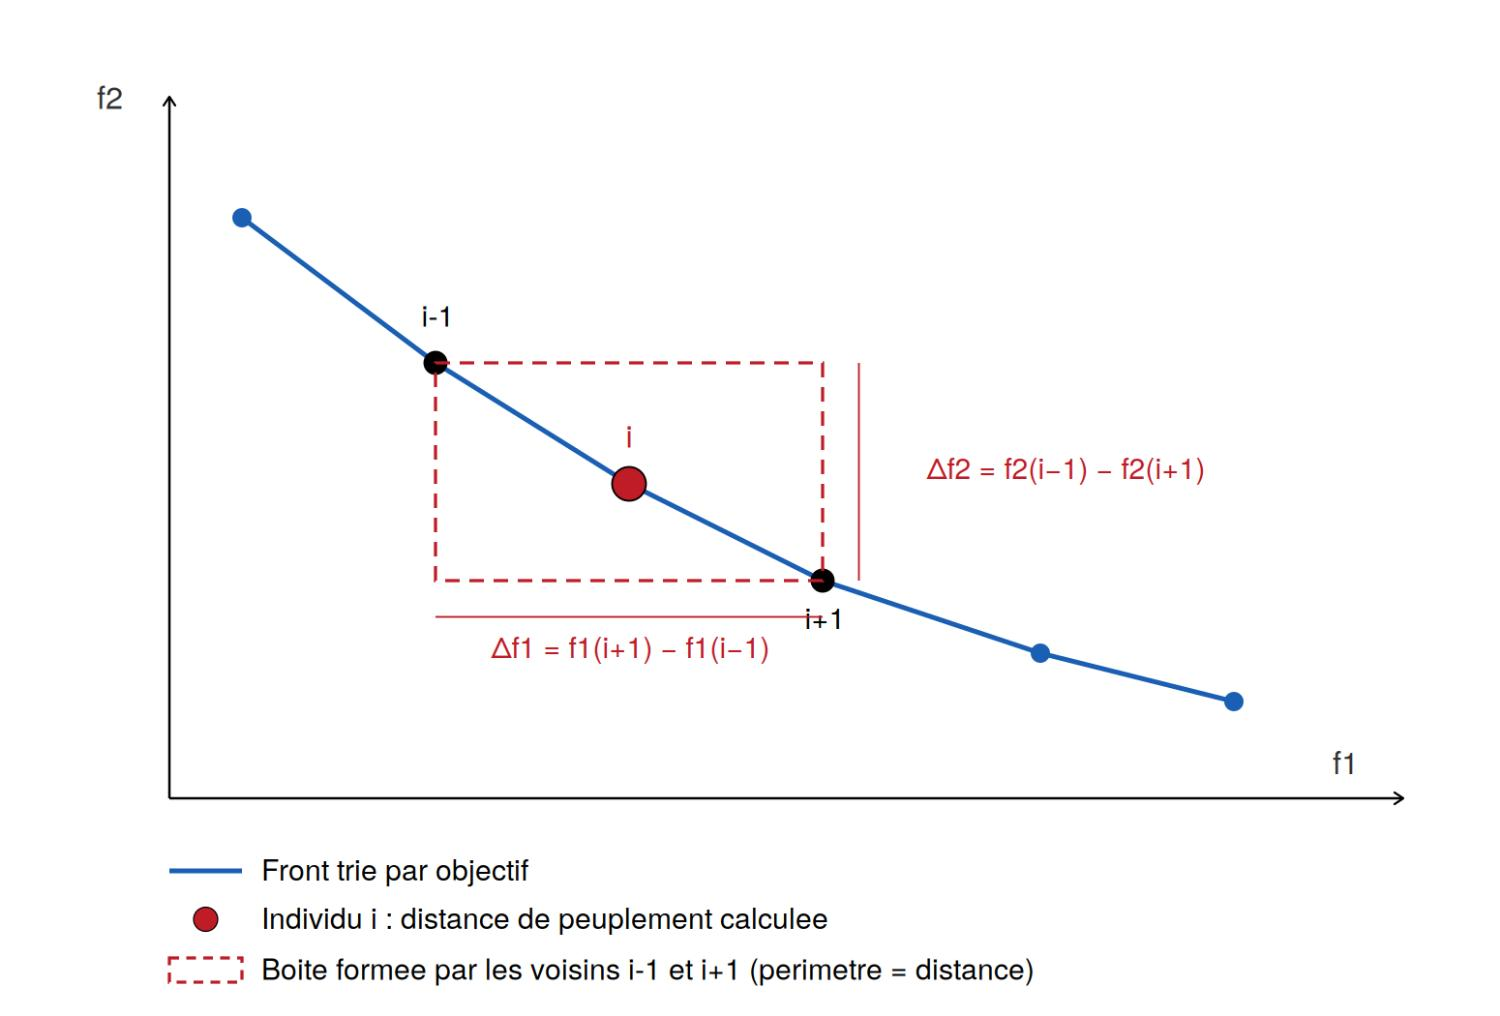
\includegraphics[width=0.72\textwidth]{distance_peuplement.png}
\caption{Distance de peuplement}
\label{fig:distance}
\end{figure}

\textbf{Étape 4 : Sélection des parents.}

Les individus sont sélectionnés par \textbf{tournoi binaire}. Le critère est : d'abord le rang (le plus bas est préféré), puis la distance de peuplement (la plus élevée est préférée). Ce mécanisme favorise à la fois la \textbf{convergence} et la \textbf{diversité}.

\textbf{Étape 5 : Croisement et mutation.}

Les parents sont croisés deux à deux pour produire des enfants. L'opérateur dépend du codage : croisement barycentrique (SBX) pour le réel, croisement d'ordre (OX) ou partiellement apparié (PMX) pour les permutations. Les enfants subissent ensuite une \textbf{mutation} aléatoire (taux typique : 5 à 10 \%).

\textbf{Étape 6 : Combinaison parents et enfants.}

Les deux populations ($N$ parents + $N$ enfants) sont \textbf{fusionnées} pour former une population temporaire de $2N$ individus. Cette étape garantit l'\textbf{élitisme}.

\textbf{Étape 7 : Tri non-dominé de la population combinée.}

La population combinée est triée selon le même principe. La nouvelle population de $N$ individus est remplie en prenant les fronts dans l'ordre. Si un front dépasse la place restante, les individus \textbf{les mieux répartis} sont sélectionnés selon leur distance de peuplement.

\textbf{Étape 8 : Répétition.}

Les étapes 2 à 7 sont répétées sur un nombre fixé de générations ou jusqu'à un critère d'arrêt. La population finale contient le \textbf{front de Pareto} approximé.

\begin{figure}[H]
\centering
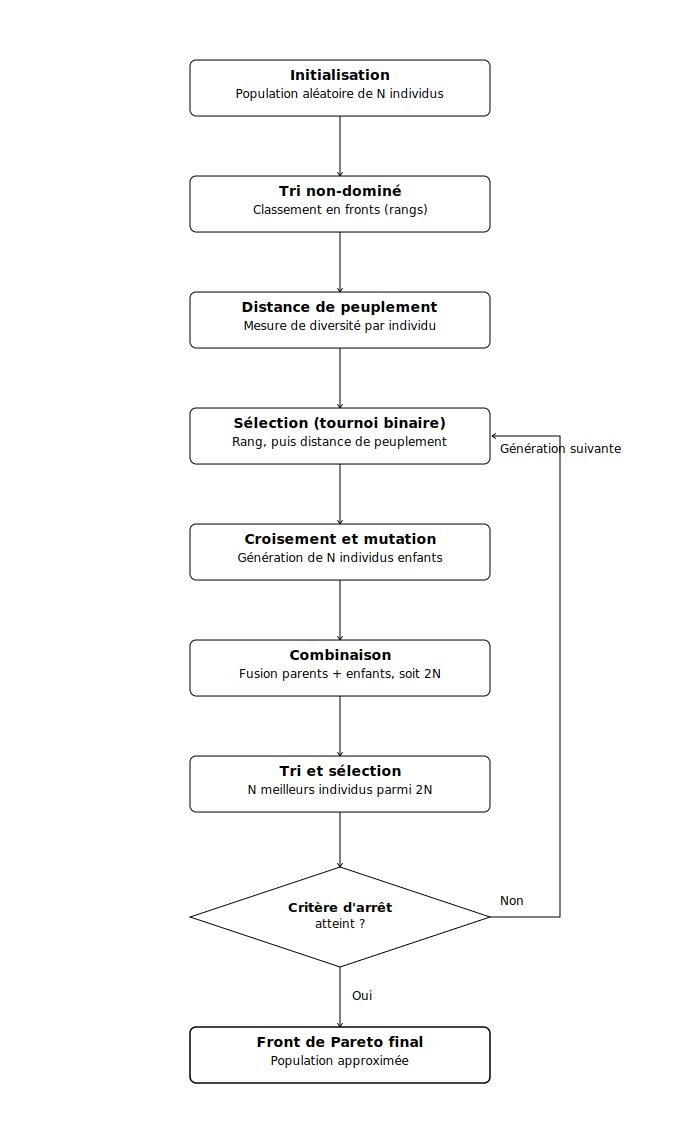
\includegraphics[width=0.58\textwidth]{organigramme_nsga2.png}
\caption{Organigramme de NSGA-II}
\label{fig:nsga2}
\end{figure}



\subsubsection{Avantages et limites}

\begin{itemize}
\item \textbf{Avantages} : convergence rapide, bonne répartition des solutions, élitisme, complexité maîtrisée $O(M N^2)$.
\item \textbf{Limites} : efficacité décroissante au-delà de 3 objectifs, sensibilité au réglage des paramètres, pas de garantie d'optimalité globale.
\end{itemize}

\section{Robustesse d'une trajectoire}

La planification de trajectoire présentée dans les sections précédentes repose sur un \textbf{modèle nominal} du robot et de son environnement. En pratique, le modèle n'est qu'une approximation : les paramètres physiques sont incertains, les mesures sont bruitées, et des perturbations externes peuvent survenir en cours d'exécution. La \textbf{robustesse} désigne la capacité d'une trajectoire à rester performante malgré ces incertitudes.

\subsection{Sources d'incertitude}

Les incertitudes qui affectent la planification et l'exécution d'une trajectoire robotique peuvent être classées en trois familles \cite{puphal2026} :

\begin{itemize}
\item \textbf{Incertitudes de modèle.}
Le modèle géométrique et dynamique du robot est une approximation de la réalité. Les paramètres physiques (masses, inerties, longueurs, raideurs) sont connus avec une précision limitée, et certains phénomènes (frottements, élasticité, jeu mécanique) sont négligés ou simplifiés. Dans le cas des robots à câbles, l'élasticité des câbles et leur affaissement sous poids propre introduisent des écarts entre le modèle rigide et le comportement réel \cite{khayour2022}.

\item \textbf{Incertitudes de mesure.}
Les capteurs (codeurs, accéléromètres, capteurs de force) fournissent des mesures entachées de bruit, avec une résolution et une bande passante finies. L'estimation de la pose réelle de la plateforme à partir de ces mesures est donc imparfaite, ce qui peut conduire à des erreurs de suivi de trajectoire.

\item \textbf{Perturbations externes.}
L'environnement d'exécution peut être source de perturbations non modélisées : vent, vibrations du bâti, chocs, variations de température. Ces perturbations sont critiques pour les robots à câbles, dont la faible rigidité les rend sensibles aux efforts extérieurs \cite{khayour2022}. Une rafale de vent peut faire chuter la tension d'un câble sous son seuil minimal et compromettre la stabilité du système.
\end{itemize}

\begin{figure}[H]
\centering
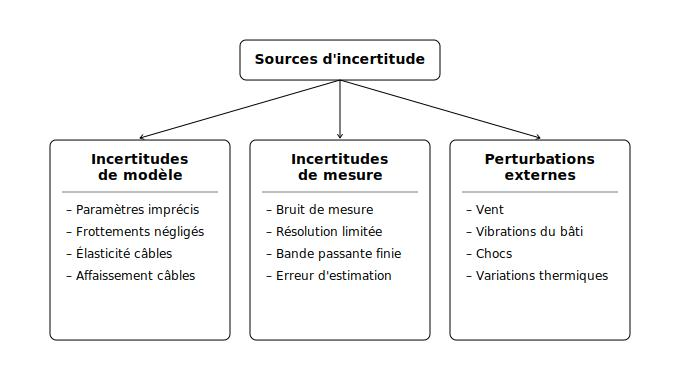
\includegraphics[width=0.85\textwidth]{incertitude.png}
\caption{Sources d'incertitude}
\label{fig:incertitudes}
\end{figure}

\section*{Conclusion}

Ce chapitre a présenté les fondements théoriques de la planification et de l'optimisation de trajectoires, en distinguant path planning et trajectory planning, et en détaillant les méthodes de génération de chemin, de lissage, les contraintes mécaniques, cinématiques, de visibilité et de stabilité, ainsi que le cadre d'optimisation mono- et multi-objectif et les stratégies de robustesse. Les principales approches ont été décrites, comme la couverture complète, la tournée de points, le profil LSPB, le front de Pareto et l'algorithme NSGA-II. Ce cadre général reste indépendant de tout système physique particulier : il ne permet pas encore de choisir entre les différentes méthodes, ni d'anticiper les contraintes propres à un robot à câbles telles que la faible rigidité ou les limites de tension. C'est cette confrontation à un cas concret qui doit permettre de sélectionner, parmi les outils présentés, ceux les mieux adaptés à ces contraintes spécifiques. Le chapitre suivant est ainsi consacré à l'étude du robot Tandem, qui applique ces concepts à un système réel et en tire les choix méthodologiques correspondants.




\clearpage
% ============================================================
% CHAPITRE III
% ============================================================

\chapter{ÉTUDE DU ROBOT TANDEM}

Ce chapitre applique au robot Tandem les concepts théoriques des chapitres précédents. Il présente l'architecture du robot et ses contraintes mécaniques, puis la chaîne de traitement en quatre macro-blocs. Il détaille ensuite la campagne de tests qui dimensionne l'algorithme NSGA-II, avant d'exposer les résultats sur deux tailles de grille et l'effet de la couverture de la zone de travail sur le temps et l'énergie.

\section{Architecture et modélisation du robot Tandem}

\subsection{Présentation du robot et de la charge utile}

Le robot Tandem est un robot parallèle à câbles (CDPR) à 8 câbles, pleinement contraint en statique : il dispose de 6 degrés de liberté (3 forces et 3 moments). La trajectoire est planifiée en translation pure et l'orientation de la plateforme reste fixe ($\mathbf{R}=\mathbf{I}$). Selon la classification du chapitre~I, le robot est redondant :
\begin{itemize}
\item en 6~DDL : $m = 8 > n+1 = 7$ ;
\item en 3~DDL de translation : $m = 8 > n+1 = 4$.
\end{itemize}
Cette redondance de deux câbles offre plusieurs distributions de tension pour une même pose et aide à maintenir des tensions positives. Elle ne garantit pas à elle seule l'existence d'une solution mécanique : la faisabilité doit être vérifiée à chaque position, sous contraintes.

\begin{figure}[H]
\centering
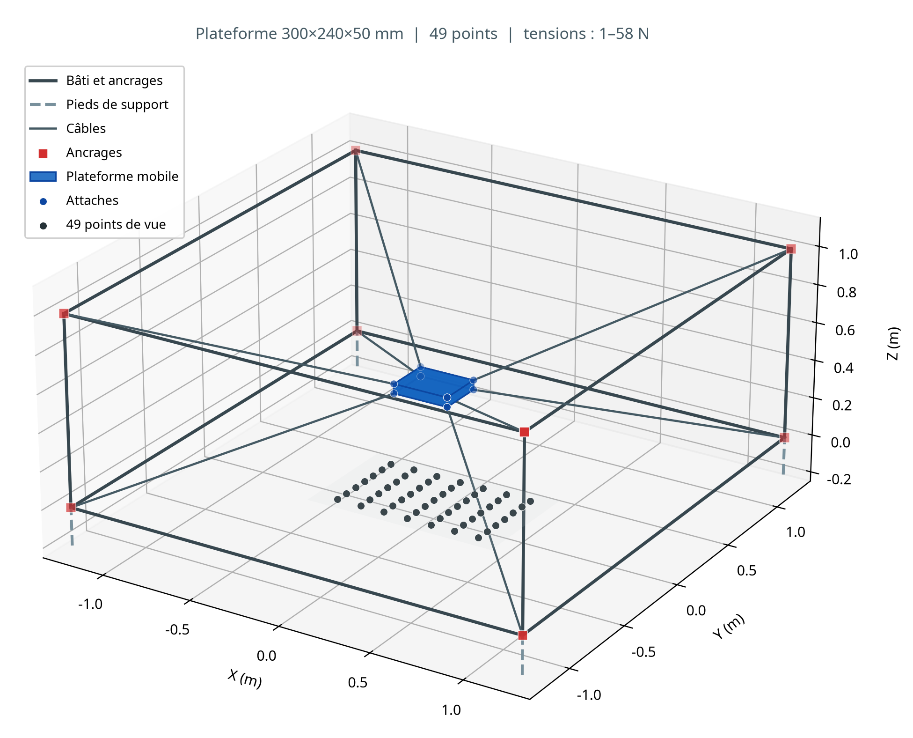
\includegraphics[width=0.92\textwidth,height=0.55\textheight,keepaspectratio]{robot_tandem_fig.png}
\caption{Robot Tandem}
\label{fig:robot_tandem}
\end{figure}

La plateforme est un cadre rigide en aluminium 6061-T6 qui porte les 8 points d'attache des câbles et la charge utile (module caméra Raspberry~Pi et électronique de contrôle). La caméra est orientée en vue nadir (verticale) et fixée sous la plateforme, conformément au protocole défini avec le SP3.

\begin{table}[H]
\centering
\caption{Caractéristiques de la plateforme mobile}
\label{tab:plateforme}
\begin{tabular}{|p{4.5cm}|p{5.5cm}|p{3.5cm}|}
\hline
\textbf{Paramètre} & \textbf{Valeur} & \textbf{Origine} \\
\hline
Matériau & Aluminium 6061-T6 & Choix de conception \\
\hline
Dimensions & $300 \times 240$~mm (ratio d'aspect 1,25) & Choix de conception \\
\hline
Masse à vide & $\approx 242$~g & Mesure \\
\hline
Charge utile & $\approx 114$~g & Somme des composants \\
\hline
Marge câblage et fixations & 8~\% & Hypothèse \\
\hline
Masse opérationnelle & 384~g & Calcul avec marge \\
\hline
Points d'attache & 8 & Choix de conception \\
\hline
\end{tabular}
\end{table}

\begin{table}[H]
\centering
\caption{Composition de la charge utile}
\label{tab:charge}
\begin{tabular}{|p{5.5cm}|p{2.2cm}|p{5.5cm}|}
\hline
\textbf{Composant} & \textbf{Masse} & \textbf{Rôle} \\
\hline
Raspberry Pi Zero 2 W & 11~g & Unité de calcul \\
\hline
Pi Camera Module 3 & 4,3~g & Capteur d'image RGB \\
\hline
Câble nappe CSI & 5~g & Liaison caméra et Pi \\
\hline
Cellule 18650 avec porte-pile & 47~g & Alimentation \\
\hline
Convertisseur (boost) & 12~g & Conversion 3,7~V vers 5~V \\
\hline
Capteur HC-SR04 & 5~g & Distance aux plants \\
\hline
Accéléromètre 3 axes & 10~g & Vérification de la stabilité \\
\hline
Boîtier de protection & 20~g & Protection \\
\hline
Total & $\approx 114$~g & \\
\hline
\end{tabular}
\end{table}

La masse à vide (242~g) et la charge utile ($\approx 114$~g) donnent environ 356~g. Avec la marge de 8~\% pour le câblage et les fixations, on obtient la masse opérationnelle de 384~g. C'est elle, et non la masse à vide, qui est utilisée dans tous les calculs mécaniques.

\subsection{Modèle géométrique inverse et contraintes}

Le modèle géométrique inverse (MGI) calcule la longueur de chaque câble à partir de la position $\mathbf{p}$ de la plateforme. L'orientation étant fixe, le calcul se réduit à une distance euclidienne entre l'ancrage $\mathbf{A}_i$ et l'attache $\mathbf{B}_i(\mathbf{p}) = \mathbf{p} + \mathbf{b}_i$ :
\begin{equation}
l_i = \sqrt{(A_{ix}-B_{ix}(\mathbf{p}))^2 + (A_{iy}-B_{iy}(\mathbf{p}))^2 + (A_{iz}-B_{iz}(\mathbf{p}))^2}
\label{eq:mgi}
\end{equation}
Les coordonnées des ancrages et des attaches sont définies dans la configuration de référence. Les câbles 1 à 4 sont les câbles hauts (ancrages à $z=1{,}00$~m) et les câbles 5 à 8 les câbles bas (ancrages à $z=0$).

La plateforme est évaluée à la hauteur de référence $z = 0{,}45$~m dans le repère fixe. Cette hauteur découle de la mission : distance opérationnelle capteur--plants de 0,30~m, hauteur de plants de 0,35~m et décalage sol/repère de 0,20~m.

\paragraph{Application numérique.}
Pour $\mathbf{p}=(0,\,0,\,0{,}45)$~m et $\mathbf{b}_i = (\pm 0{,}150;\,\pm 0{,}120;\,\pm 0{,}025)$~m :
\begin{equation}
\mathbf{B}_1 = (-0{,}150;\,0{,}120;\,0{,}475),\quad
l_1 = \sqrt{2{,}7625} \approx 1{,}662~\text{m}
\label{eq:l1}
\end{equation}
\begin{equation}
\mathbf{B}_5 = (-0{,}150;\,0{,}120;\,0{,}425),\quad
l_5 \approx 1{,}633~\text{m}
\label{eq:l5}
\end{equation}
Les six autres câbles se déduisent par symétrie.

\begin{table}[H]
\centering
\caption{Longueurs de câbles à la position centrale}
\label{tab:longueurs}
\begin{tabular}{|c|c|c|c|}
\hline
\textbf{Câble} & \textbf{Longueur (m)} & \textbf{Câble} & \textbf{Longueur (m)} \\
\hline
1 & 1,662 & 5 & 1,633 \\
\hline
2 & 1,662 & 6 & 1,633 \\
\hline
3 & 1,662 & 7 & 1,633 \\
\hline
4 & 1,662 & 8 & 1,633 \\
\hline
\end{tabular}
\end{table}

Les câbles du haut sont plus longs d'environ 2,9~cm que ceux du bas. Le poids de la plateforme vaut :
\begin{equation}
\mathbf{F}_{ext} = (0,\,0,\,-mg,\,0,\,0,\,0),\qquad mg = 0{,}384 \times 9{,}81 \approx 3{,}77~\text{N}
\label{eq:poids}
\end{equation}

\subsection{Espace de travail faisable (WFW) et singularité}

L'espace de travail faisable en tension (WFW) est déterminé par un test de faisabilité en effort, résolu par programmation linéaire (solveur HiGHS) :
\begin{equation}
\min_{\mathbf{T}}\ \mathbf{0}^{\top}\mathbf{T}
\quad\text{s.c.}\quad
\mathbf{W}(\mathbf{p})\,\mathbf{T} = -\mathbf{F}_{ext},
\quad T_{\min}\le T_i \le T_{\max}
\label{eq:wfw_lp}
\end{equation}
La matrice de structure $\mathbf{W}(\mathbf{p})\in\mathbb{R}^{6\times 8}$ s'écrit :
\begin{equation}
\mathbf{W} = \bigl[\ \mathbf{U}_i \ ;\ \mathbf{B}_i\times\mathbf{U}_i\ \bigr]_{i=1..8},
\quad
\mathbf{U}_i=\frac{\mathbf{A}_i-\mathbf{B}_i}{|\mathbf{A}_i-\mathbf{B}_i|}
\label{eq:W}
\end{equation}

\paragraph{Application numérique : câble 1 au centre.}
\begin{equation}
\mathbf{U}_1 \approx (-0{,}662;\,0{,}680;\,0{,}316),\quad
\mathbf{m}_1 \approx (-0{,}285;\,-0{,}267;\,-0{,}023)
\label{eq:u1}
\end{equation}
Avec $T_{\mathrm{haut}}=58$~N et $T_{\mathrm{bas}}=1$~N :
\begin{equation}
\sum F_z \approx 73{,}3 - 1{,}04 = 72{,}3~\text{N}
\label{eq:fz}
\end{equation}
Cette valeur dépasse largement le poids de 3,77~N : il existe une infinité de distributions admissibles.

Avant de résoudre le LP, le test contrôle le rang de $\mathbf{W}$. Si $\operatorname{rang}(\mathbf{W})<6$, le point est infaisable. Pour une plateforme carrée, le moment de lacet est identiquement nul et le rang tombe à~5. Pour la plateforme rectangulaire $300\times240$~mm (ratio 1,25), le rang reste égal à~6. La condition pratique retenue est un ratio d'aspect $\ge 1{,}20$.

\subsection{Configuration de référence}

\begin{table}[H]
\centering
\caption{Paramètres mécaniques et contraintes de la configuration de référence}
\label{tab:ref}
\footnotesize
\begin{tabular}{|p{4.0cm}|p{2.0cm}|p{1.8cm}|p{5.5cm}|}
\hline
\textbf{Paramètre} & \textbf{Valeur} & \textbf{Unité} & \textbf{Origine ou justification} \\
\hline
Plateforme & $300 \times 240$ & mm & Ratio d'aspect $1{,}25 \ge 1{,}20$ \\
\hline
Masse opérationnelle & 0,384 & kg & Mesure et marge de 8~\% \\
\hline
Tension minimale $T_{\min}$ & 1,0 & N & 100~\% de couverture \\
\hline
Tension maximale $T_{\max}$ & 58,0 & N & Borne de dimensionnement \\
\hline
Bornes zone sécurisée, X & $\pm 0{,}40$ & m & Mode zero-loss \\
\hline
Bornes zone sécurisée, Y & $\pm 0{,}24$ & m & Mode zero-loss \\
\hline
Limites verticales Z & $[0\,;\,0{,}80]$ & m & Configuration historique \\
\hline
Hauteur de référence & 0,45 & m & Dans le repère fixe \\
\hline
Distance capteur--plants & 0,30 & m & Protocole SP3 \\
\hline
Vitesse maximale $v_{\max}$ & 0,045 & m/s & Hypothèse de conception \\
\hline
Accélération maximale $a_{\max}$ & 0,03 & m/s$^2$ & Hypothèse de conception \\
\hline
Temps de stabilisation & 2,0 & s/point & Évite le flou de mouvement \\
\hline
\end{tabular}
\end{table}

La borne $T_{\max}=58$~N suppose une réduction d'environ 5:1 sur un moteur NEMA~17. La fenêtre de service couvre des plants jusqu'à 0,50~m (haricot nain). Le mode zero-loss désigne une zone resserrée garantissant 100~\% de points faisables.

\section{Chaîne de traitement en quatre macro-blocs}
\label{sec:macro}

Le pipeline comprend douze sous-blocs regroupés en quatre macro-blocs. Cette modularité apporte testabilité, traçabilité et parallélisation.

\begin{figure}[H]
\centering
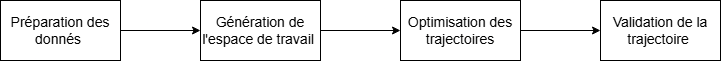
\includegraphics[width=0.95\textwidth,height=0.42\textheight,keepaspectratio]{macrobloc.png}
\caption{Chaîne de traitement en quatre macro-blocs}
\label{fig:macro}
\end{figure}

\begin{table}[H]
\centering
\caption{Correspondance des quatre macro-blocs}
\label{tab:macro}
\footnotesize
\begin{tabular}{|p{4.5cm}|p{4.0cm}|p{5.0cm}|}
\hline
\textbf{Macro-bloc} & \textbf{Rôle} & \textbf{Entrées et sorties} \\
\hline
1. Préparation des données & Paramètres, $\mathbf{W}$, MGI & Paramètres $\to$ configuration, $\mathbf{W}$ \\
\hline
2. Génération de l'espace de travail & Faisabilité, points retenus & Configuration $\to$ points filtrés \\
\hline
3. Optimisation des trajectoires & Matrice de coûts, ordre optimal & Points filtrés $\to$ solutions \\
\hline
4. Validation de la trajectoire & Profilage, vérification & Trajectoires $\to$ profils, rapport \\
\hline
\end{tabular}
\end{table}

\subsection{Préparation des données}

Le sous-bloc~0 centralise les paramètres dans une structure immuable après validation. Huit règles de validation lèvent une erreur explicite en cas de conflit.

\begin{figure}[H]
\centering
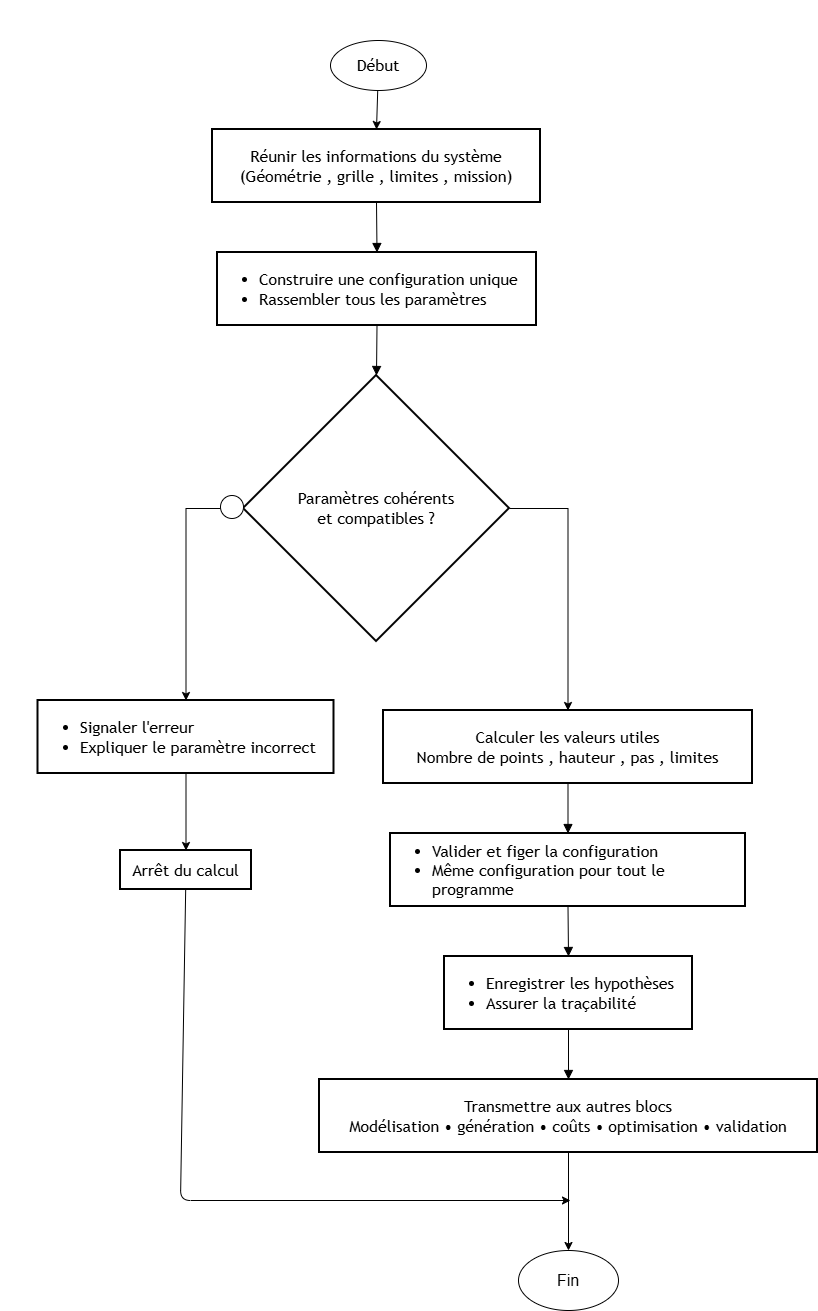
\includegraphics[width=0.95\textwidth,height=0.62\textheight,keepaspectratio]{bloc0.png}
\caption{Organigramme de la configuration}
\label{fig:bloc0}
\end{figure}

Le sous-bloc~1 construit $\mathbf{W}$ et le sous-bloc~2 assure la cinématique (MGI fermé, MGD par moindres carrés non linéaires).

\subsection{Génération de l'espace de travail}

Le sous-bloc~4 génère une grille centrée ; le sous-bloc~5 filtre par le test WFW précédé du test de rang. Le centre joue le rôle de verrou.

\clearpage
\begin{figure}[H]
\centering
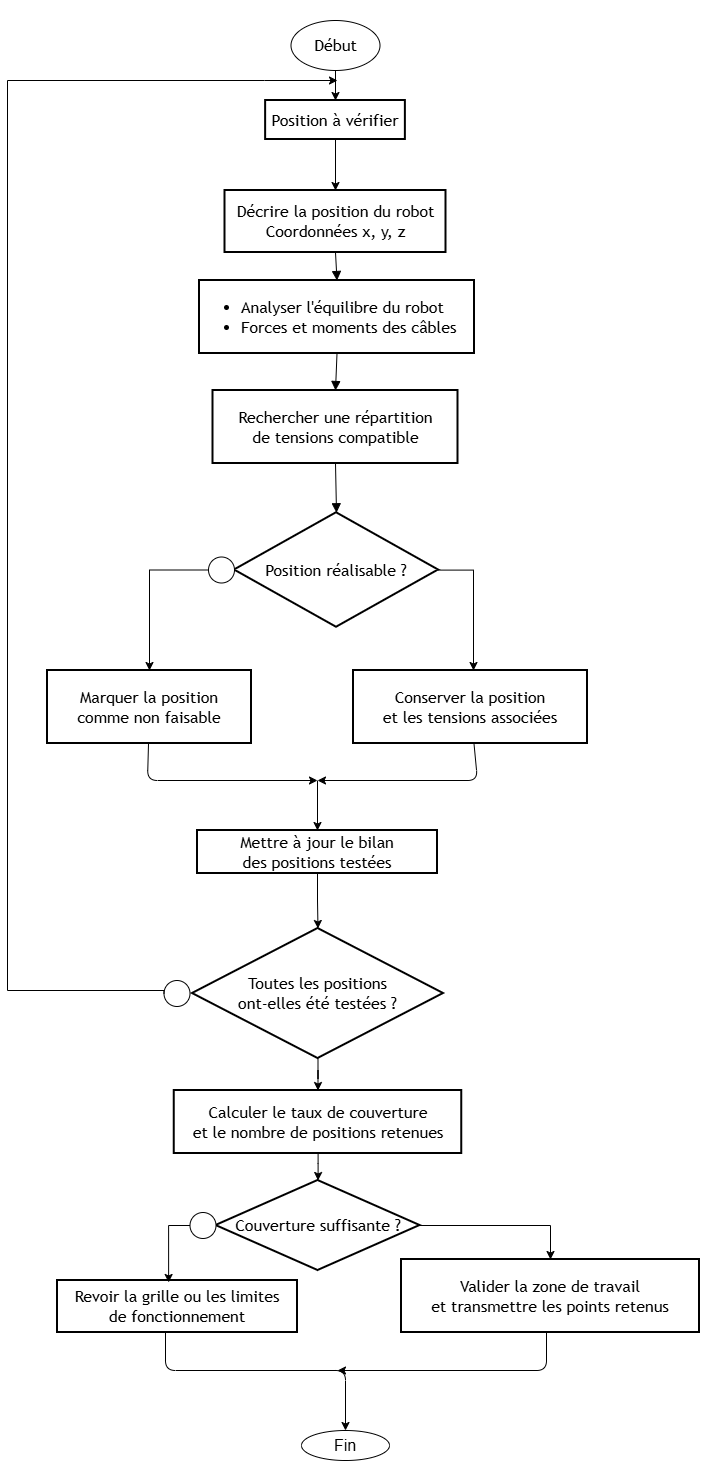
\includegraphics[width=\textwidth,height=0.90\textheight,keepaspectratio]{bloc3.png}
\caption{Organigramme du test WFW}
\label{fig:bloc3}
\end{figure}
\clearpage

\subsection{Optimisation des trajectoires}
\label{sec:macro3}

\begin{figure}[H]
\centering
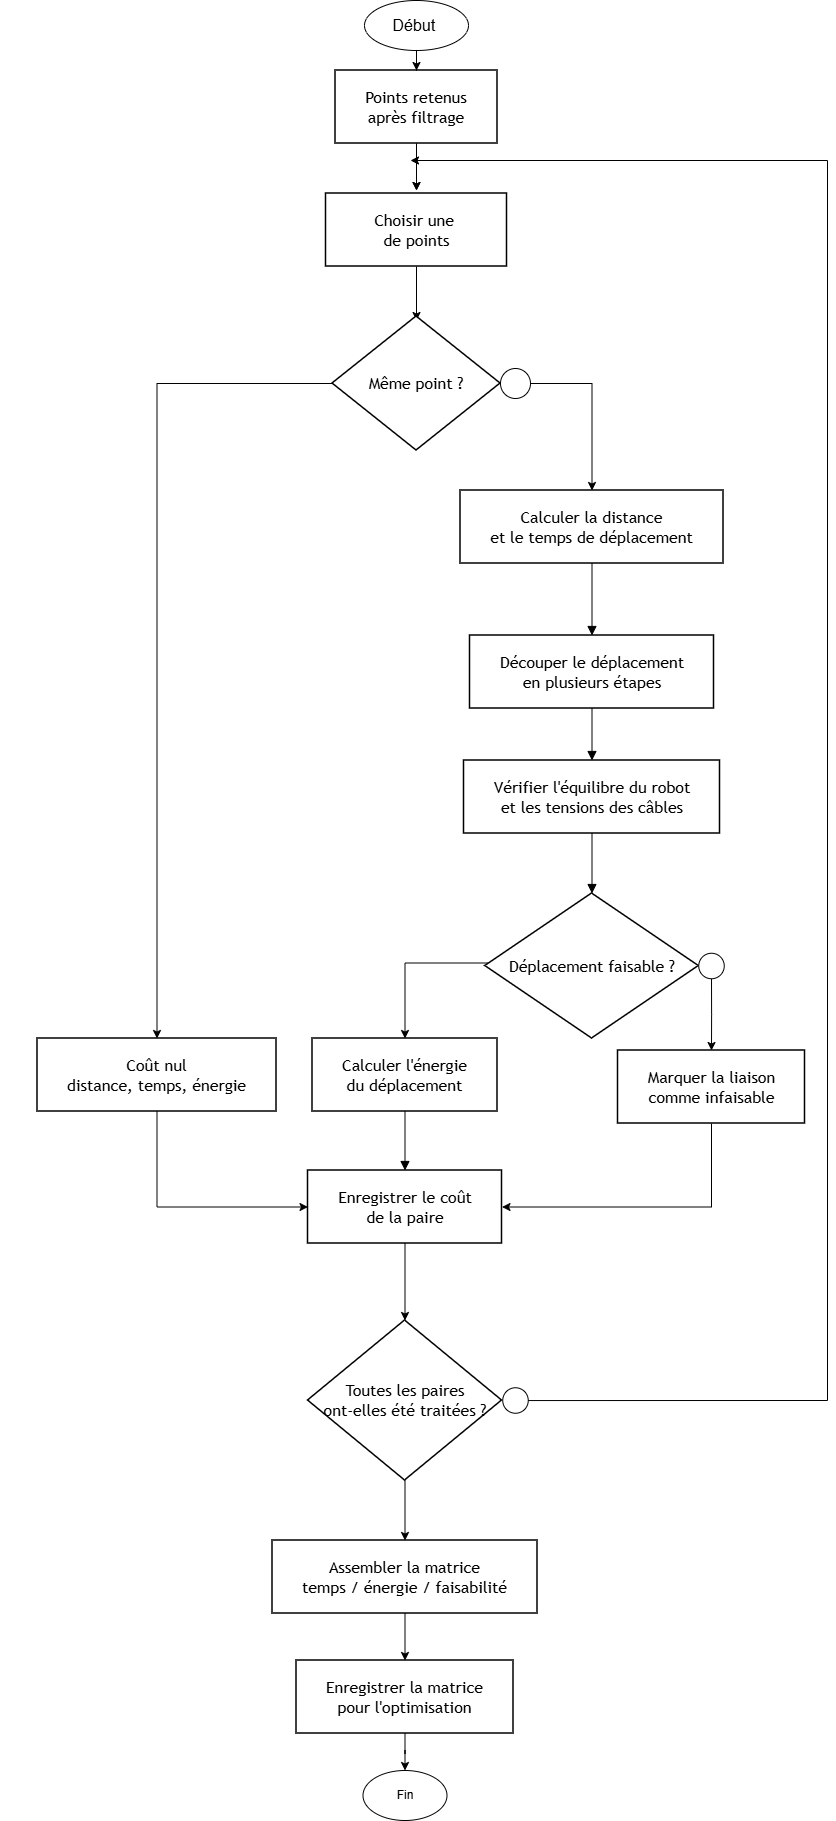
\includegraphics[width=\textwidth,height=0.82\textheight,keepaspectratio]{bloc6.png}
\caption{Organigramme du calcul de matrice de coût}
\label{fig:bloc6}
\end{figure}
\clearpage

Le temps de déplacement suit un profil LSPB :
\begin{equation}
d_{\mathrm{acc}}=\frac{v_{\max}^2}{2a_{\max}},\qquad d_{\mathrm{full}}=2\,d_{\mathrm{acc}}
\label{eq:dacc}
\end{equation}
Si $d\ge d_{\mathrm{full}}$, le profil est trapézoïdal ; sinon triangulaire. Avec $v_{\max}=0{,}045$~m/s et $a_{\max}=0{,}03$~m/s$^2$, $d_{\mathrm{acc}}\approx0{,}034$~m.

L'énergie est une estimation mécanique quasi-statique :
\begin{equation}
E\approx\sum_{k}\sum_{i=1}^{8}T_i\bigl(\mathbf{p}_k^{\mathrm{mid}}\bigr)\,|\Delta l_{i,k}|
\label{eq:energie}
\end{equation}
Les tensions sont obtenues par un QP à norme minimale, résolu d'abord par pseudo-inverse puis par SLSQP si nécessaire.

Un individu code une permutation des points non centraux. Les objectifs sont le temps et l'énergie totaux. Les contraintes sont gérées par pénalisation. NSGA-II utilise le croisement OX (taux 0,9) et la mutation par inversion (taux 0,1).

\subsection{Validation de la trajectoire}

Le sous-bloc~9 génère les profils LSPB ; le sous-bloc~10 contrôle sept invariants ; le sous-bloc~11 compare à une baseline. La mission suit six étapes : initialisation, déplacement, stabilisation 2~s, prise de vue, répétition, retour au centre.

\section{Préparation des données}

La campagne s'appuie sur une commande unique (grille, zero-loss, population, générations, graine~42). La graine rend l'optimisation déterministe. Pour la grille $7\times7$, le recouvrement entre points voisins assure une couverture complète de la parcelle.

\section{Génération de l'espace de travail}

\subsection{Zone sécurisée et frontière du WFW}

\begin{table}[H]
\centering
\caption{Synthèse de l'exploration de l'espace de travail}
\label{tab:wfw_synth}
\footnotesize
\begin{tabular}{|p{3.2cm}|c|c|c|c|c|}
\hline
\textbf{Configuration} & \textbf{Grille} & \textbf{Pas (m)} & \textbf{Bornes X/Y} & \textbf{Retenus} & \textbf{Taux} \\
\hline
Zone sécurisée & $7\times7$ & $0{,}133\times0{,}080$ & $\pm0{,}40/\pm0{,}24$ & 49/49 & 100~\% \\
\hline
Zone sécurisée & $9\times9$ & $0{,}100\times0{,}060$ & $\pm0{,}40/\pm0{,}24$ & 81/81 & 100~\% \\
\hline
Zone étendue & $7\times7$ & $0{,}150\times0{,}090$ & $\pm0{,}45/\pm0{,}27$ & 49/49 & 100~\% \\
\hline
Zone étendue & $9\times9$ & $0{,}150\times0{,}090$ & $\pm0{,}60/\pm0{,}36$ & 77/81 & 95,1~\% \\
\hline
\end{tabular}
\end{table}

\begin{figure}[H]
\centering
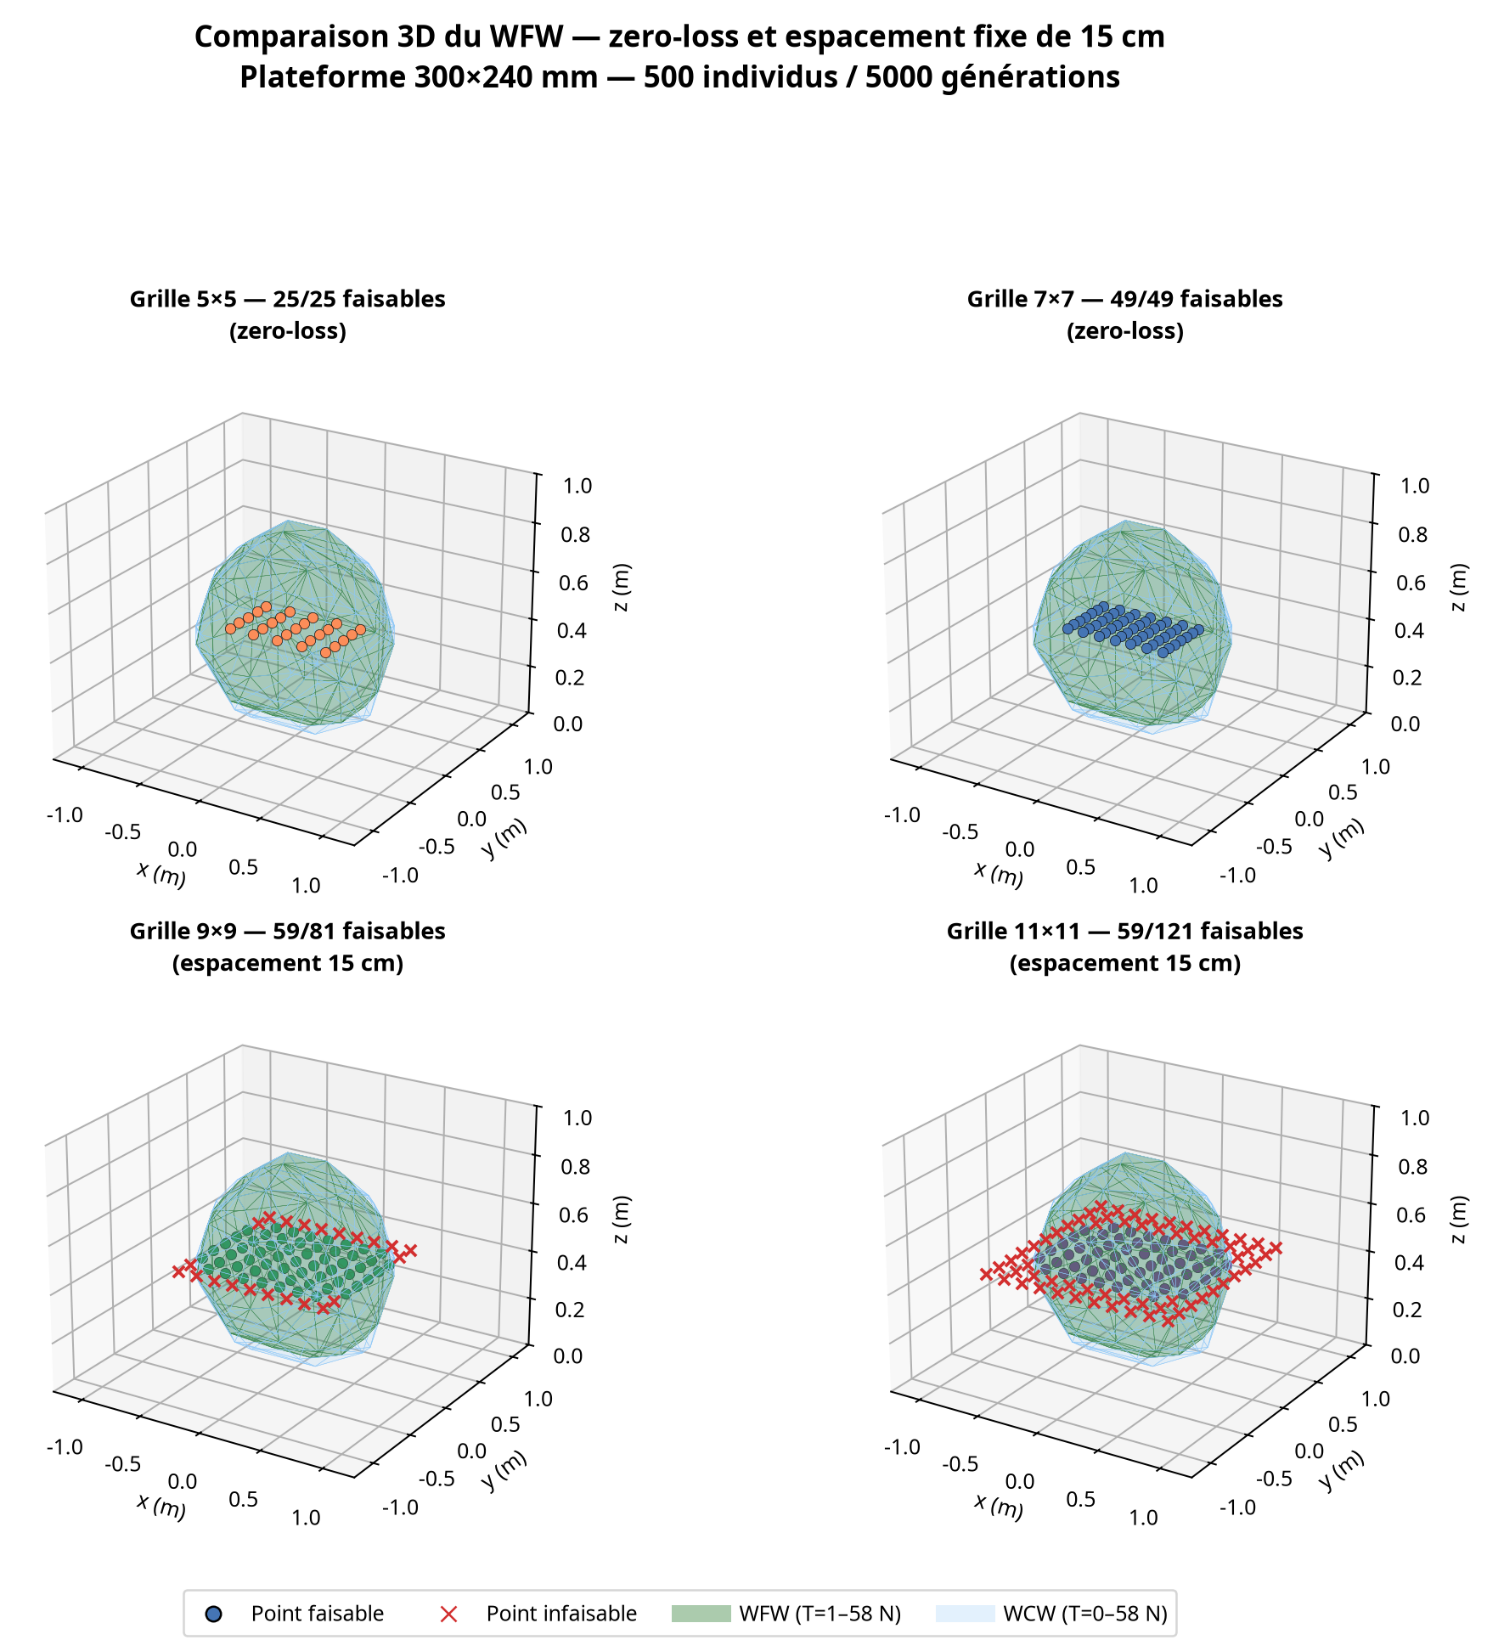
\includegraphics[width=0.95\textwidth,height=0.48\textheight,keepaspectratio]{wfw_grille.jpg}
\caption{WFW 3D et faisabilité des points selon la taille de grille}
\label{fig:wfw_grille}
\end{figure}

L'espace de travail faisable en effort (WFW) présente une forme sphérique tronquée dont les limites physiques rejettent les points situés aux extrémités de la grille (croix rouges). Ce comportement justifie le recours au mode «~zero-loss~» : pour garantir 100~\% de points viables, la zone de travail doit être volontairement restreinte.


\section{Optimisation des trajectoires : dimensionnement de NSGA-II}

Campagne de 50 exécutions (2 grilles $\times$ 5 populations $\times$ 5 générations), graine~42, complétée par 12 exécutions de robustesse (graines 30 et 100).

\begin{table}[H]
\centering
\caption{Grille $7\times7$ : temps (s) / énergie (J) du meilleur point, graine 42}
\label{tab:camp7}
\footnotesize
\begin{tabular}{|c|c|c|c|c|c|}
\hline
\textbf{Pop.} & \textbf{1500} & \textbf{2000} & \textbf{3000} & \textbf{4000} & \textbf{5000} \\
\hline
200 & 178,58 / 248,8 & 177,98 / 247,1 & 177,98 / 247,0 & 177,98 / 247,0 & 177,98 / 247,0 \\
\hline
300 & 177,30 / 246,4 & 177,30 / 246,4 & 177,30 / 246,4 & 177,30 / 246,4 & 177,30 / 246,4 \\
\hline
400 & 178,96 / 250,4 & 177,98 / 248,1 & 177,98 / 247,5 & 177,98 / 247,0 & 177,30 / 246,7 \\
\hline
500 & 177,30 / 246,4 & 177,30 / 246,4 & 177,30 / 246,4 & 177,30 / 246,4 & 177,30 / 246,4 \\
\hline
600 & 177,30 / 246,4 & 177,30 / 246,4 & 177,30 / 246,4 & 177,30 / 246,4 & 177,30 / 246,4 \\
\hline
\end{tabular}
\end{table}

\begin{table}[H]
\centering
\caption{Grille $9\times9$ : temps (s) / énergie (J) du meilleur point, graine 42}
\label{tab:camp9}
\footnotesize
\begin{tabular}{|c|c|c|c|c|c|}
\hline
\textbf{Pop.} & \textbf{1500} & \textbf{2000} & \textbf{3000} & \textbf{4000} & \textbf{5000} \\
\hline
200 & 267,17 / 325,4 & 262,20 / 318,8 & 255,64 / 307,4 & 254,90 / 304,3 & 253,65 / 304,3 \\
\hline
300 & 260,02 / 312,4 & 253,57 / 304,7 & 248,60 / 295,2 & 248,09 / 295,2 & 247,55 / 294,2 \\
\hline
400 & 262,77 / 315,6 & 253,77 / 304,3 & 252,06 / 301,7 & 249,98 / 299,0 & 249,98 / 297,9 \\
\hline
500 & 248,09 / 296,6 & 248,09 / 296,6 & 247,55 / 295,6 & 247,04 / 295,4 & 247,04 / 294,8 \\
\hline
600 & 255,44 / 310,2 & 253,90 / 305,5 & 249,81 / 298,0 & 247,78 / 294,1 & 247,04 / 294,1 \\
\hline
\end{tabular}
\end{table}

\begin{figure}[H]
\centering
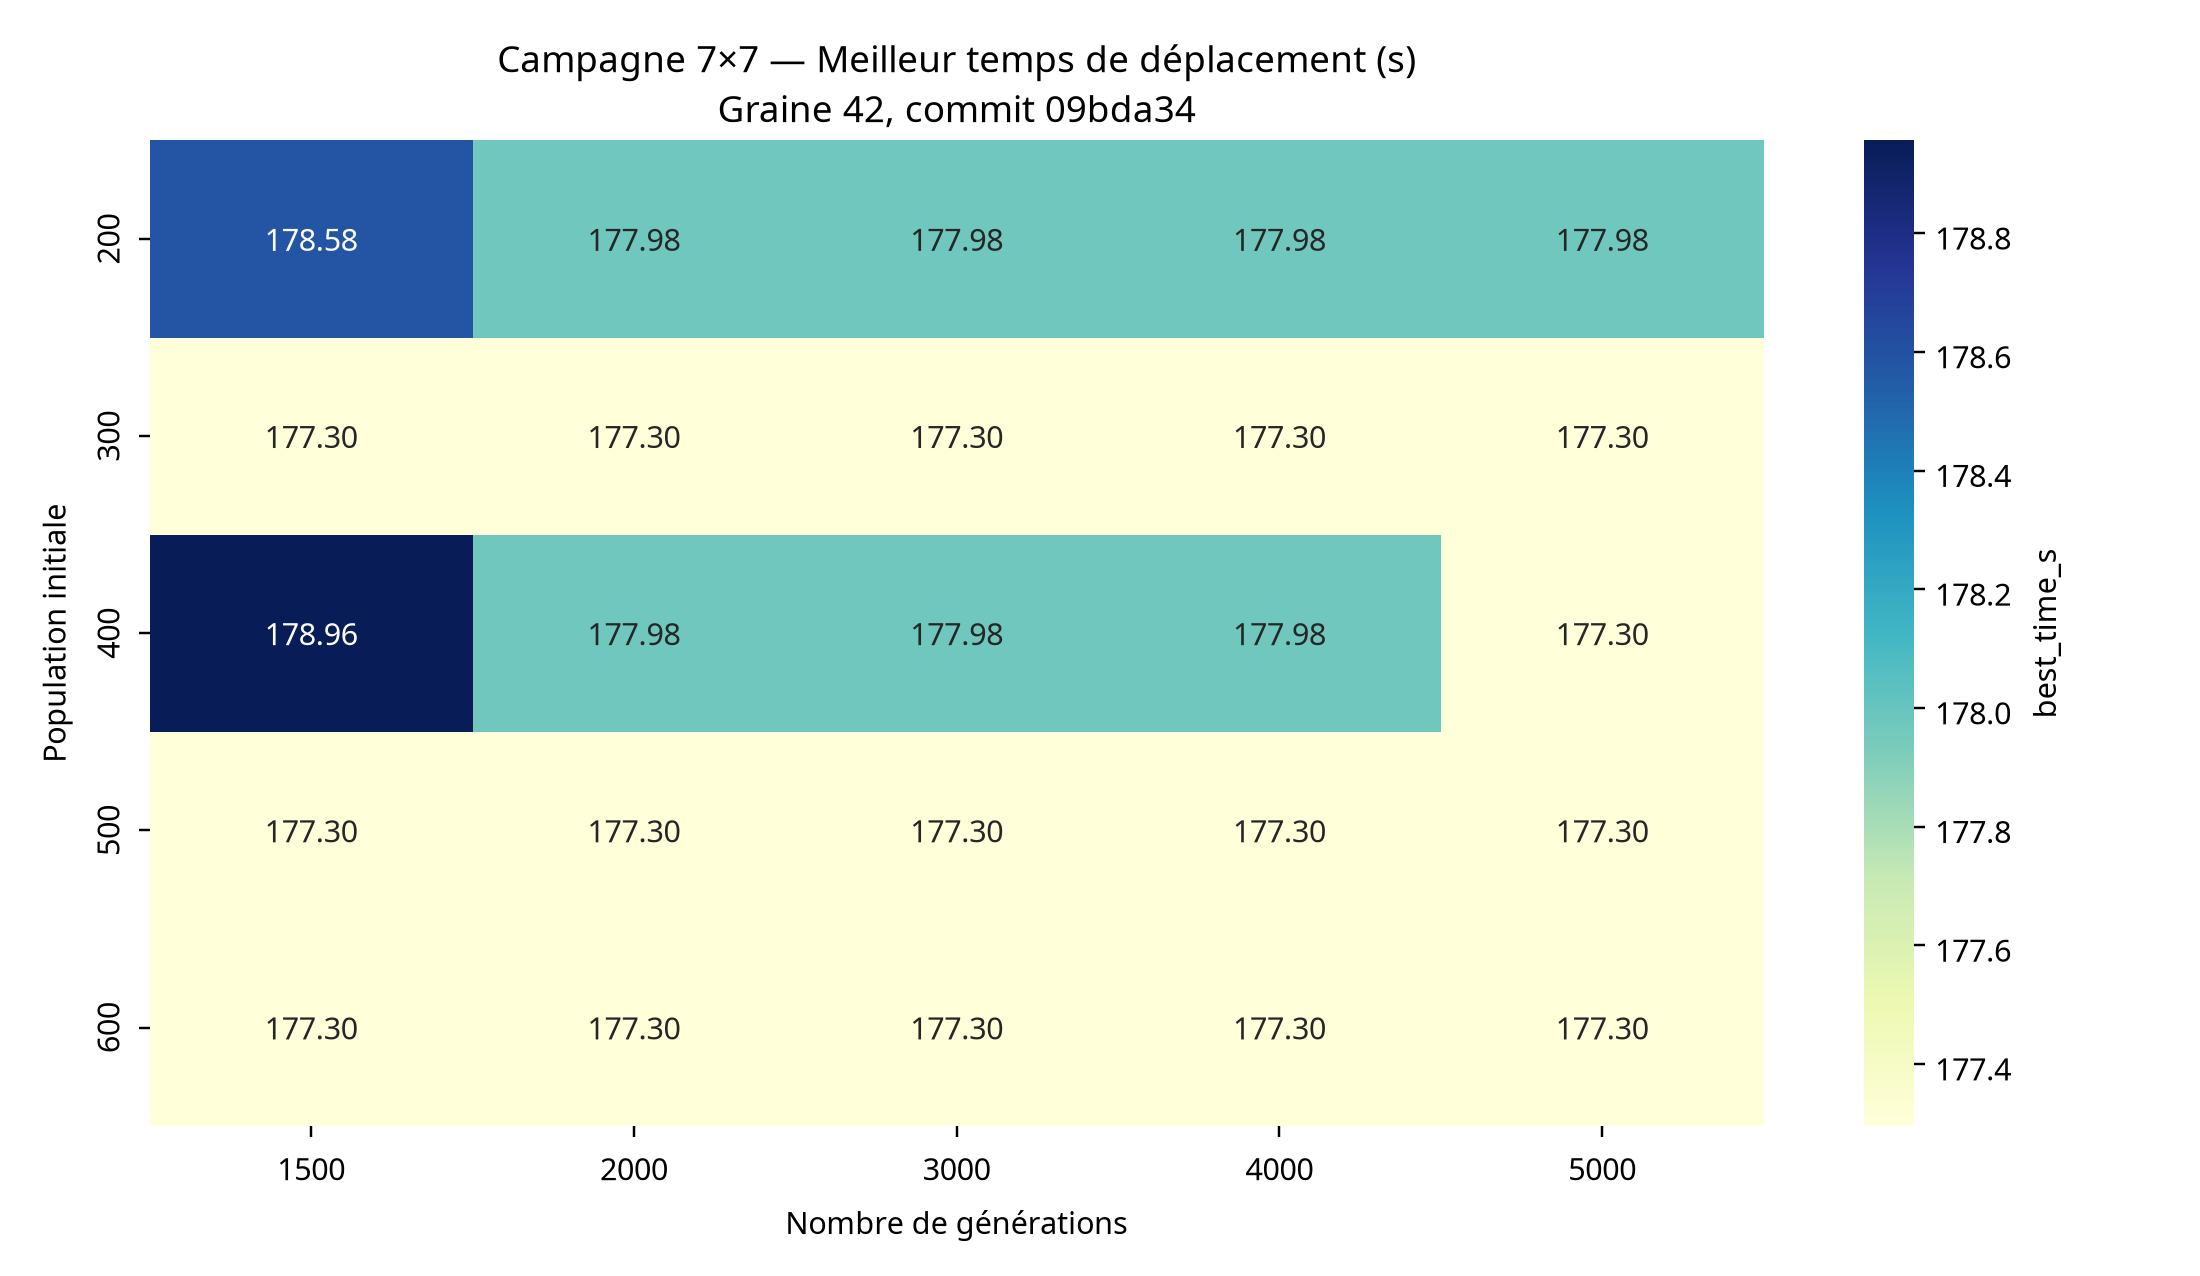
\includegraphics[width=0.92\textwidth,height=0.34\textheight,keepaspectratio]{hm_time_7x7.png}\\[0.3em]
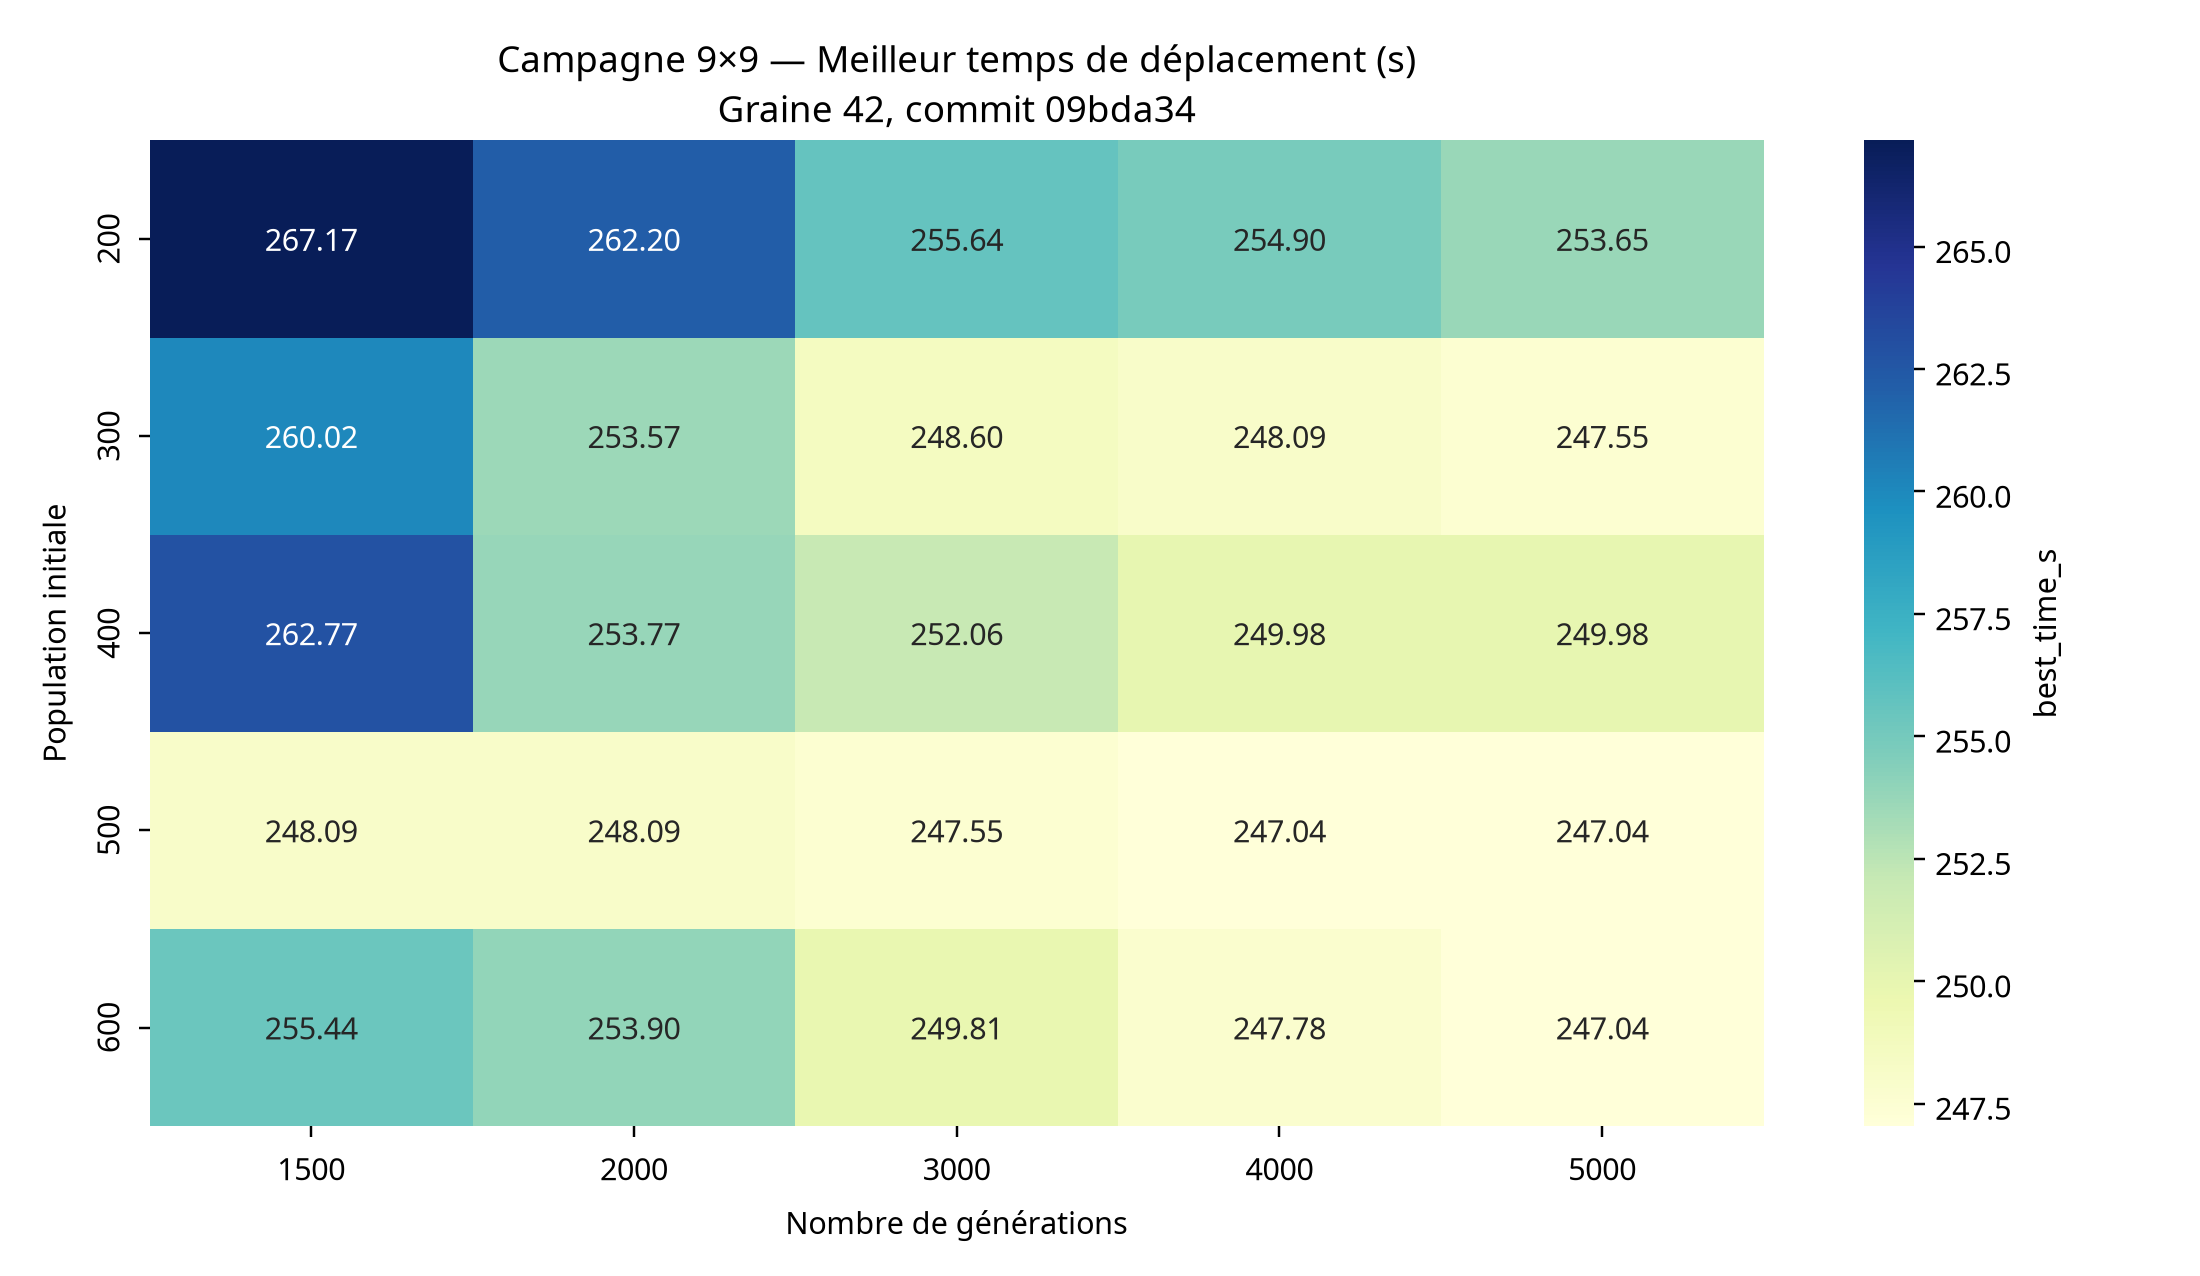
\includegraphics[width=0.92\textwidth,height=0.34\textheight,keepaspectratio]{hm_time_9x9.png}
\caption{Cartes de chaleur du meilleur temps : (a) grille $7\times7$, (b) grille $9\times9$}
\label{fig:hm_time}
\end{figure}

La convergence du temps de déplacement dépend fortement de la taille de la grille. Alors que le plateau optimal est atteint dès 1500 générations pour la grille $7\times7$, il faut attendre 5000 générations pour stabiliser la grille $9\times9$. Cela justifie le dimensionnement différencié des paramètres de NSGA-II retenu pour chaque configuration.


\begin{figure}[H]
\centering
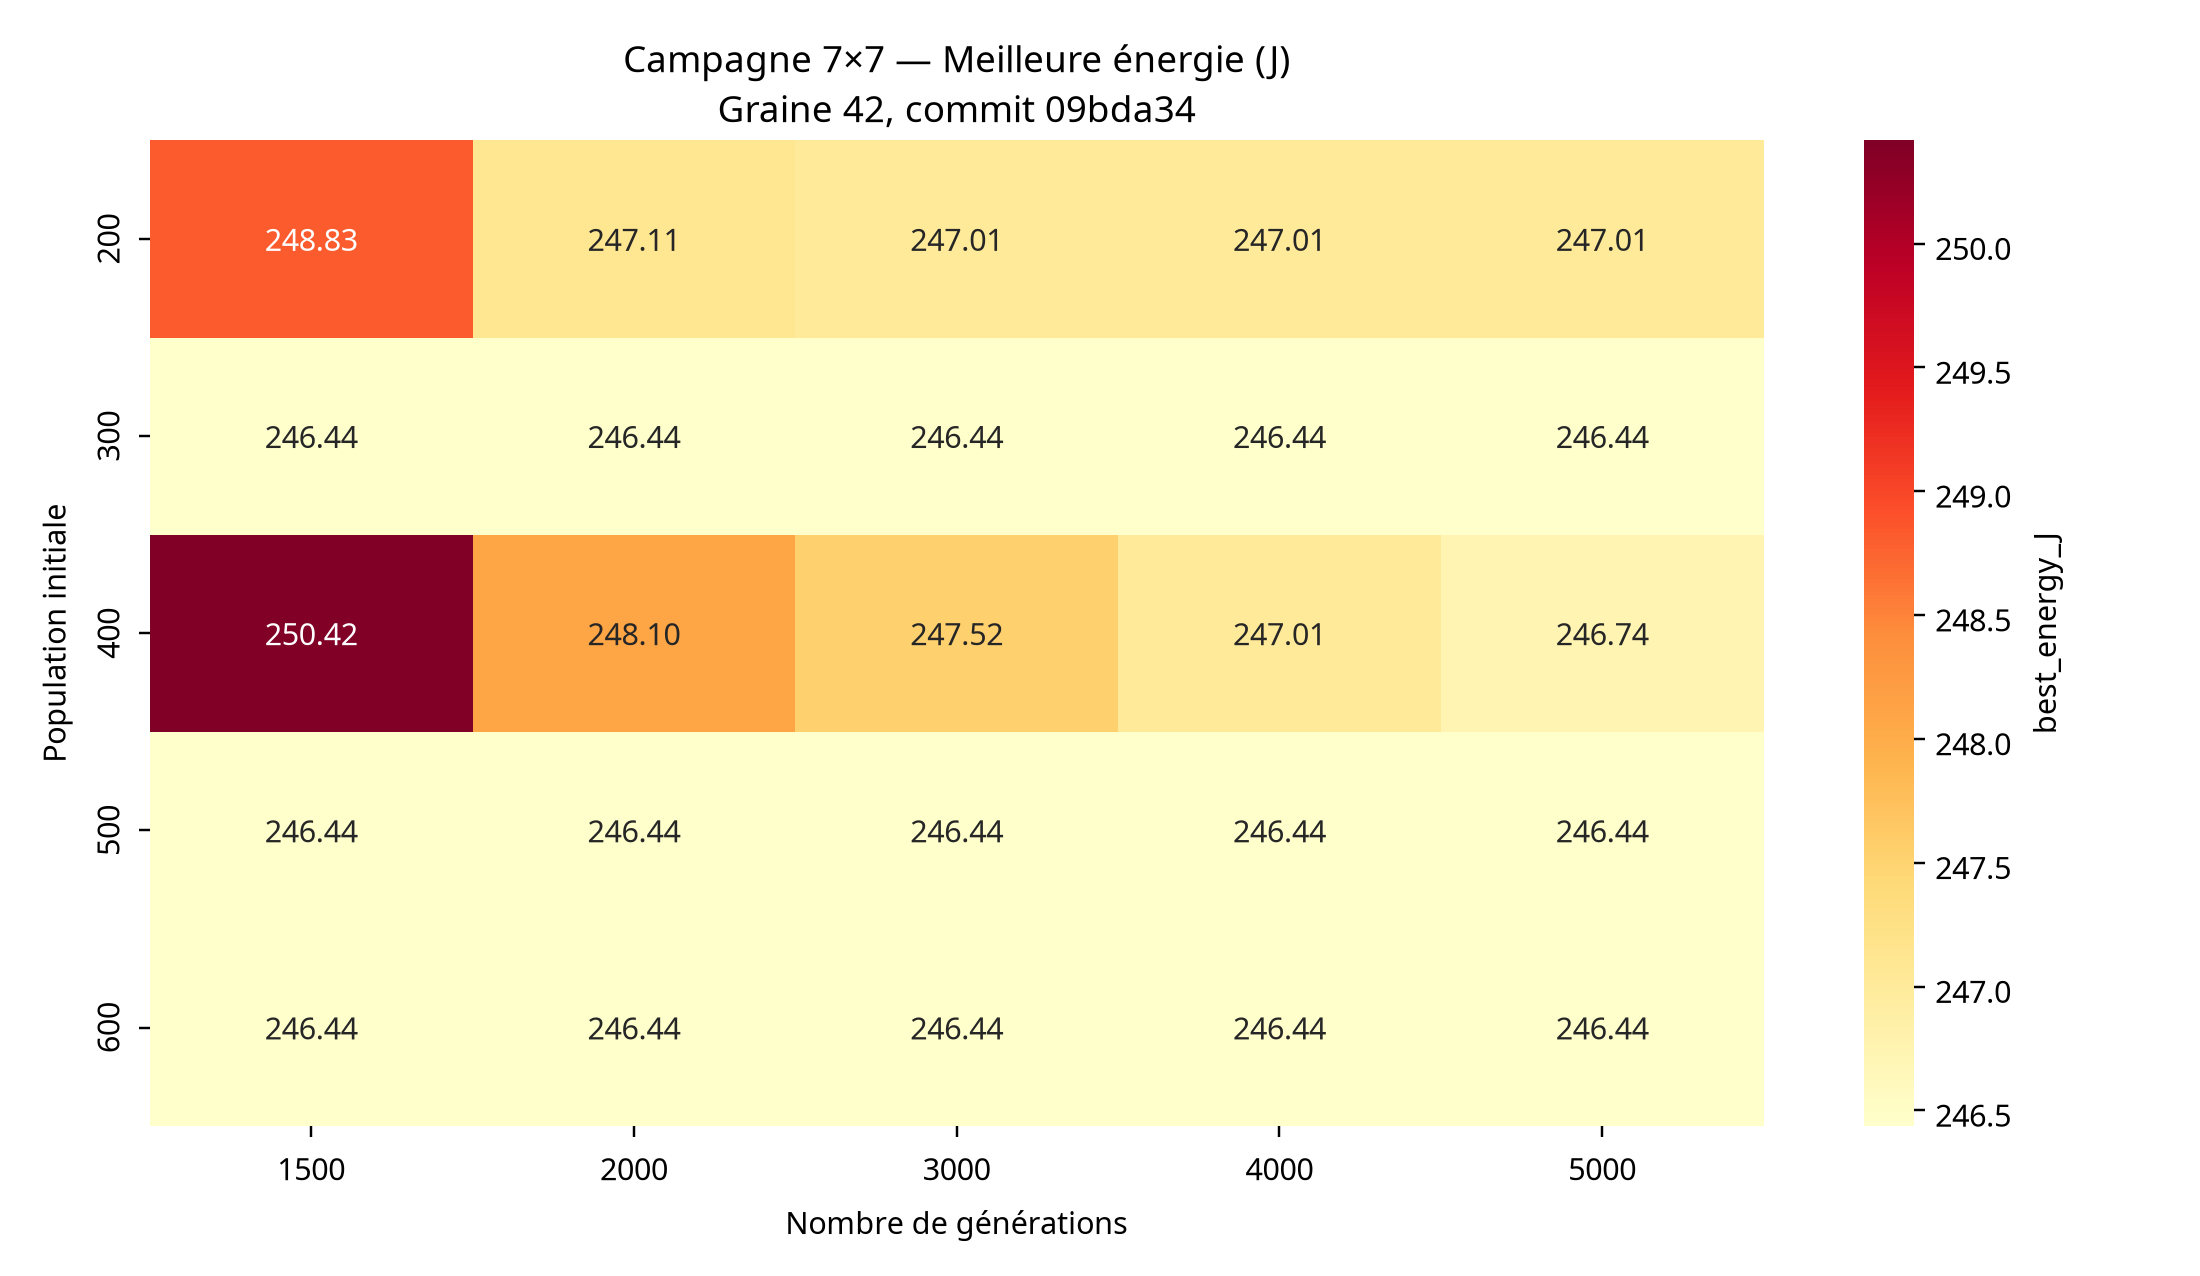
\includegraphics[width=0.92\textwidth,height=0.34\textheight,keepaspectratio]{hm_energy_7x7.png}\\[0.3em]
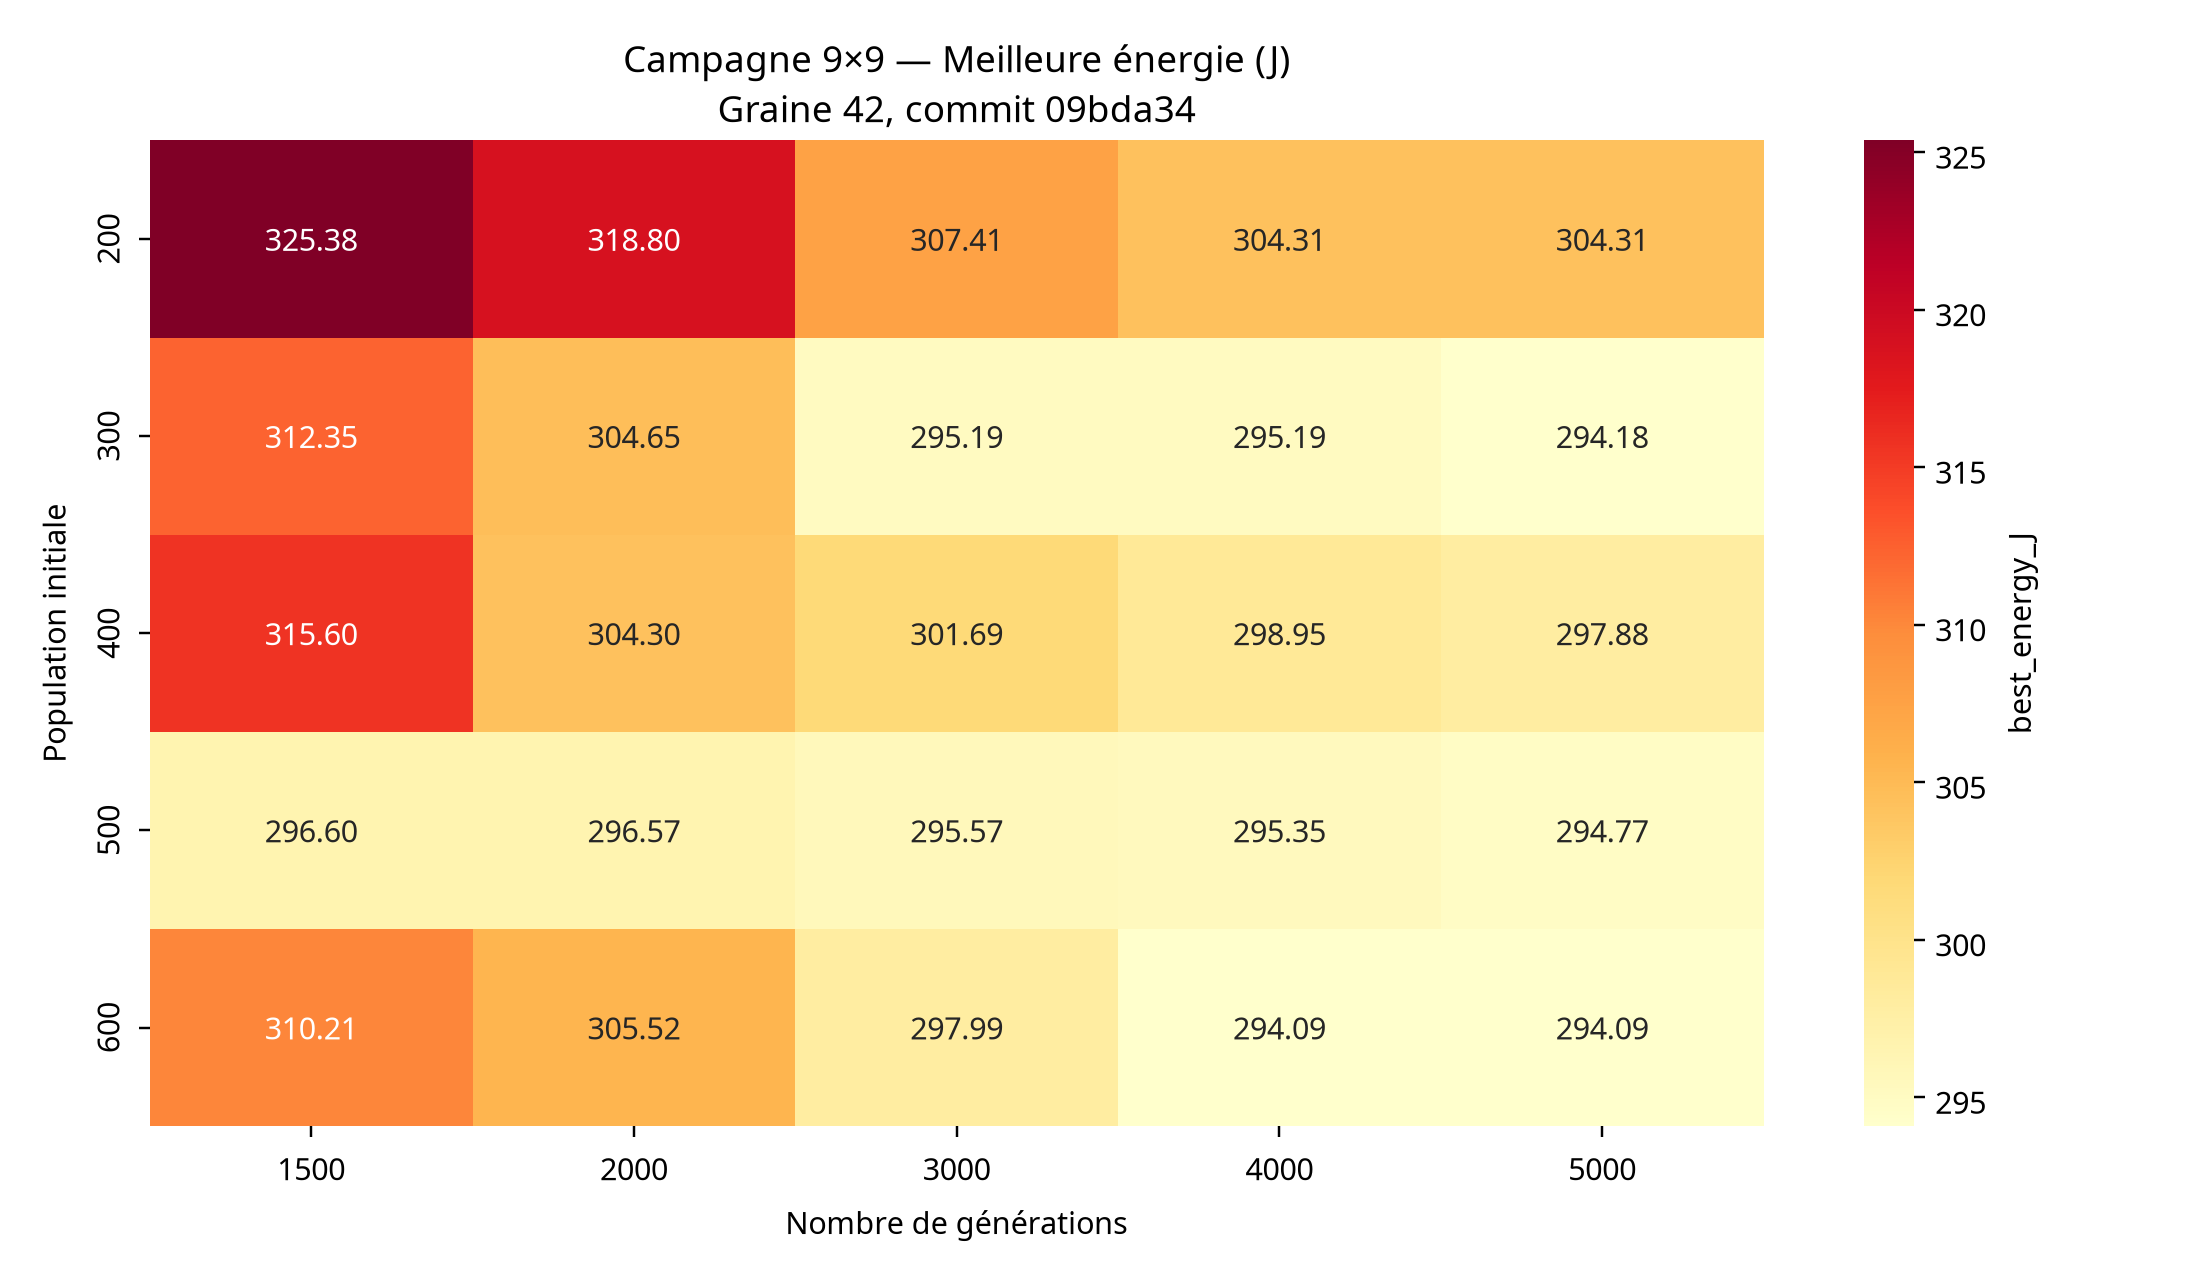
\includegraphics[width=0.92\textwidth,height=0.34\textheight,keepaspectratio]{hm_energy_9x9.png}
\caption{Cartes de chaleur de la meilleure énergie : (a) grille $7\times7$, (b) grille $9\times9$}
\label{fig:hm_energy}
\end{figure}



\begin{table}[H]
\centering
\caption{Robustesse sur trois graines (42, 30 et 100)}
\label{tab:robust}
\footnotesize
\begin{tabular}{|c|c|c|c|c|}
\hline
\textbf{Grille} & \textbf{Pop. $\times$ gén.} & \textbf{Temps $\pm\sigma$ (s)} & \textbf{Énergie $\pm\sigma$ (J)} & \textbf{Durée (s)} \\
\hline
$7\times7$ & $300\times1500$ & $178{,}31\pm0{,}89$ & $248{,}5\pm2{,}1$ & 37 \\
\hline
$7\times7$ & $500\times2000$ & $177{,}98\pm0{,}69$ & $247{,}4\pm1{,}1$ & 73 \\
\hline
$7\times7$ & $600\times3000$ & $177{,}52\pm0{,}39$ & $246{,}6\pm0{,}3$ & 132 \\
\hline
$9\times9$ & $500\times5000$ & $248{,}65\pm2{,}79$ & $295{,}9\pm3{,}2$ & 205 \\
\hline
$9\times9$ & $600\times4000$ & $247{,}44\pm0{,}39$ & $293{,}5\pm1{,}2$ & 211 \\
\hline
$9\times9$ & $600\times5000$ & $247{,}02\pm0{,}51$ & $293{,}3\pm1{,}2$ & 248 \\
\hline
\end{tabular}
\end{table}

\begin{figure}[H]
\centering
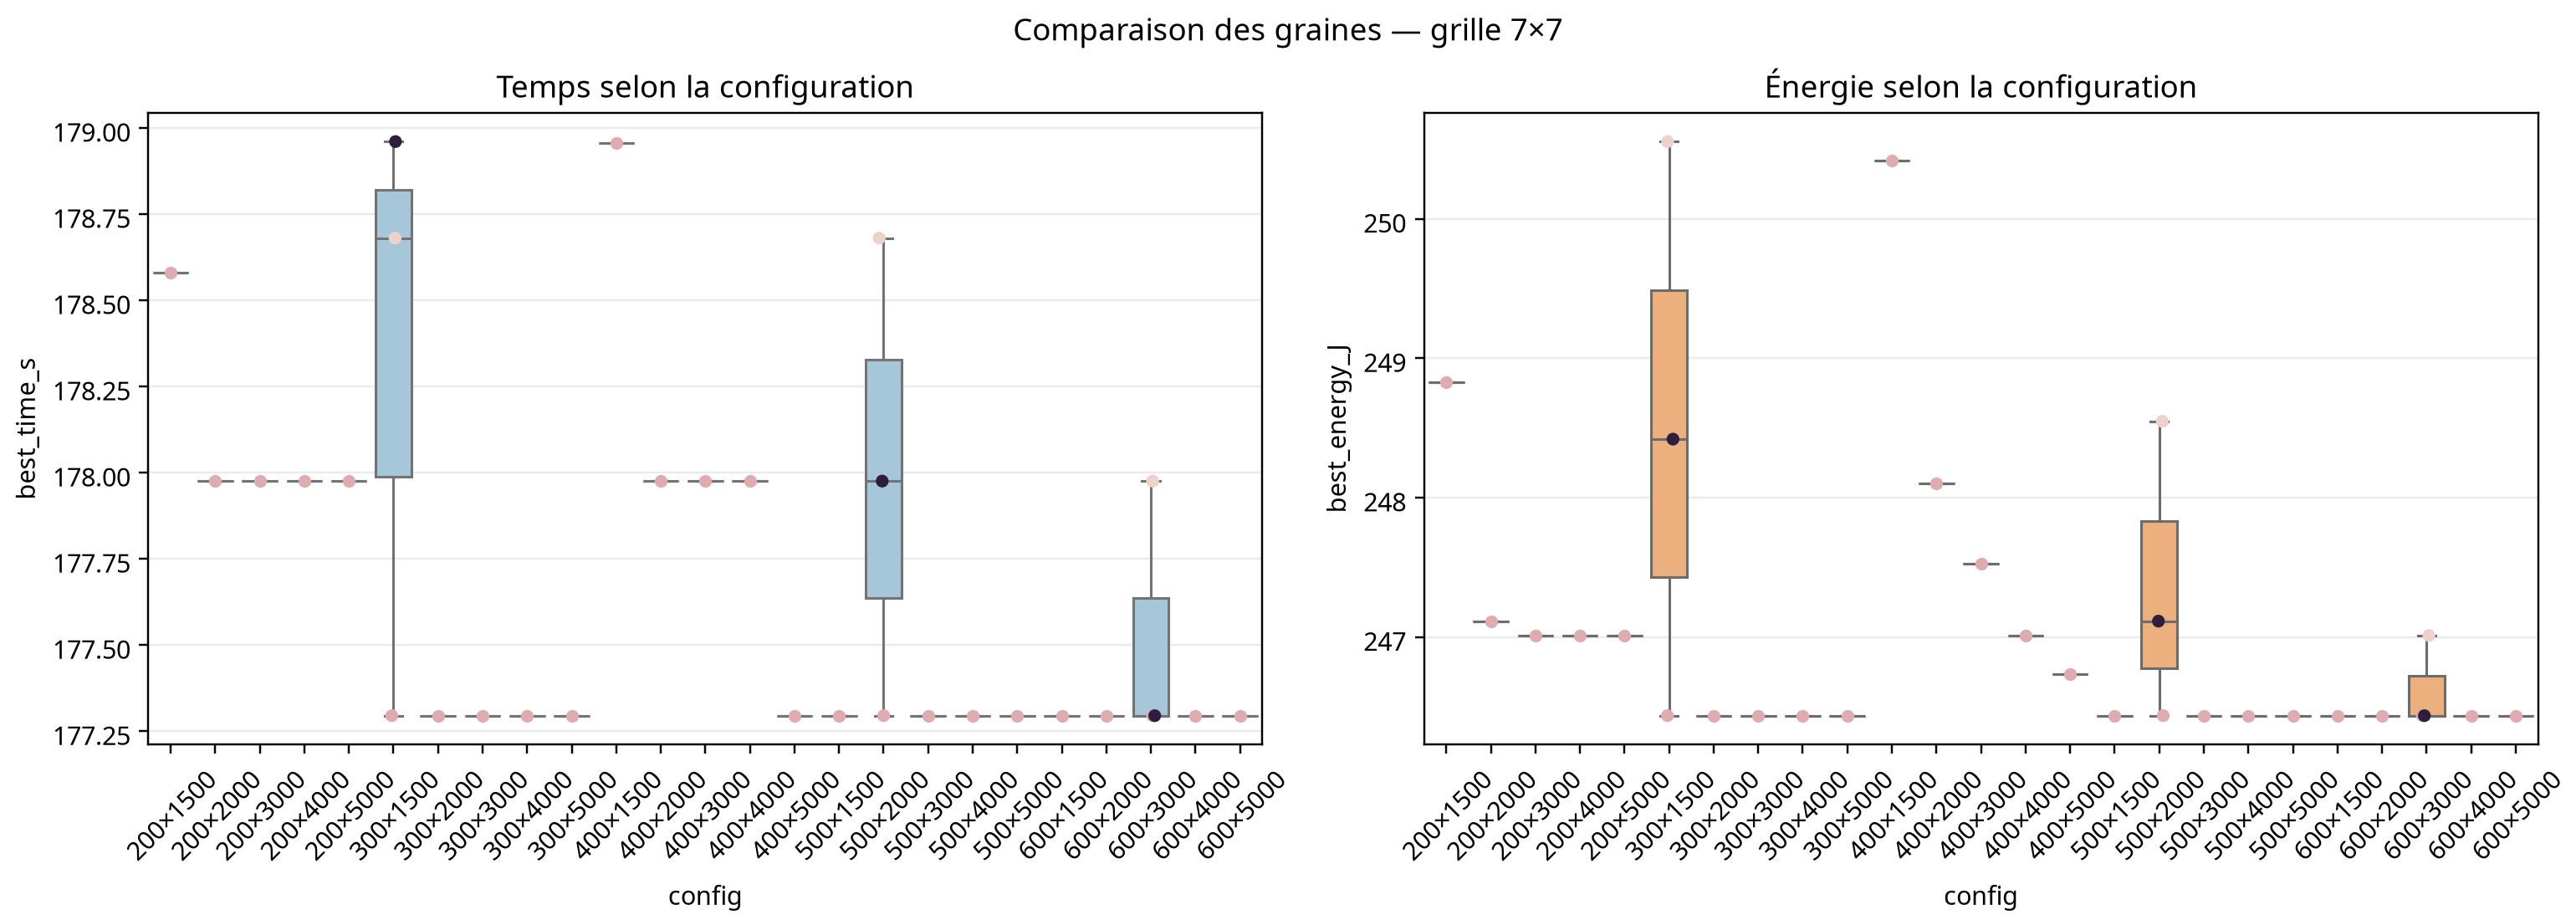
\includegraphics[width=0.92\textwidth,height=0.28\textheight,keepaspectratio]{robust_box_7x7.png}
\caption{Dispersion du temps et de l'énergie selon la configuration (grille $7\times7$)}
\label{fig:robust_box}
\end{figure}

L'analyse de la dispersion sur 50 exécutions révèle une réduction drastique de la variabilité (boîtes plus courtes, disparition des valeurs aberrantes) lorsque la taille de la population augmente. Une population de 500 individus garantit ainsi une stabilité et une reproductibilité accrues de l'algorithme, indépendamment du hasard.


\begin{figure}[H]
\centering
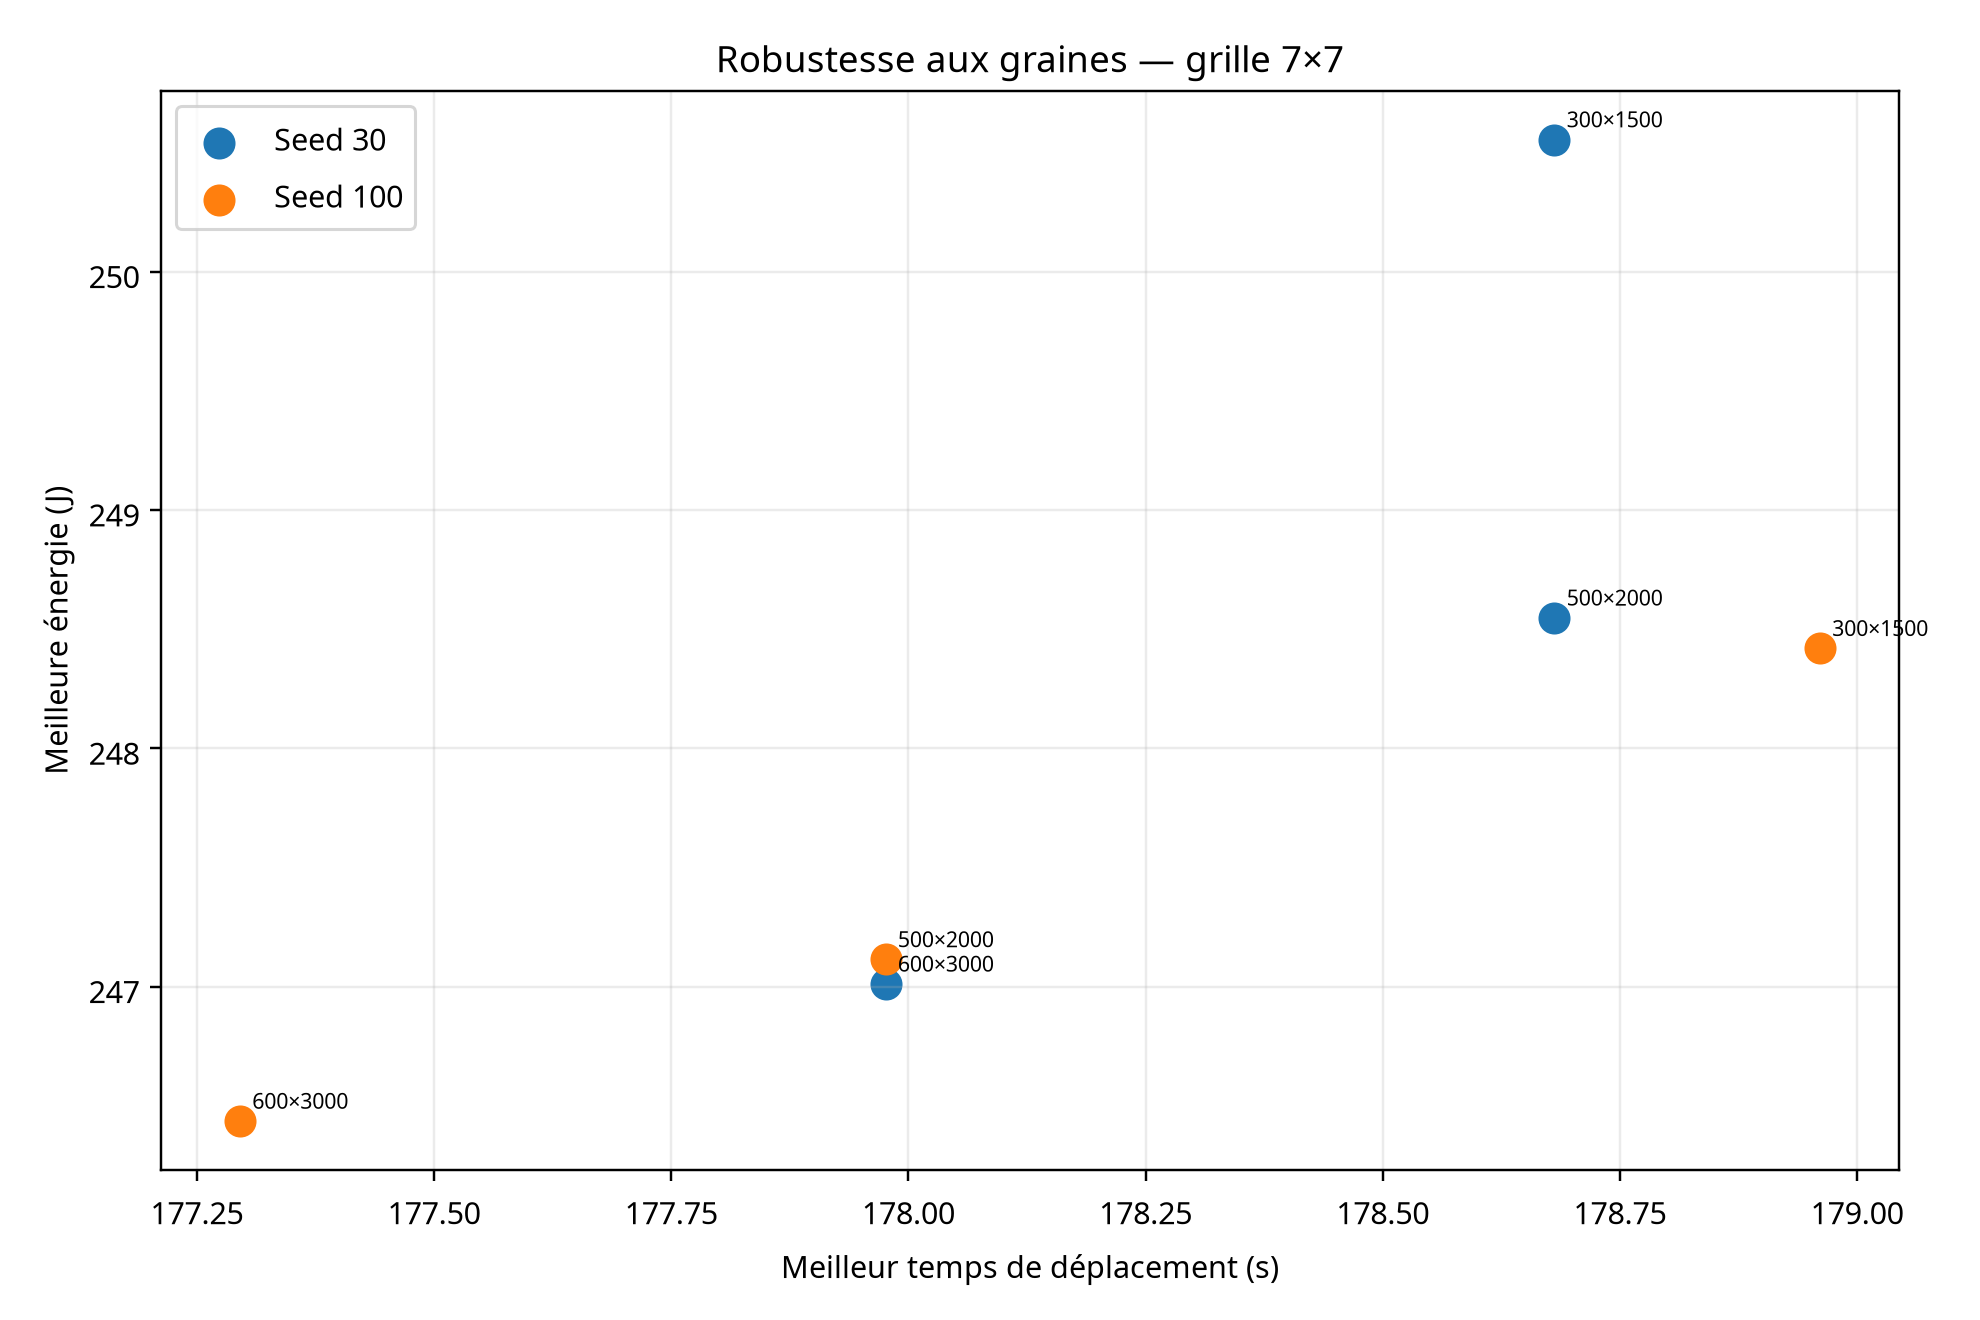
\includegraphics[width=0.90\textwidth,height=0.26\textheight,keepaspectratio]{robust_seeds_7x7.png}\\[0.2em]
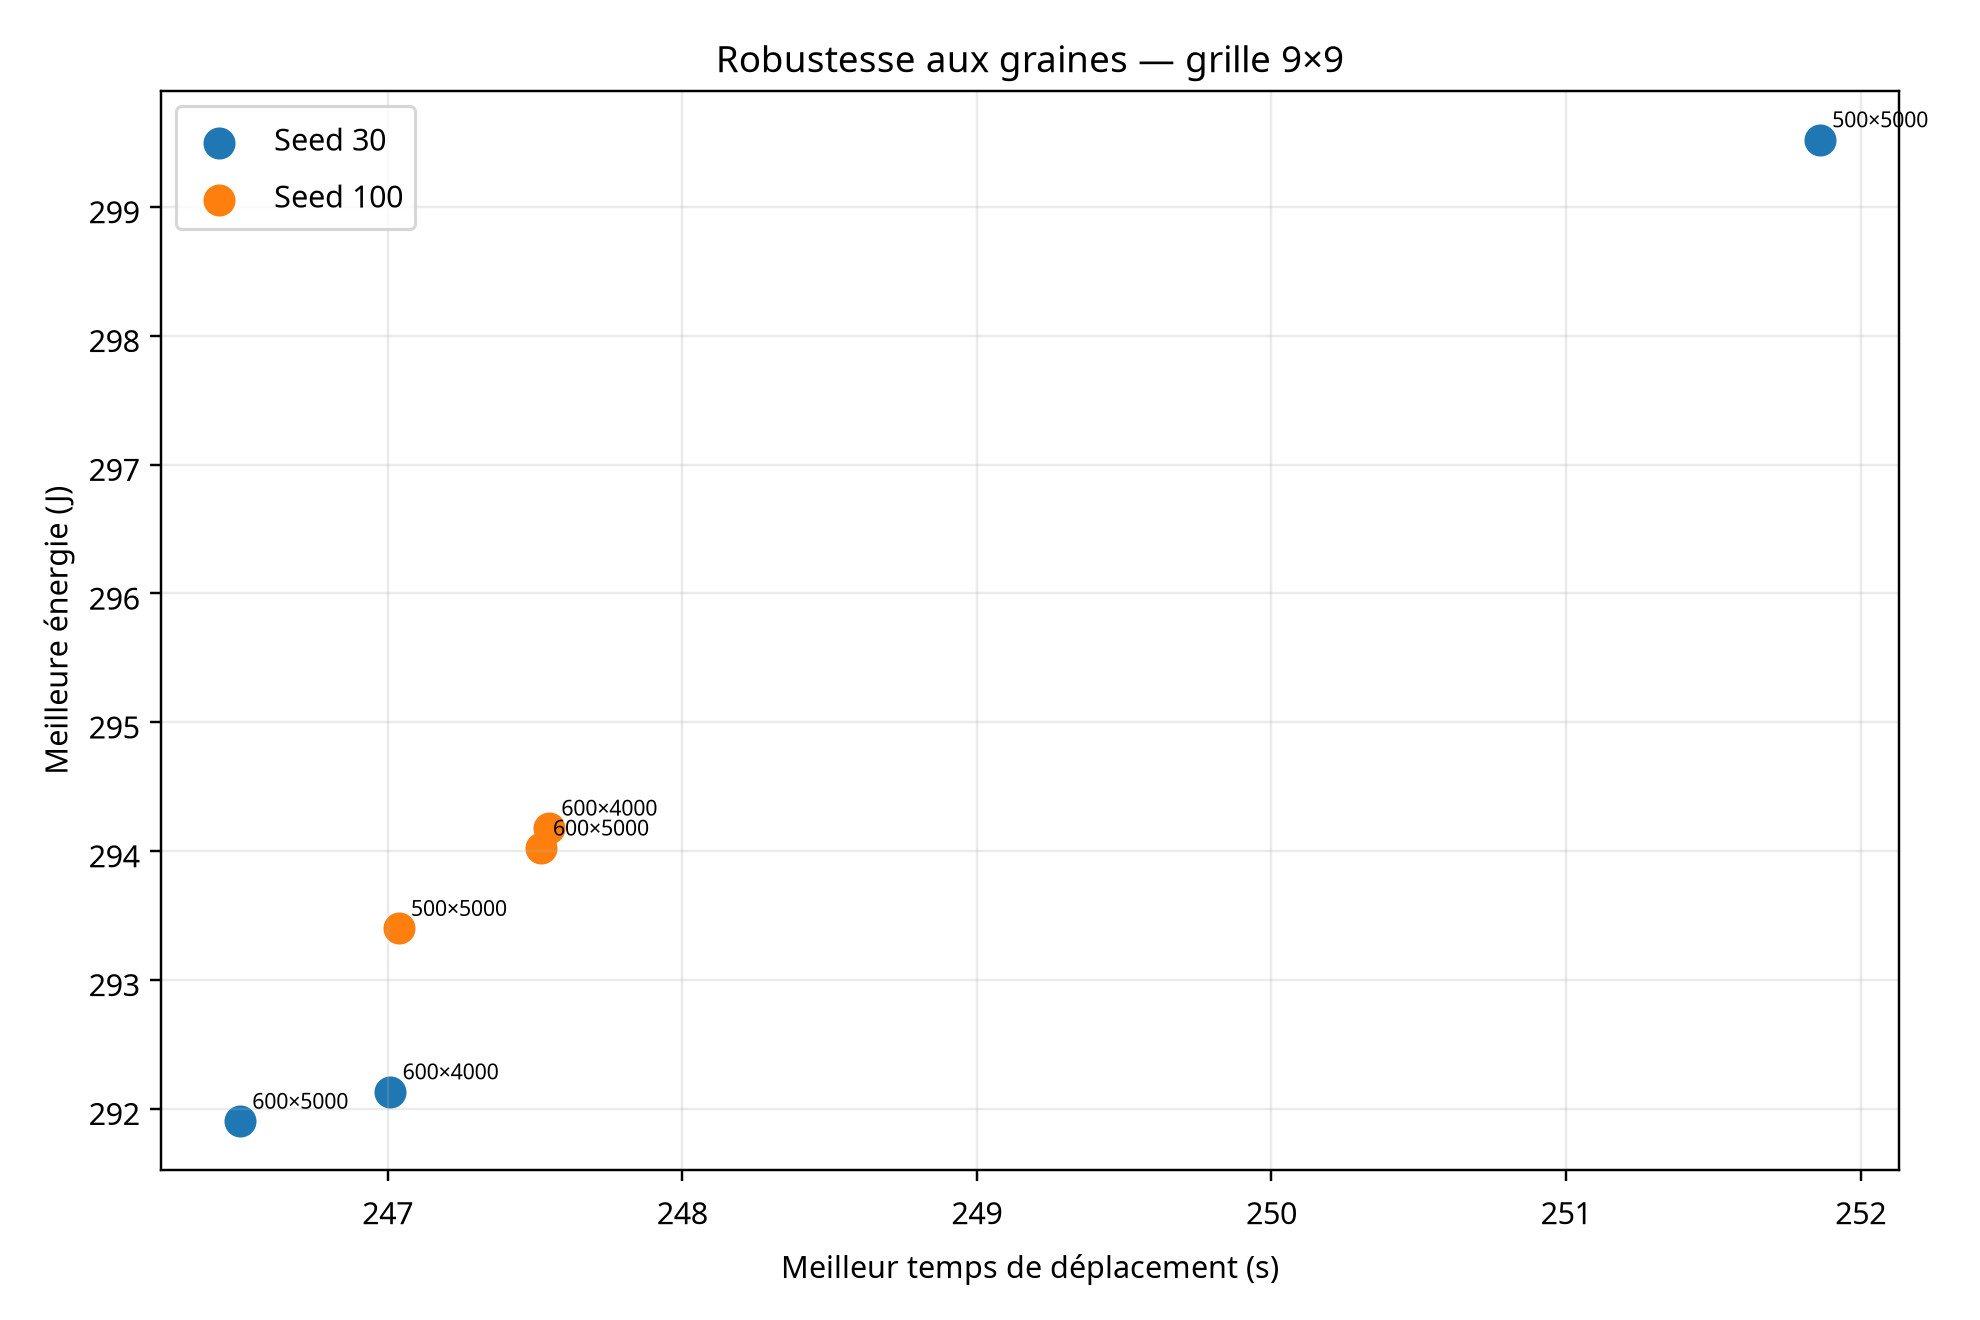
\includegraphics[width=0.90\textwidth,height=0.26\textheight,keepaspectratio]{robust_seeds_9x9.png}
\caption{Positions des graines 30 et 100 dans le plan temps--énergie}
\label{fig:robust_seeds}
\end{figure}

La comparaison des graines aléatoires (30 et 100) montre un regroupement spatial très serré des solutions dans l'espace des objectifs. Cette convergence démontre la robustesse statistique de NSGA-II : la qualité de la trajectoire optimisée ne dépend pas d'un «~coup de chance~», mais converge systématiquement vers les meilleures performances.


\begin{table}[H]
\centering
\caption{Paramètres retenus}
\label{tab:params}
\begin{tabular}{|c|c|c|p{7cm}|}
\hline
\textbf{Grille} & \textbf{Population} & \textbf{Générations} & \textbf{Justification} \\
\hline
$7\times7$ & 500 & 2000 & Meilleur résultat graine 42 en 73~s, dispersion modérée \\
\hline
$9\times9$ & 600 & 5000 & Meilleure moyenne (247,02~s ; 293,3~J), dispersion faible \\
\hline
\end{tabular}
\end{table}

\section{Vérification numérique}
\label{sec:verif}

\begin{table}[H]
\centering
\caption{Résultats de validation du run de référence $7\times7$}
\label{tab:valid}
\footnotesize
\begin{tabular}{|p{5cm}|c|p{7cm}|}
\hline
\textbf{Invariant} & \textbf{Statut} & \textbf{Évidence} \\
\hline
Cohérence de la configuration & PASS & $N=49$ ; $T\in[1;58]$~N ; orientation fixe \\
\hline
Faisabilité des points filtrés & PASS & 49 points ; aucun infaisable \\
\hline
Symétrie de la matrice de coûts & PASS & 2401 entrées ; symétrie ; diagonale nulle \\
\hline
Non-dominance (front de Pareto) & WARN & Une solution non dominée unique \\
\hline
Cohérence des trajectoires & PASS & 3 types ; centre aux extrémités \\
\hline
Profils cinématiques & PASS & 5361 échantillons ; $v_{\max}=0{,}045$~m/s \\
\hline
Cohérence croisée & PASS & Profils, matrice et résumé concordants \\
\hline
\end{tabular}
\end{table}

Résultat : 6 PASS, 1 WARN, 0 FAIL sur les 50 exécutions. Le WARN signale un front trop réduit pour étudier le compromis temps--énergie.

\section{Résultats et analyse}

\subsection{Configuration de référence (zone sécurisée)}

Pour la grille $7\times7$ : solution unique 177,30~s / 246,44~J contre baseline 229,3~s / 340,3~J (gains 22,7~\% et 27,6~\%). Pour la grille $9\times9$ : temps minimal 247,04~s, énergie minimale 294,09~J contre baseline 312,9~s / 412,6~J (gains 21,0~\% et 28,7~\%).

\begin{table}[H]
\centering
\caption{Résultats de la configuration de référence}
\label{tab:res_ref}
\footnotesize
\begin{tabular}{|c|c|c|c|c|c|c|c|}
\hline
\textbf{Grille} & \textbf{Temps (s)} & \textbf{Énergie (J)} & \textbf{Baseline} & \textbf{Gain t} & \textbf{Gain E} & \textbf{Stab.} & \textbf{Total} \\
\hline
$7\times7$ & 177,30 & 246,44 & 229,3 / 340,3 & 22,7~\% & 27,6~\% & 98~s & 275,3~s \\
\hline
$9\times9$ & 247,04 & 294,09 & 312,9 / 412,6 & 21,0~\% & 28,7~\% & 162~s & 409,0~s \\
\hline
\end{tabular}
\end{table}

\begin{figure}[H]
\centering
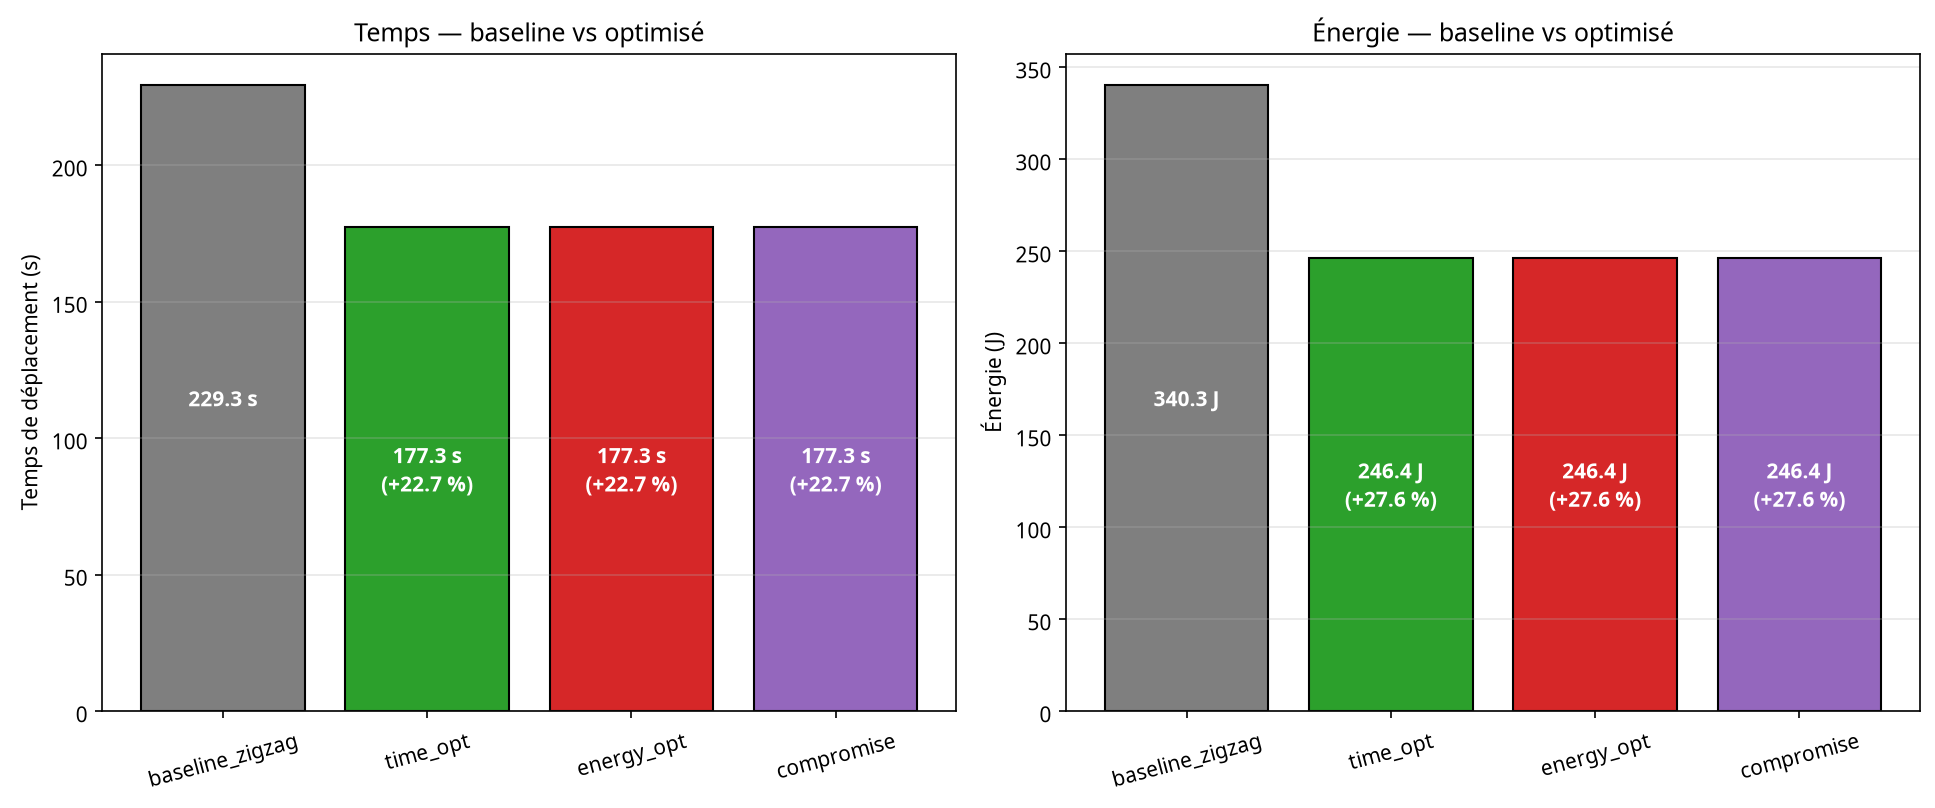
\includegraphics[width=0.92\textwidth,height=0.34\textheight,keepaspectratio]{comp_sec_7x7.png}\\[0.3em]
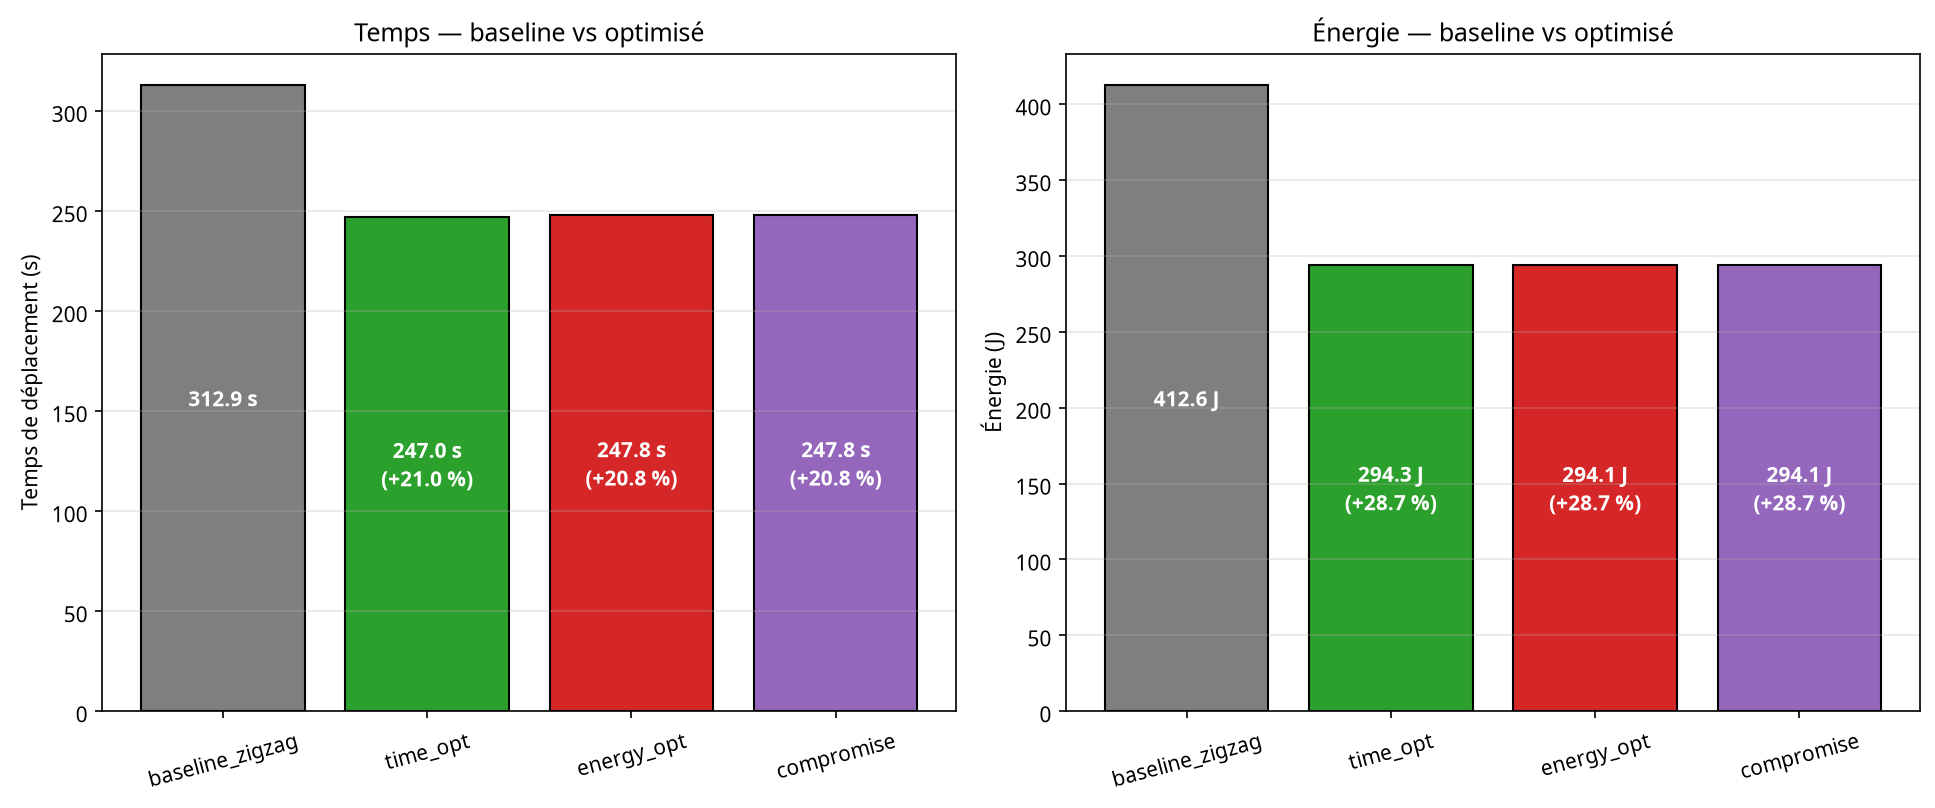
\includegraphics[width=0.92\textwidth,height=0.34\textheight,keepaspectratio]{comp_sec_9x9.png}
\caption{Temps et énergie : baseline zigzag et trajectoires optimisées, zone sécurisée}
\label{fig:comp_sec}
\end{figure}

La comparaison en barres met en évidence l'écart de performance entre le balayage en zigzag (gris) et les trajectoires optimisées (vert, rouge, violet) sur les deux tailles de grille. Le point clé est la réduction systématique et visible de la hauteur des barres colorées par rapport à la référence, illustrant les gains substantiels obtenus. Pour la grille $7\times7$, les trois solutions optimisées se superposent parfaitement (solution unique), tandis que pour la grille $9\times9$, elles présentent des variations minimes. Cette visualisation valide quantitativement l'efficacité de l'algorithme NSGA-II, qui permet de réduire le temps de mouvement de 21,0~\% à 22,7~\% et l'énergie mécanique de 27,6~\% à 28,7~\% par rapport à une approche conventionnelle.


\begin{figure}[H]
\centering
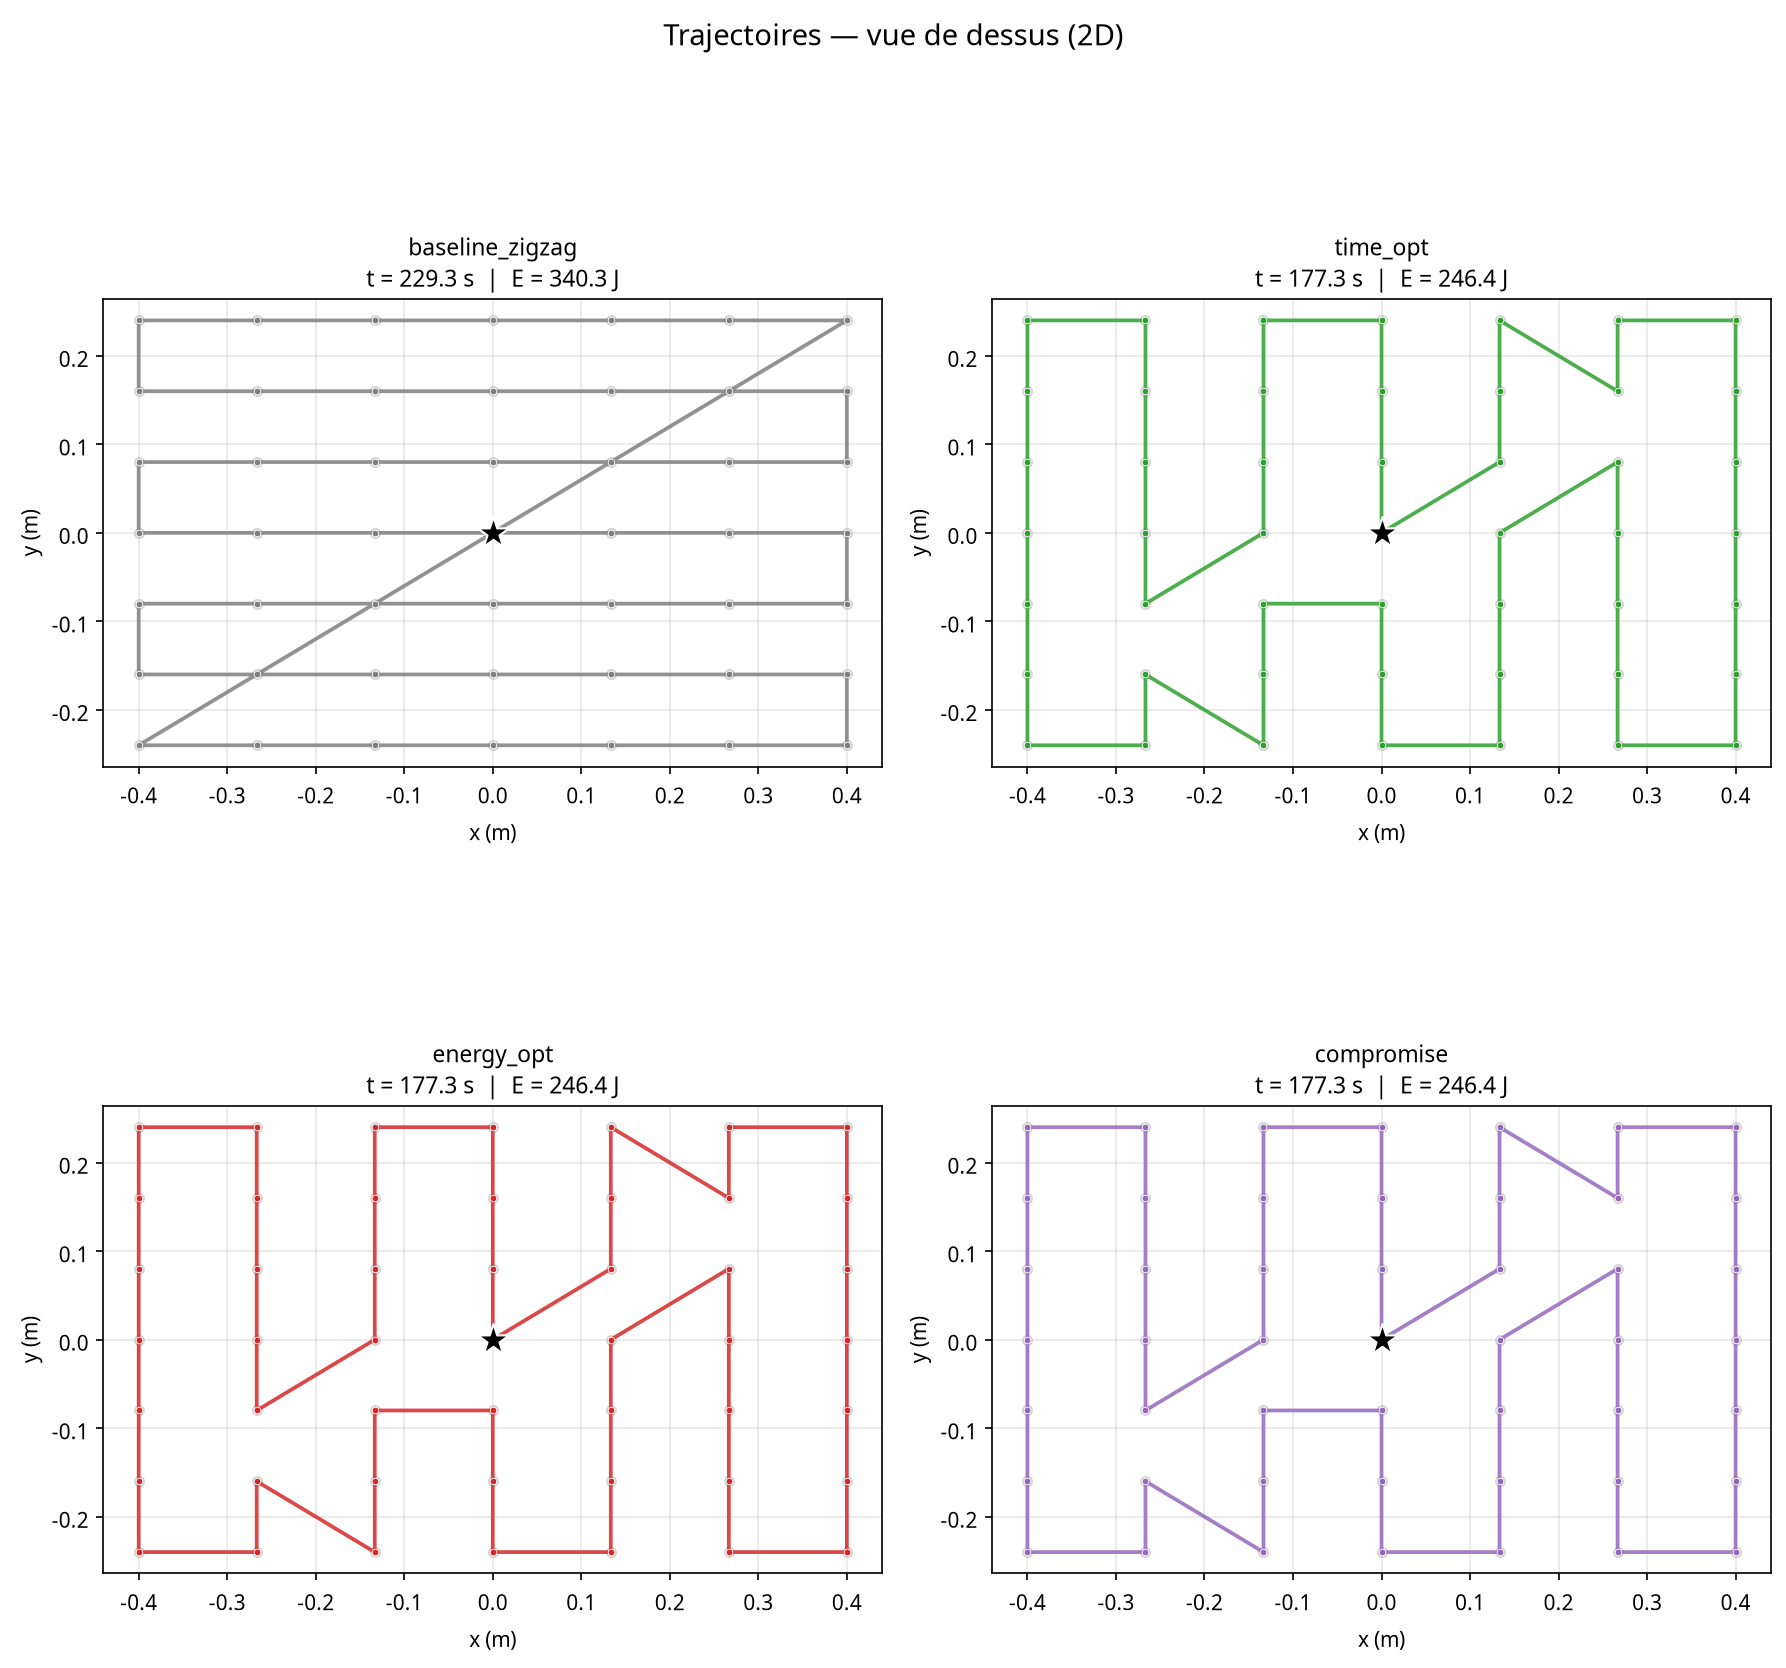
\includegraphics[width=\textwidth]{traj_sec_7x7.png}
\caption{Trajectoire en zone sécurisée pour grille $7\times7$}
\label{fig:traj_sec_7}
\end{figure}

La comparaison visuelle met en évidence la rupture entre la baseline en zigzag (gris) et les trajectoires optimisées. Le point clé est la superposition parfaite des trois courbes (vert, rouge, violet) : elles empruntent exactement le même chemin, confirmant visuellement que le front de Pareto se réduit à une solution unique (singleton) pour cette configuration. Contrairement au balayage systématique ligne par ligne, l'algorithme trace un parcours fluide qui évite les croisements et les retours inutiles, validant ainsi les gains de 22,7~\% en temps et de 27,6~\% en énergie observés sur la grille $7\times7$.

\clearpage
\begin{figure}[H]
\centering
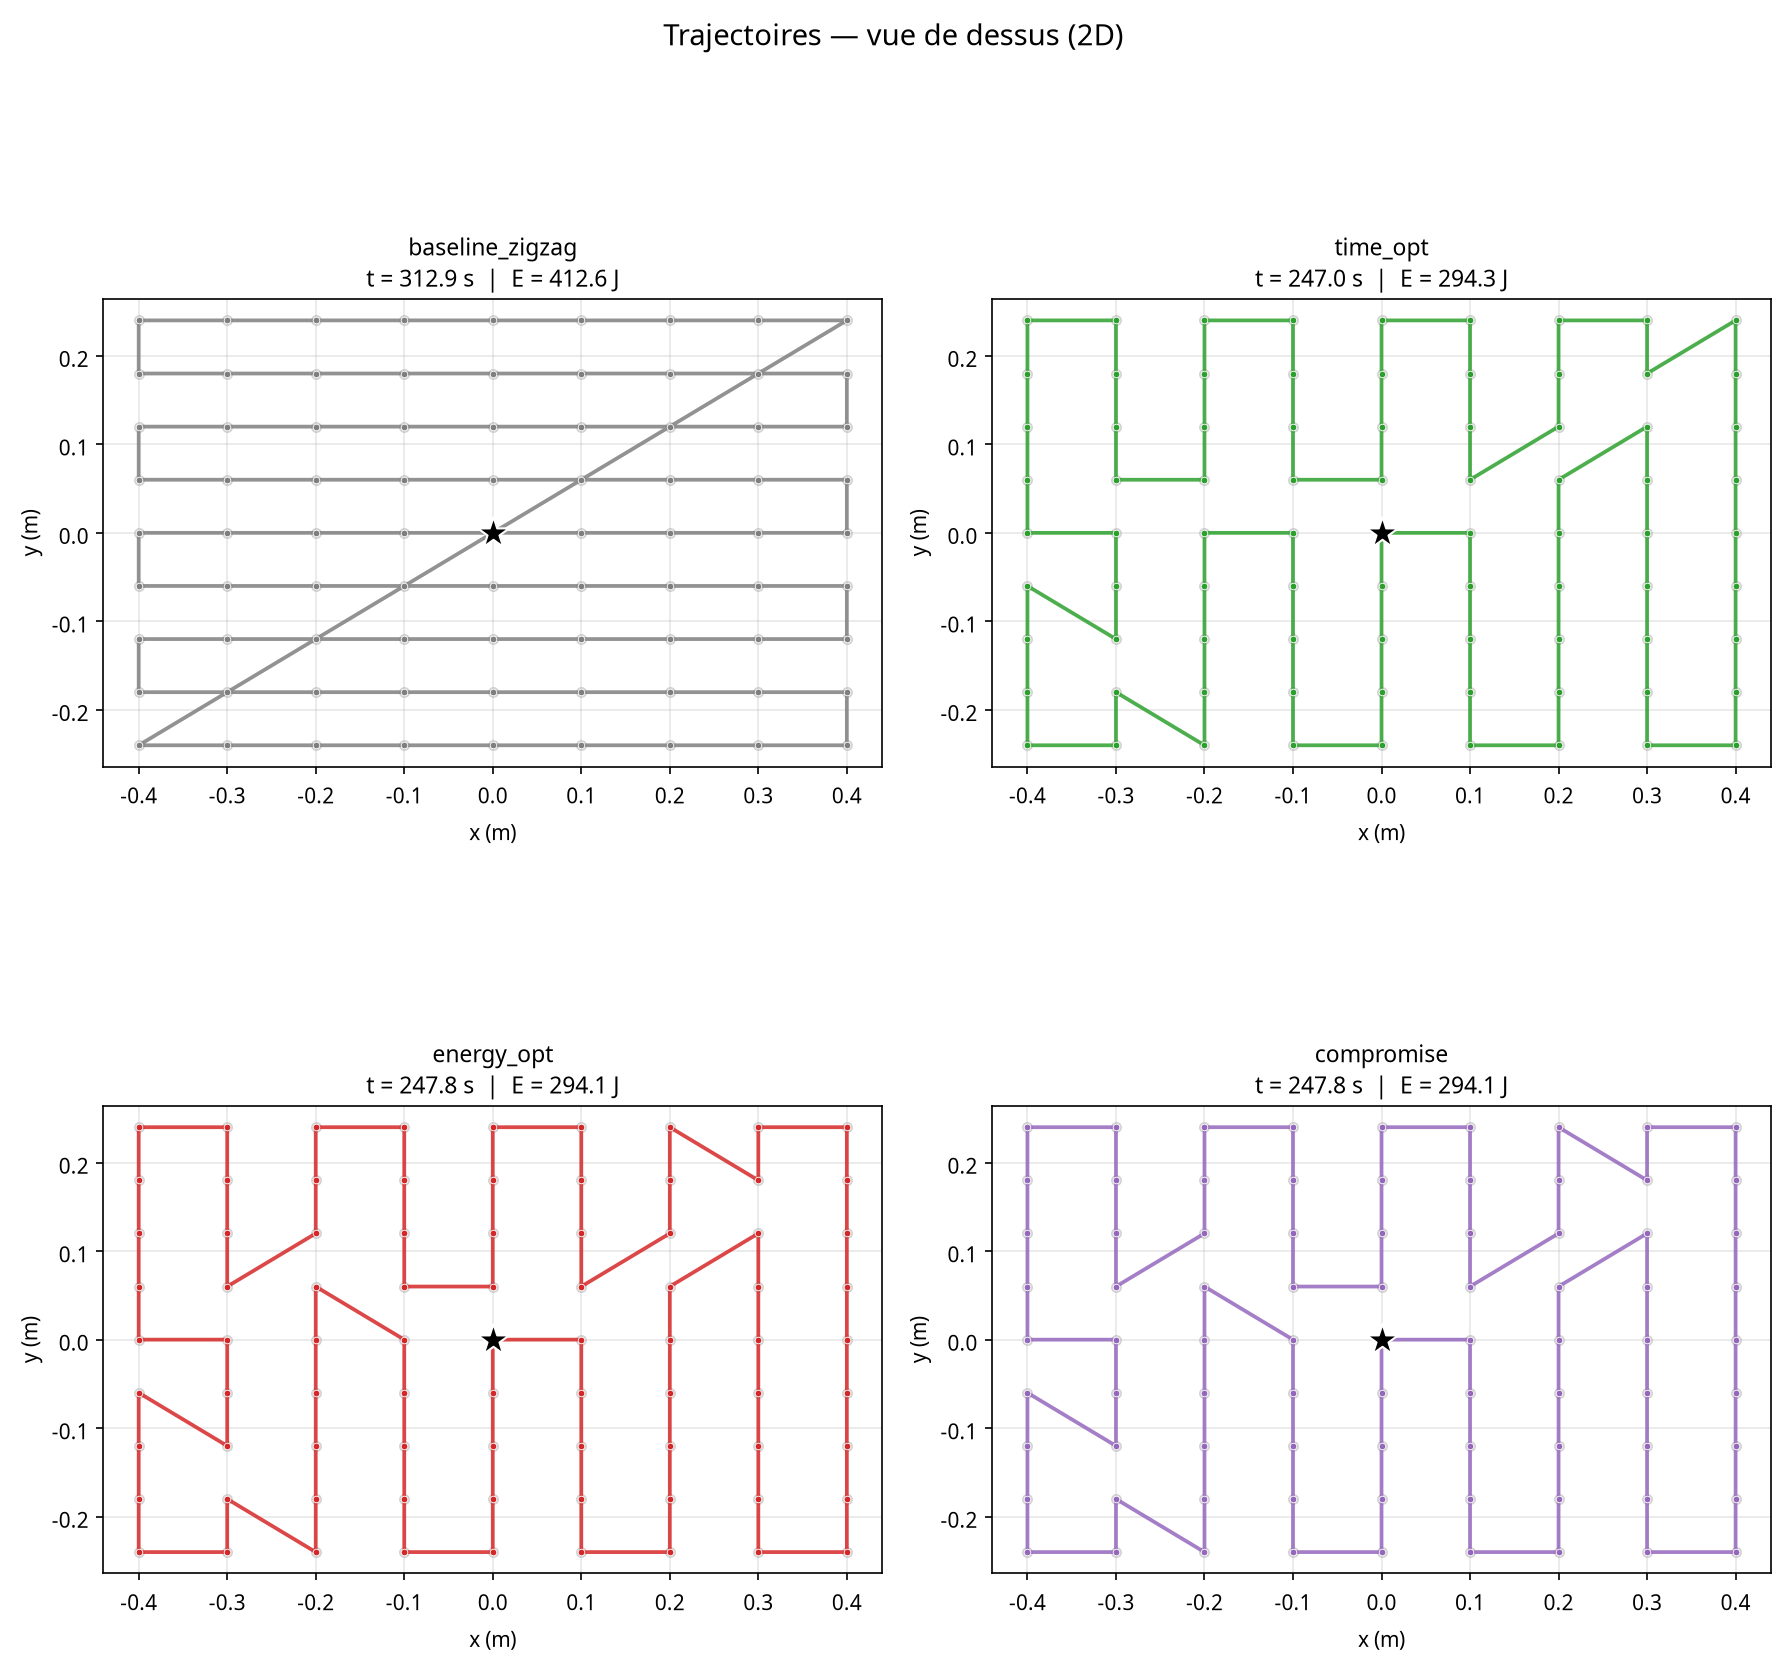
\includegraphics[width=\textwidth]{traj_sec_9x9.png}
\caption{Trajectoire en zone sécurisée pour grille $9\times9$}
\label{fig:traj_sec_9}
\end{figure}

\begin{figure}[H]
\centering
\begin{minipage}{0.48\textwidth}
\centering
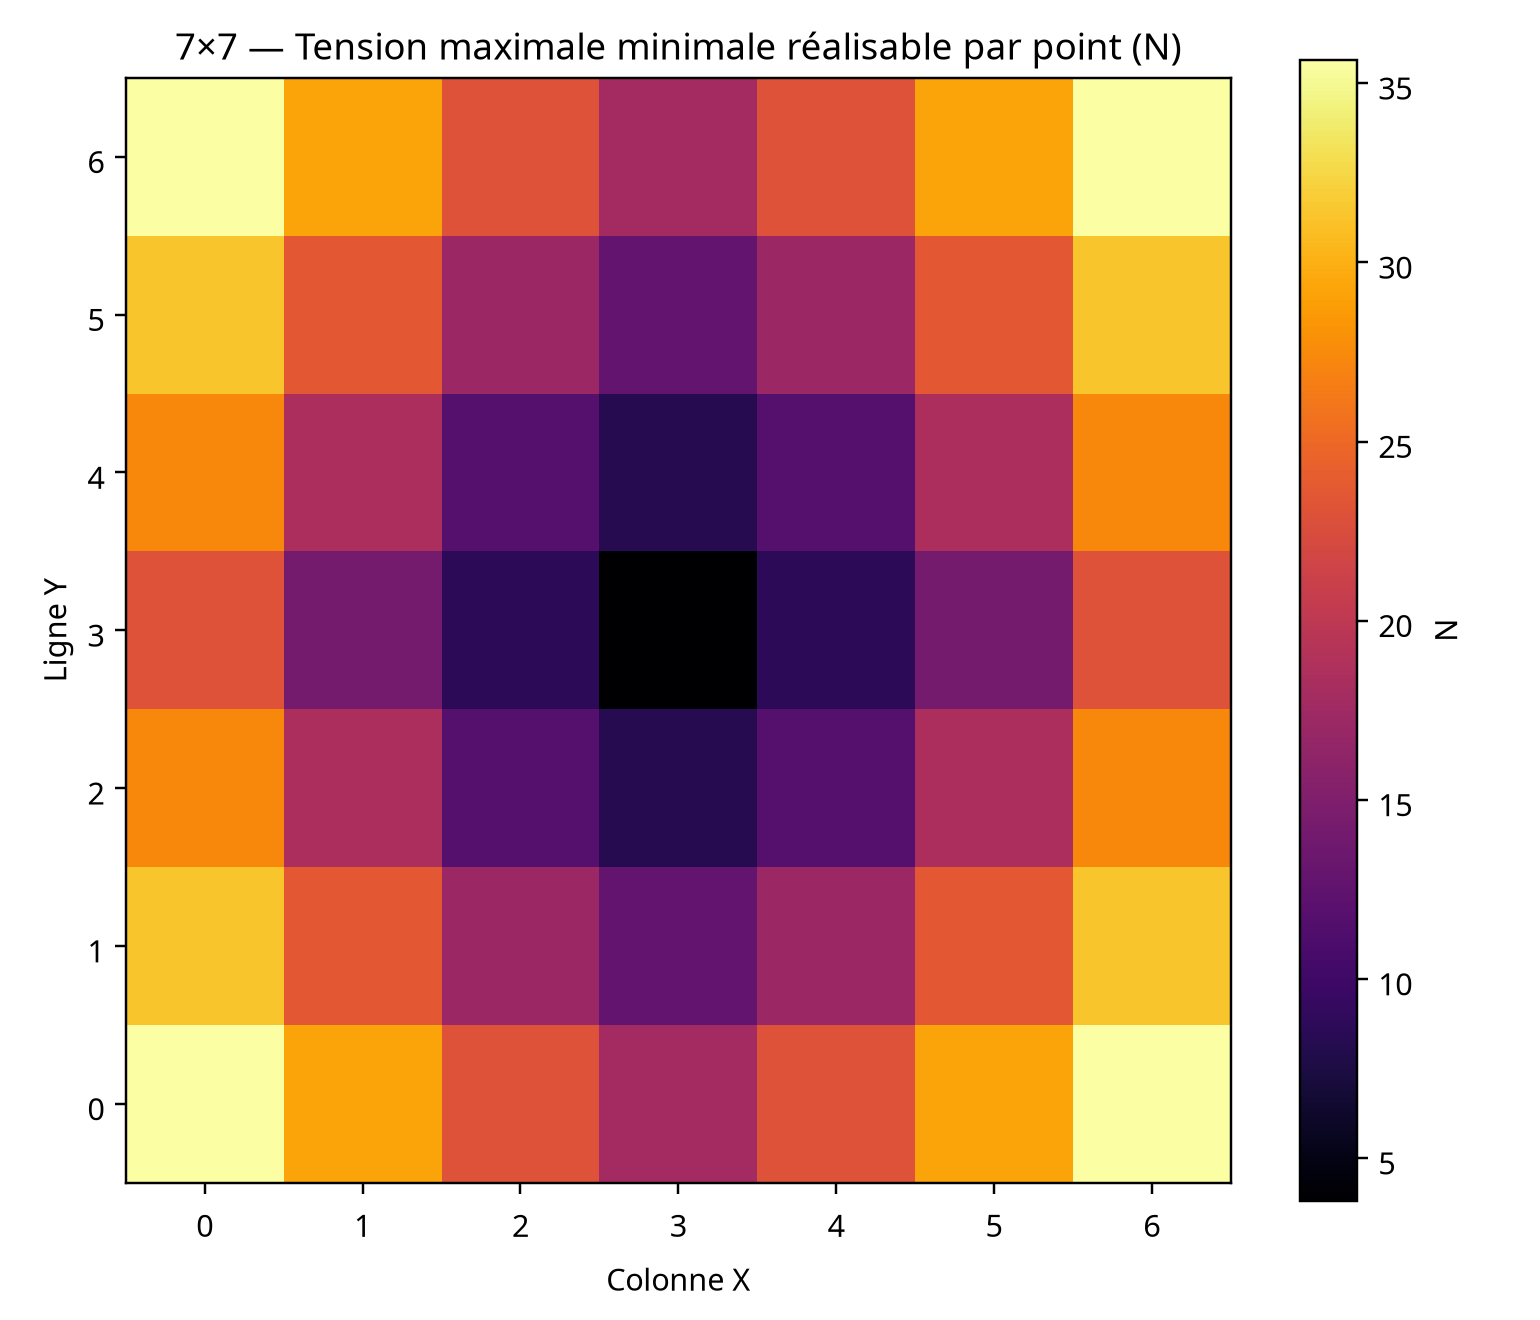
\includegraphics[width=\textwidth]{tens_maxmin.png}
\end{minipage}\hfill
\begin{minipage}{0.48\textwidth}
\centering
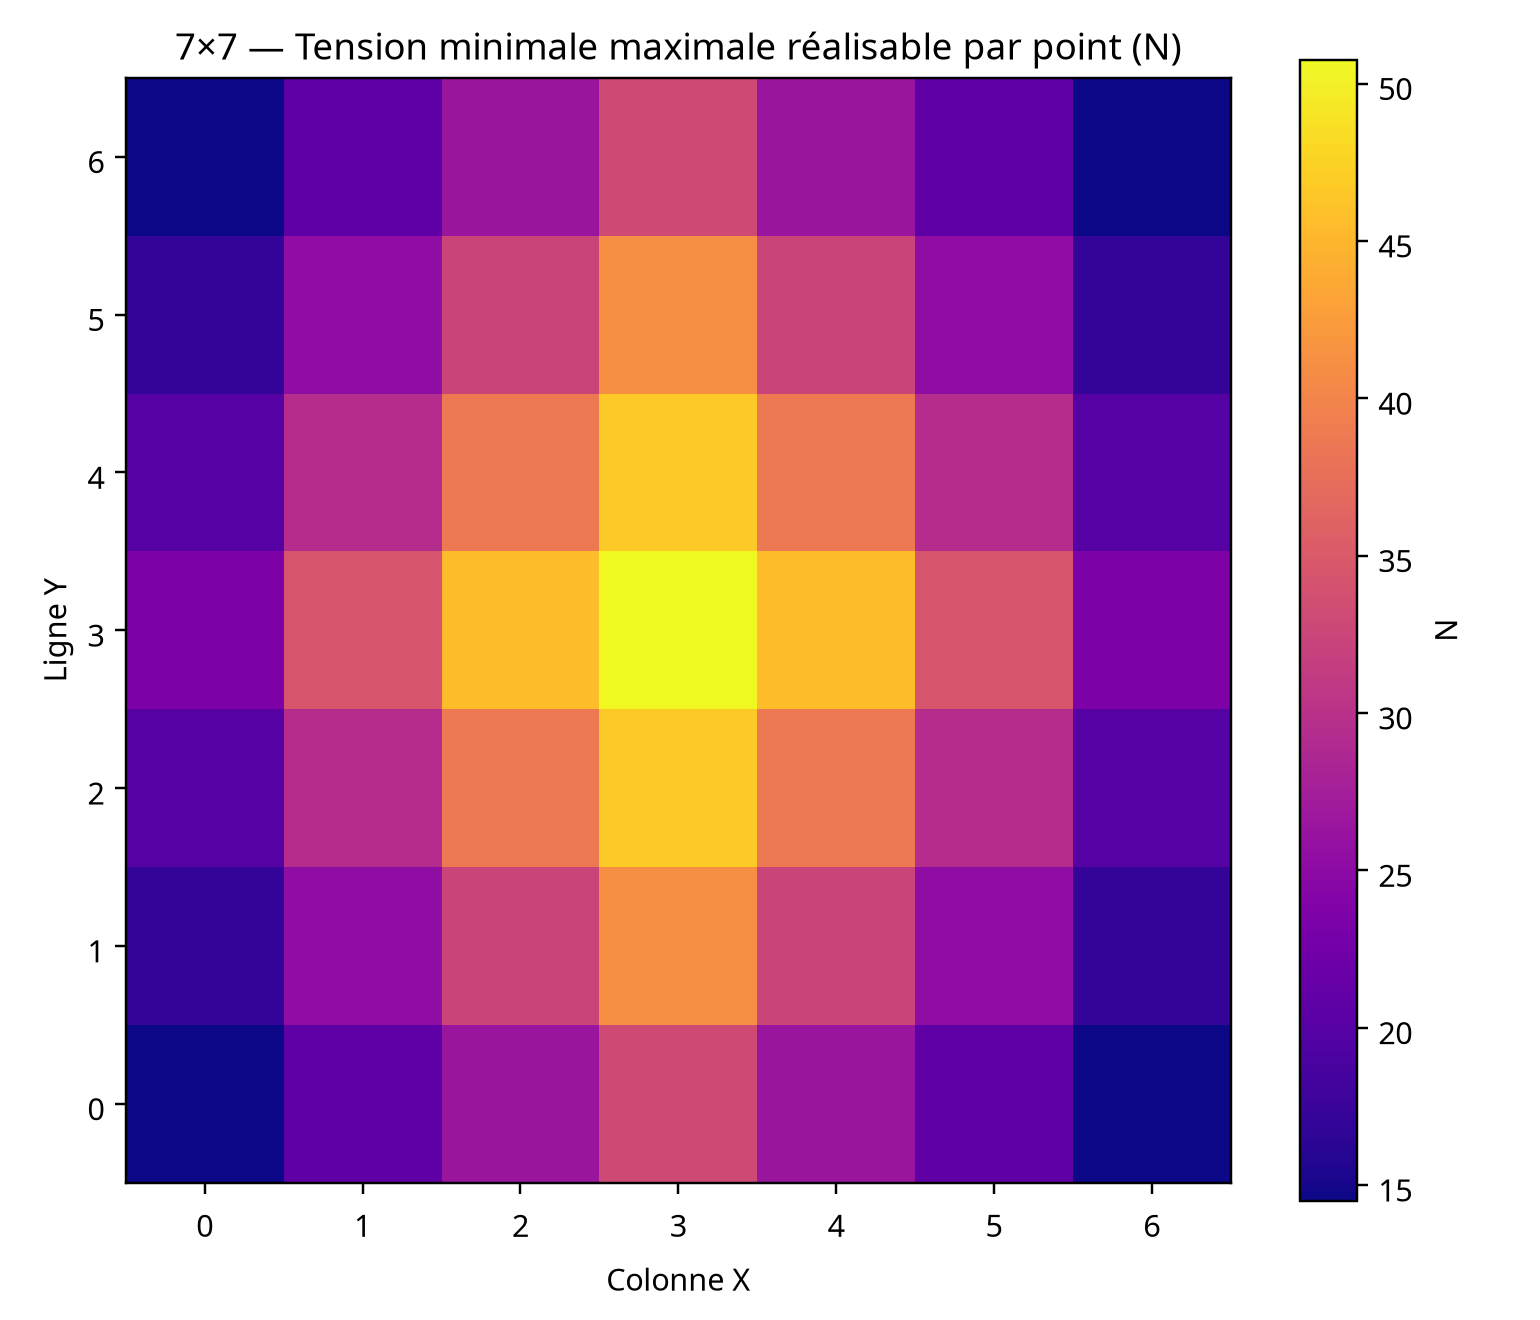
\includegraphics[width=\textwidth]{tens_minmax.png}
\end{minipage}
\caption{Tension des câbles par point pour grille $7\times7$}
\label{fig:tension}
\end{figure}

La répartition spatiale des tensions met en évidence un gradient marqué : minimale au centre (3,8~N), la tension requise augmente fortement vers les bords de la grille (jusqu'à 35,7~N) en raison de l'éloignement des ancrages. Cette élévation valide la robustesse de l'approche, les tensions maximales restant largement inférieures à la limite de sécurité de 58~N.


Sur la zone sécurisée $7\times7$, la tension maximale minimale varie de 3,8~N au centre à 35,7~N au bord (marge de 22,3~N sous la limite de 58~N).

\subsection{Effet de la couverture de la zone de travail}

Sur la grille $7\times7$ étendue : temps minimal 191,83~s / 315,61~J (gain 22,9~\% / 25,5~\% face au zigzag). Sur la grille $9\times9$ étendue (77 points) : temps minimal 301,15~s, énergie 636,65~J (gains 2,0~\% / 2,7~\% face au plus proche voisin).

\begin{figure}[H]
\centering
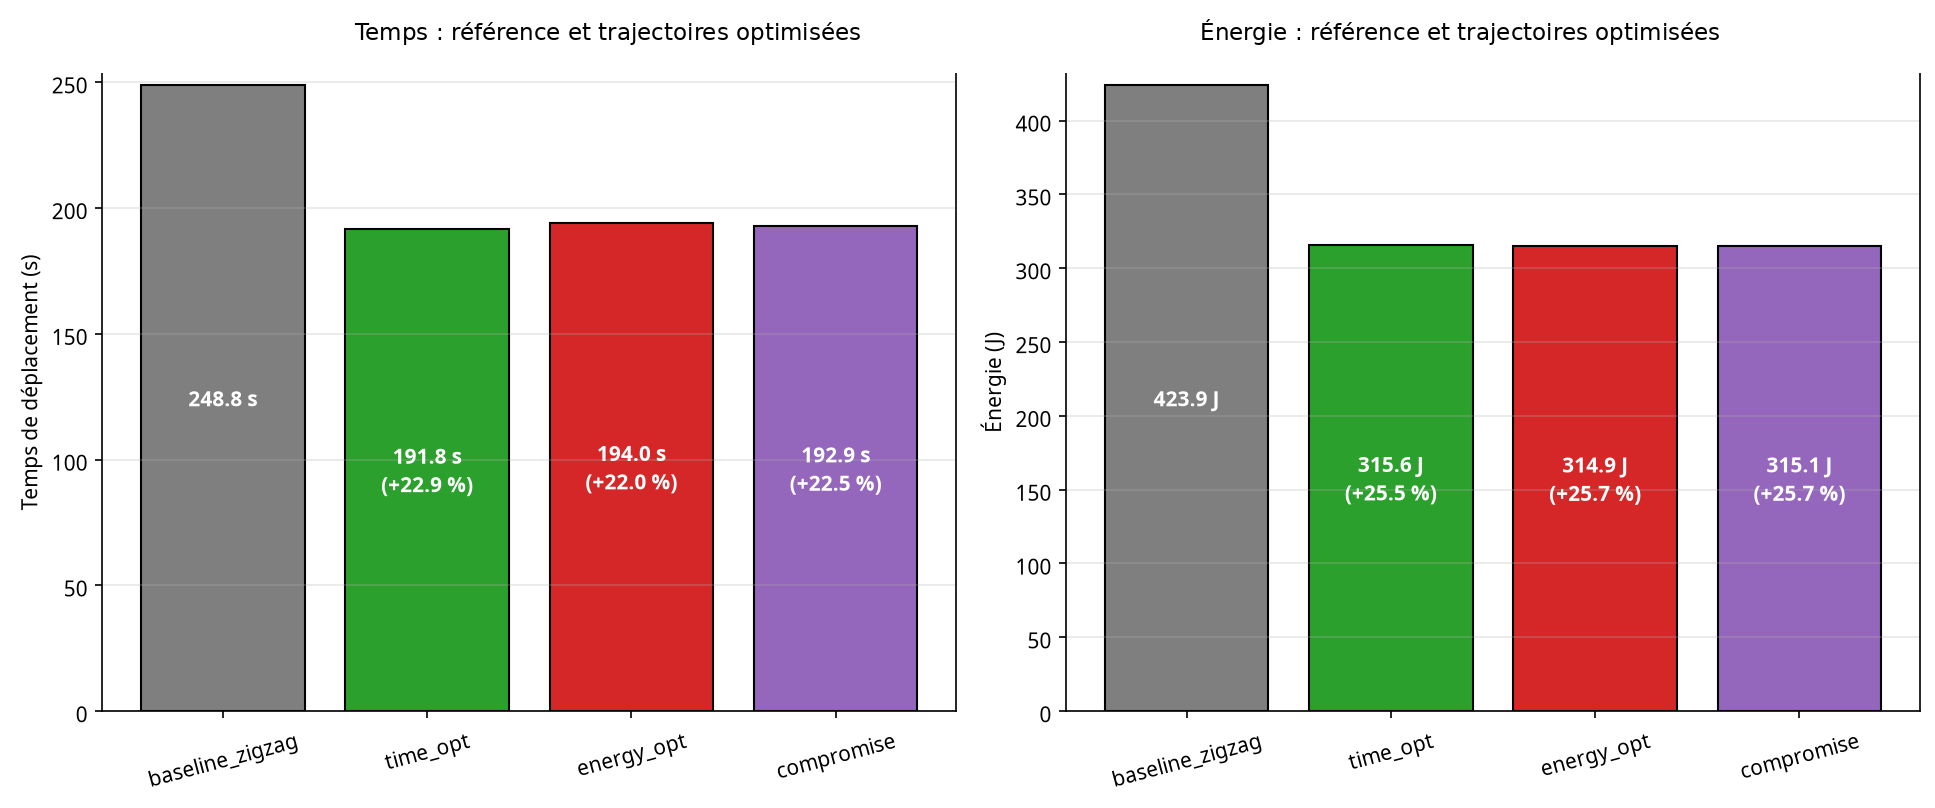
\includegraphics[width=0.92\textwidth,height=0.34\textheight,keepaspectratio]{comp_ext_7x7.png}\\[0.3em]
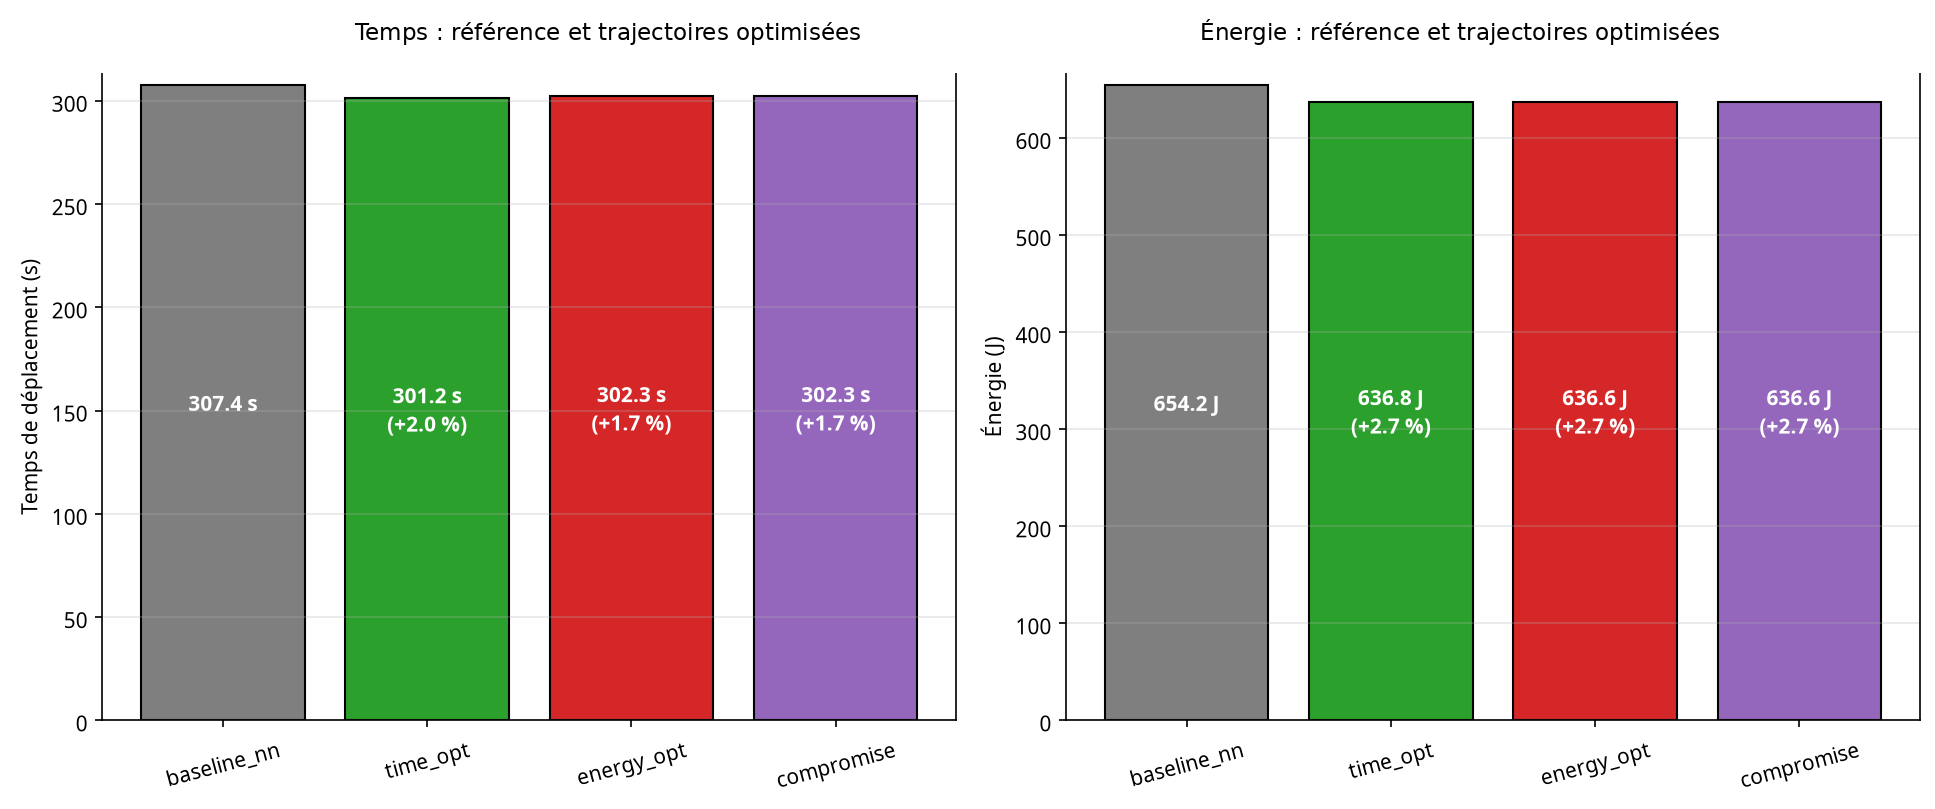
\includegraphics[width=0.92\textwidth,height=0.34\textheight,keepaspectratio]{comp_ext_9x9.png}
\caption{Temps et énergie, zone étendue}
\label{fig:comp_ext}
\end{figure}

\begin{figure}[H]
\centering
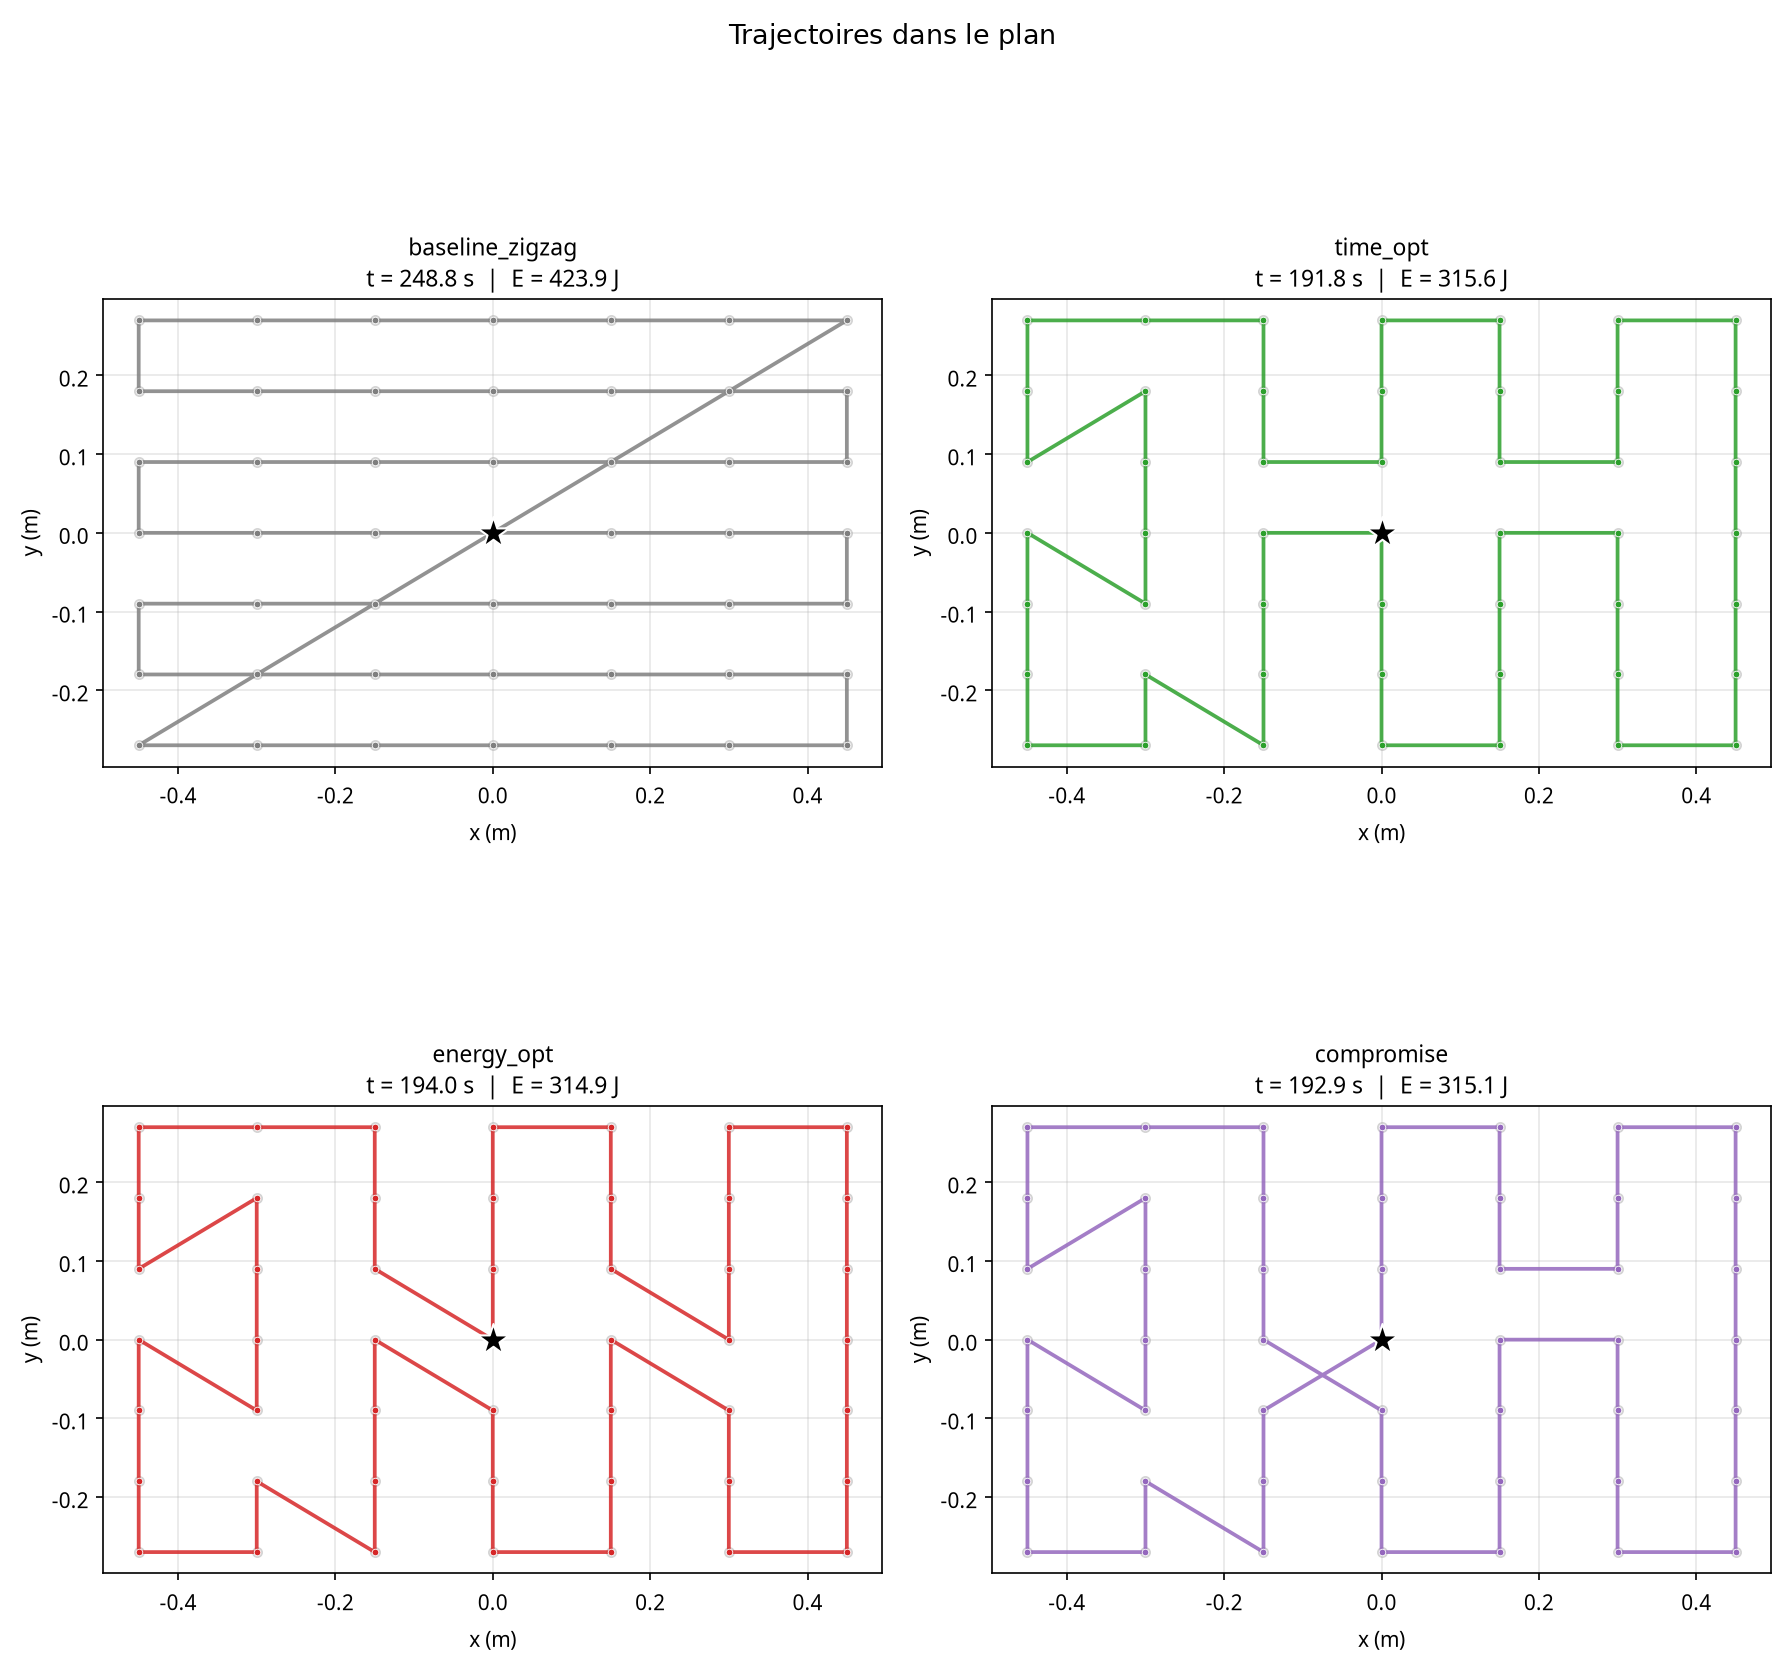
\includegraphics[width=\textwidth,height=0.78\textheight,keepaspectratio]{traj_ext_7x7.png}
\caption{Tracé 2D des trajectoires, zone étendue — grille $7\times7$}
\label{fig:traj_ext_7}
\end{figure}

Le tracé comparatif met en évidence la supériorité des chemins optimisés (vert, rouge, violet) sur la baseline en zigzag (gris). On observe que l'algorithme évite les allers-retours systématiques et les croisements inutiles, réduisant ainsi la distance globale parcourue. Cette visualisation confirme le gain de 22,9~\% en temps : NSGA-II exploite efficacement l'espace élargi en trouvant un ordre de visite beaucoup plus fluide.


\begin{figure}[H]
\centering
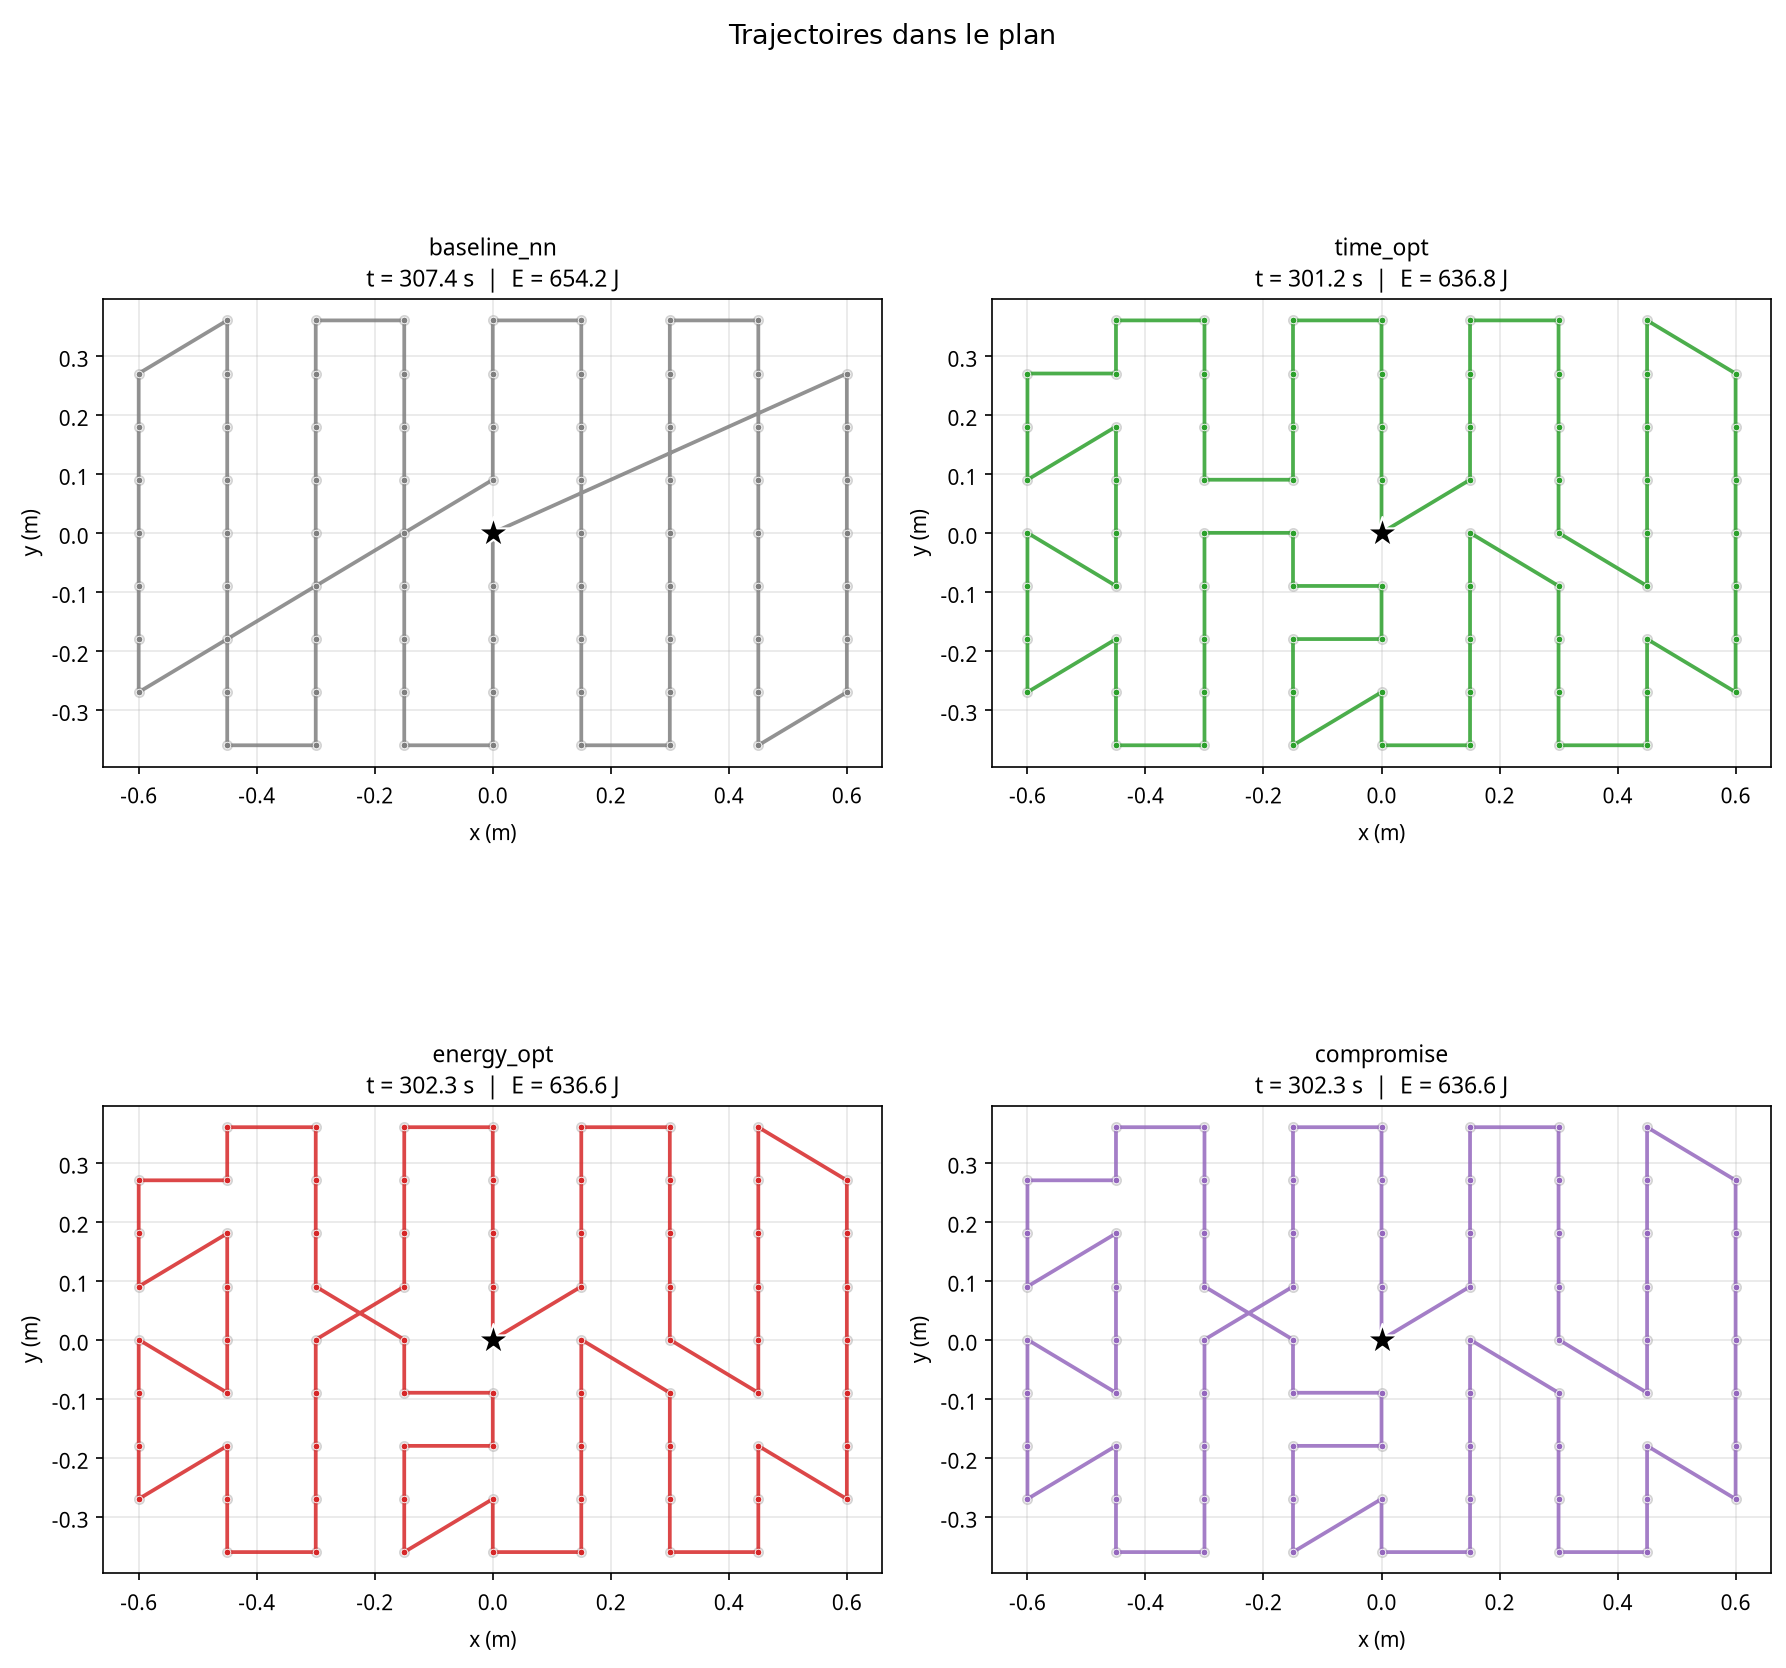
\includegraphics[width=\textwidth,height=0.78\textheight,keepaspectratio]{traj_ext_9x9.png}
\caption{Tracé 2D des trajectoires, zone étendue — grille $9\times9$}
\label{fig:traj_ext_9}
\end{figure}

La représentation de la grille $9\times9$ étendue (77 points, coins rejetés) révèle des trajectoires optimisées plus denses et complexes. Contrairement à la grille $7\times7$, les gains face à la baseline sont marginaux (2,0~\% en temps), car le balayage colonne par colonne est déjà naturellement proche de l'optimum pour un maillage aussi fin. L'optimisation démontre néanmoins sa capacité à gérer des espaces non convexes en contournant les quatre coins infaisables tout en maintenant un trajet cohérent et sans croisement.


\begin{figure}[H]
\centering
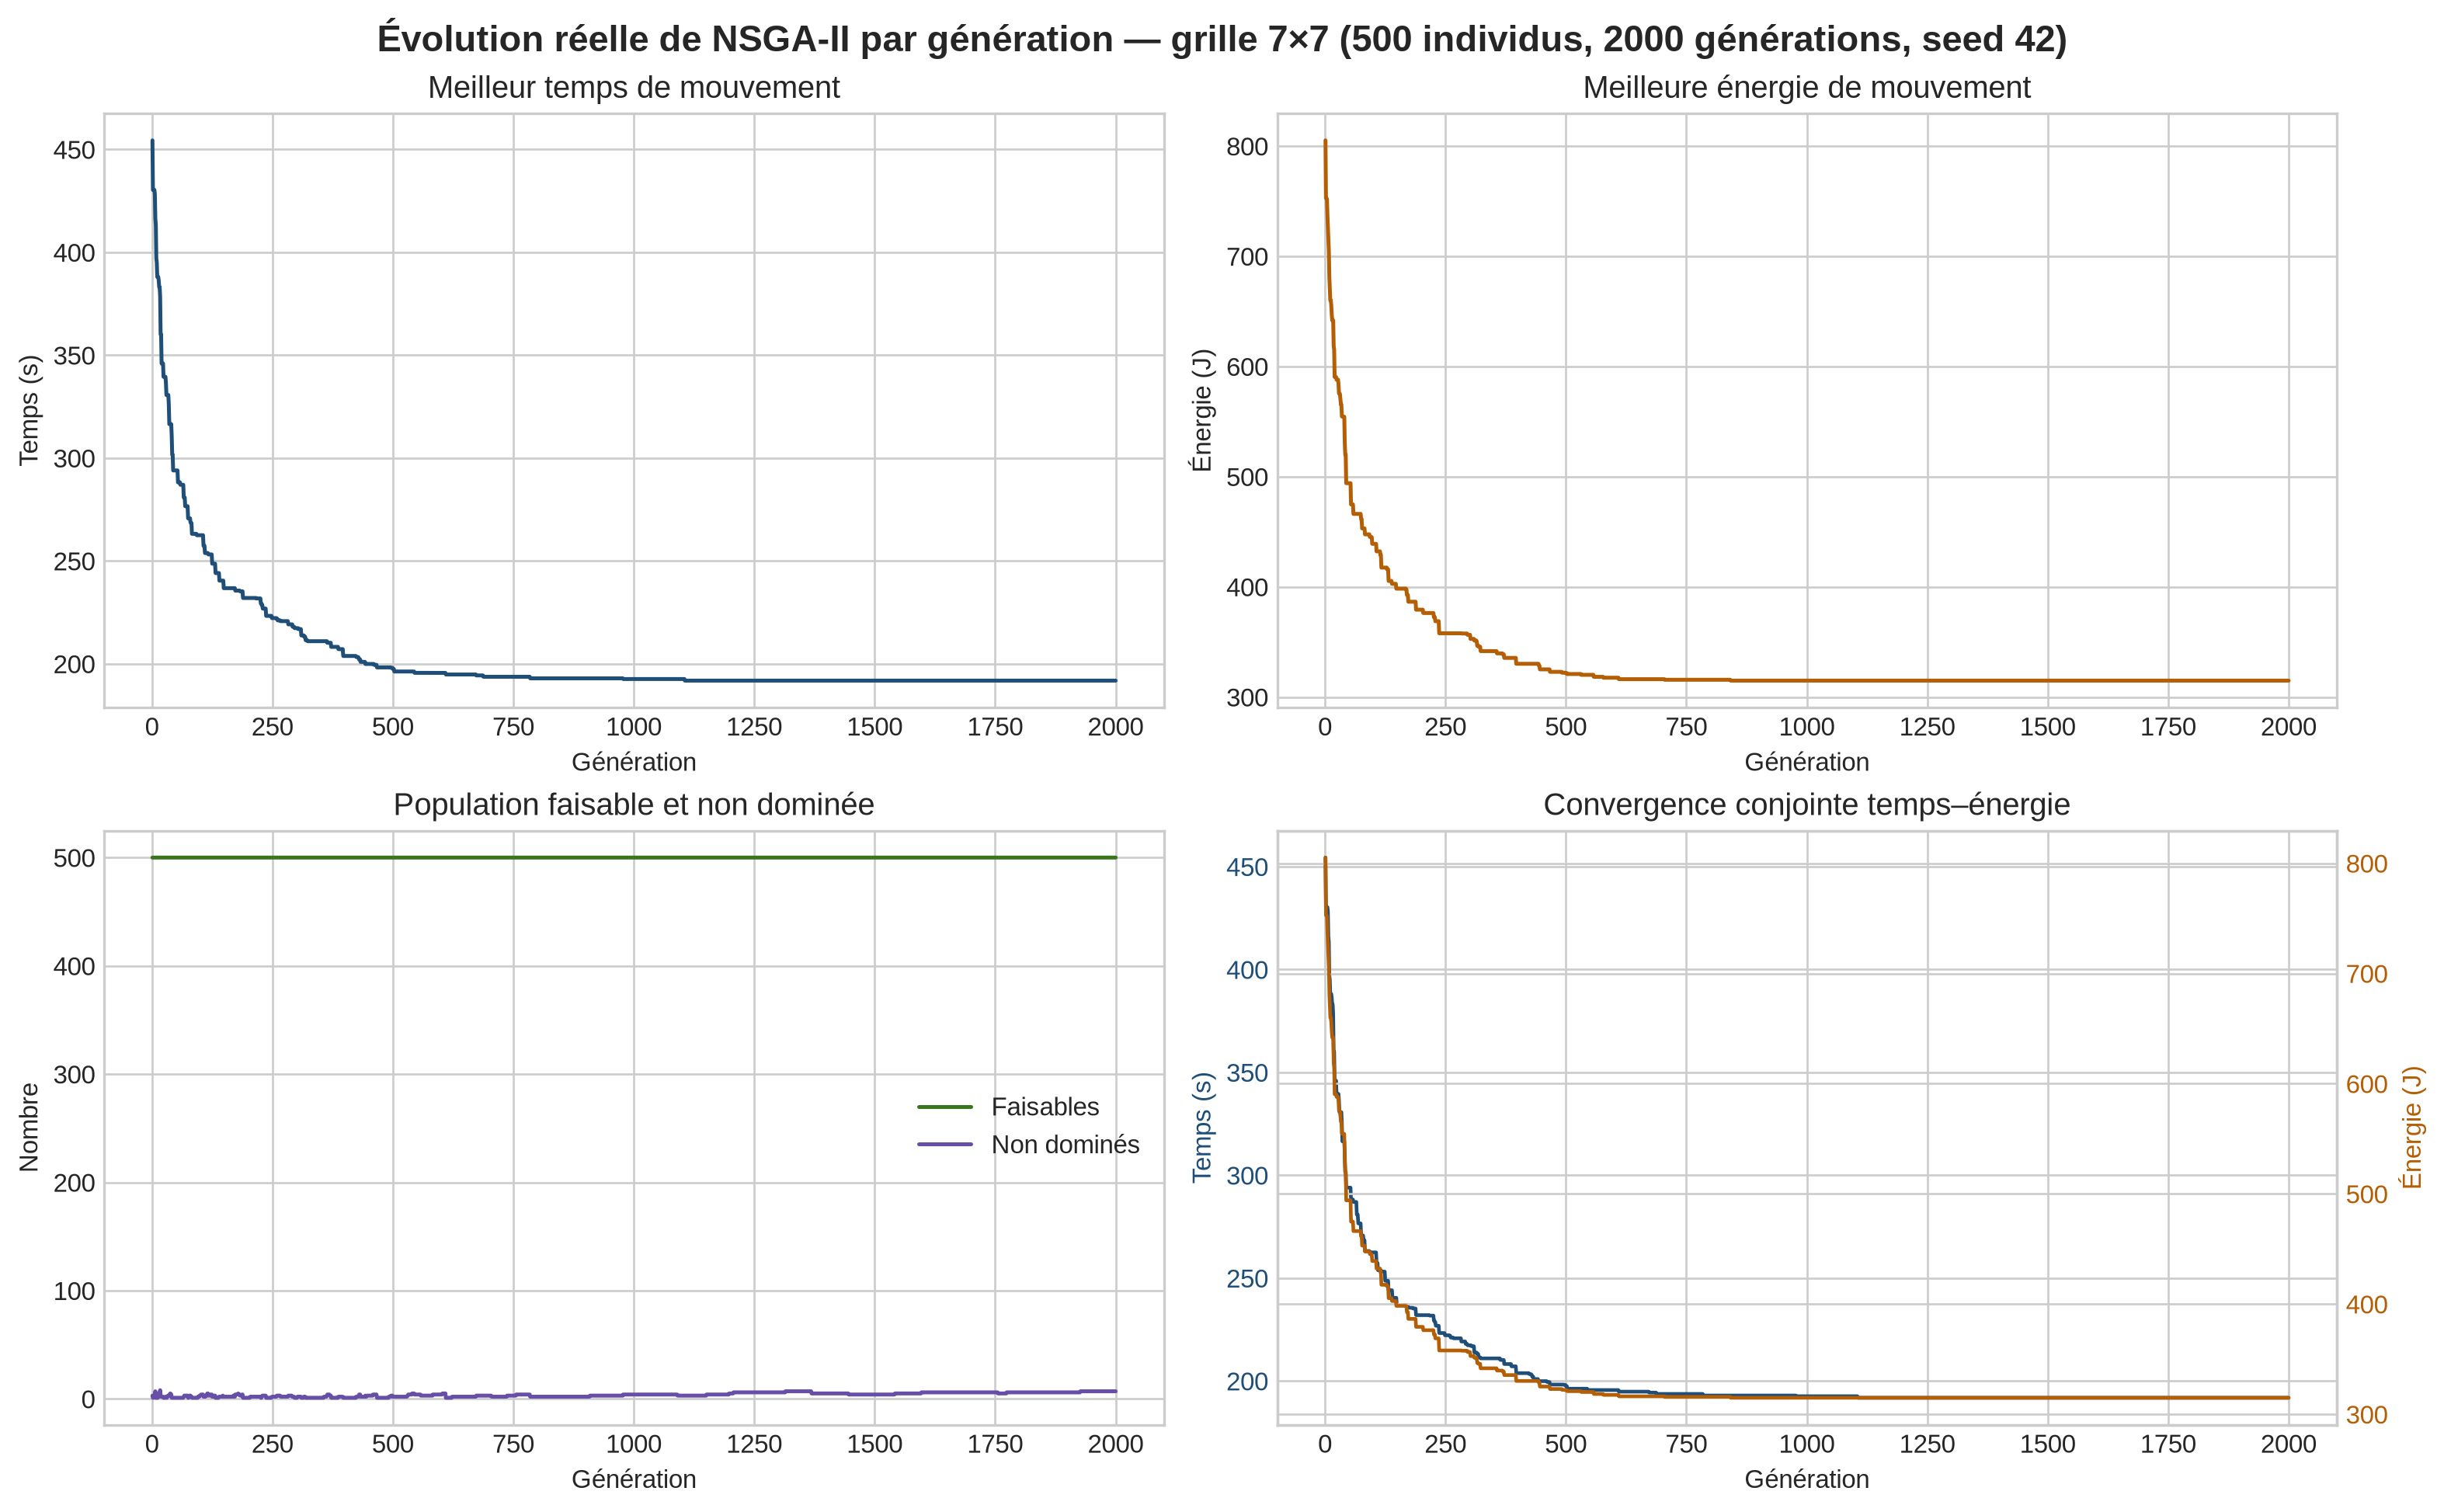
\includegraphics[width=0.95\textwidth,height=0.42\textheight,keepaspectratio]{conv_7x7.png}\\[0.35em]
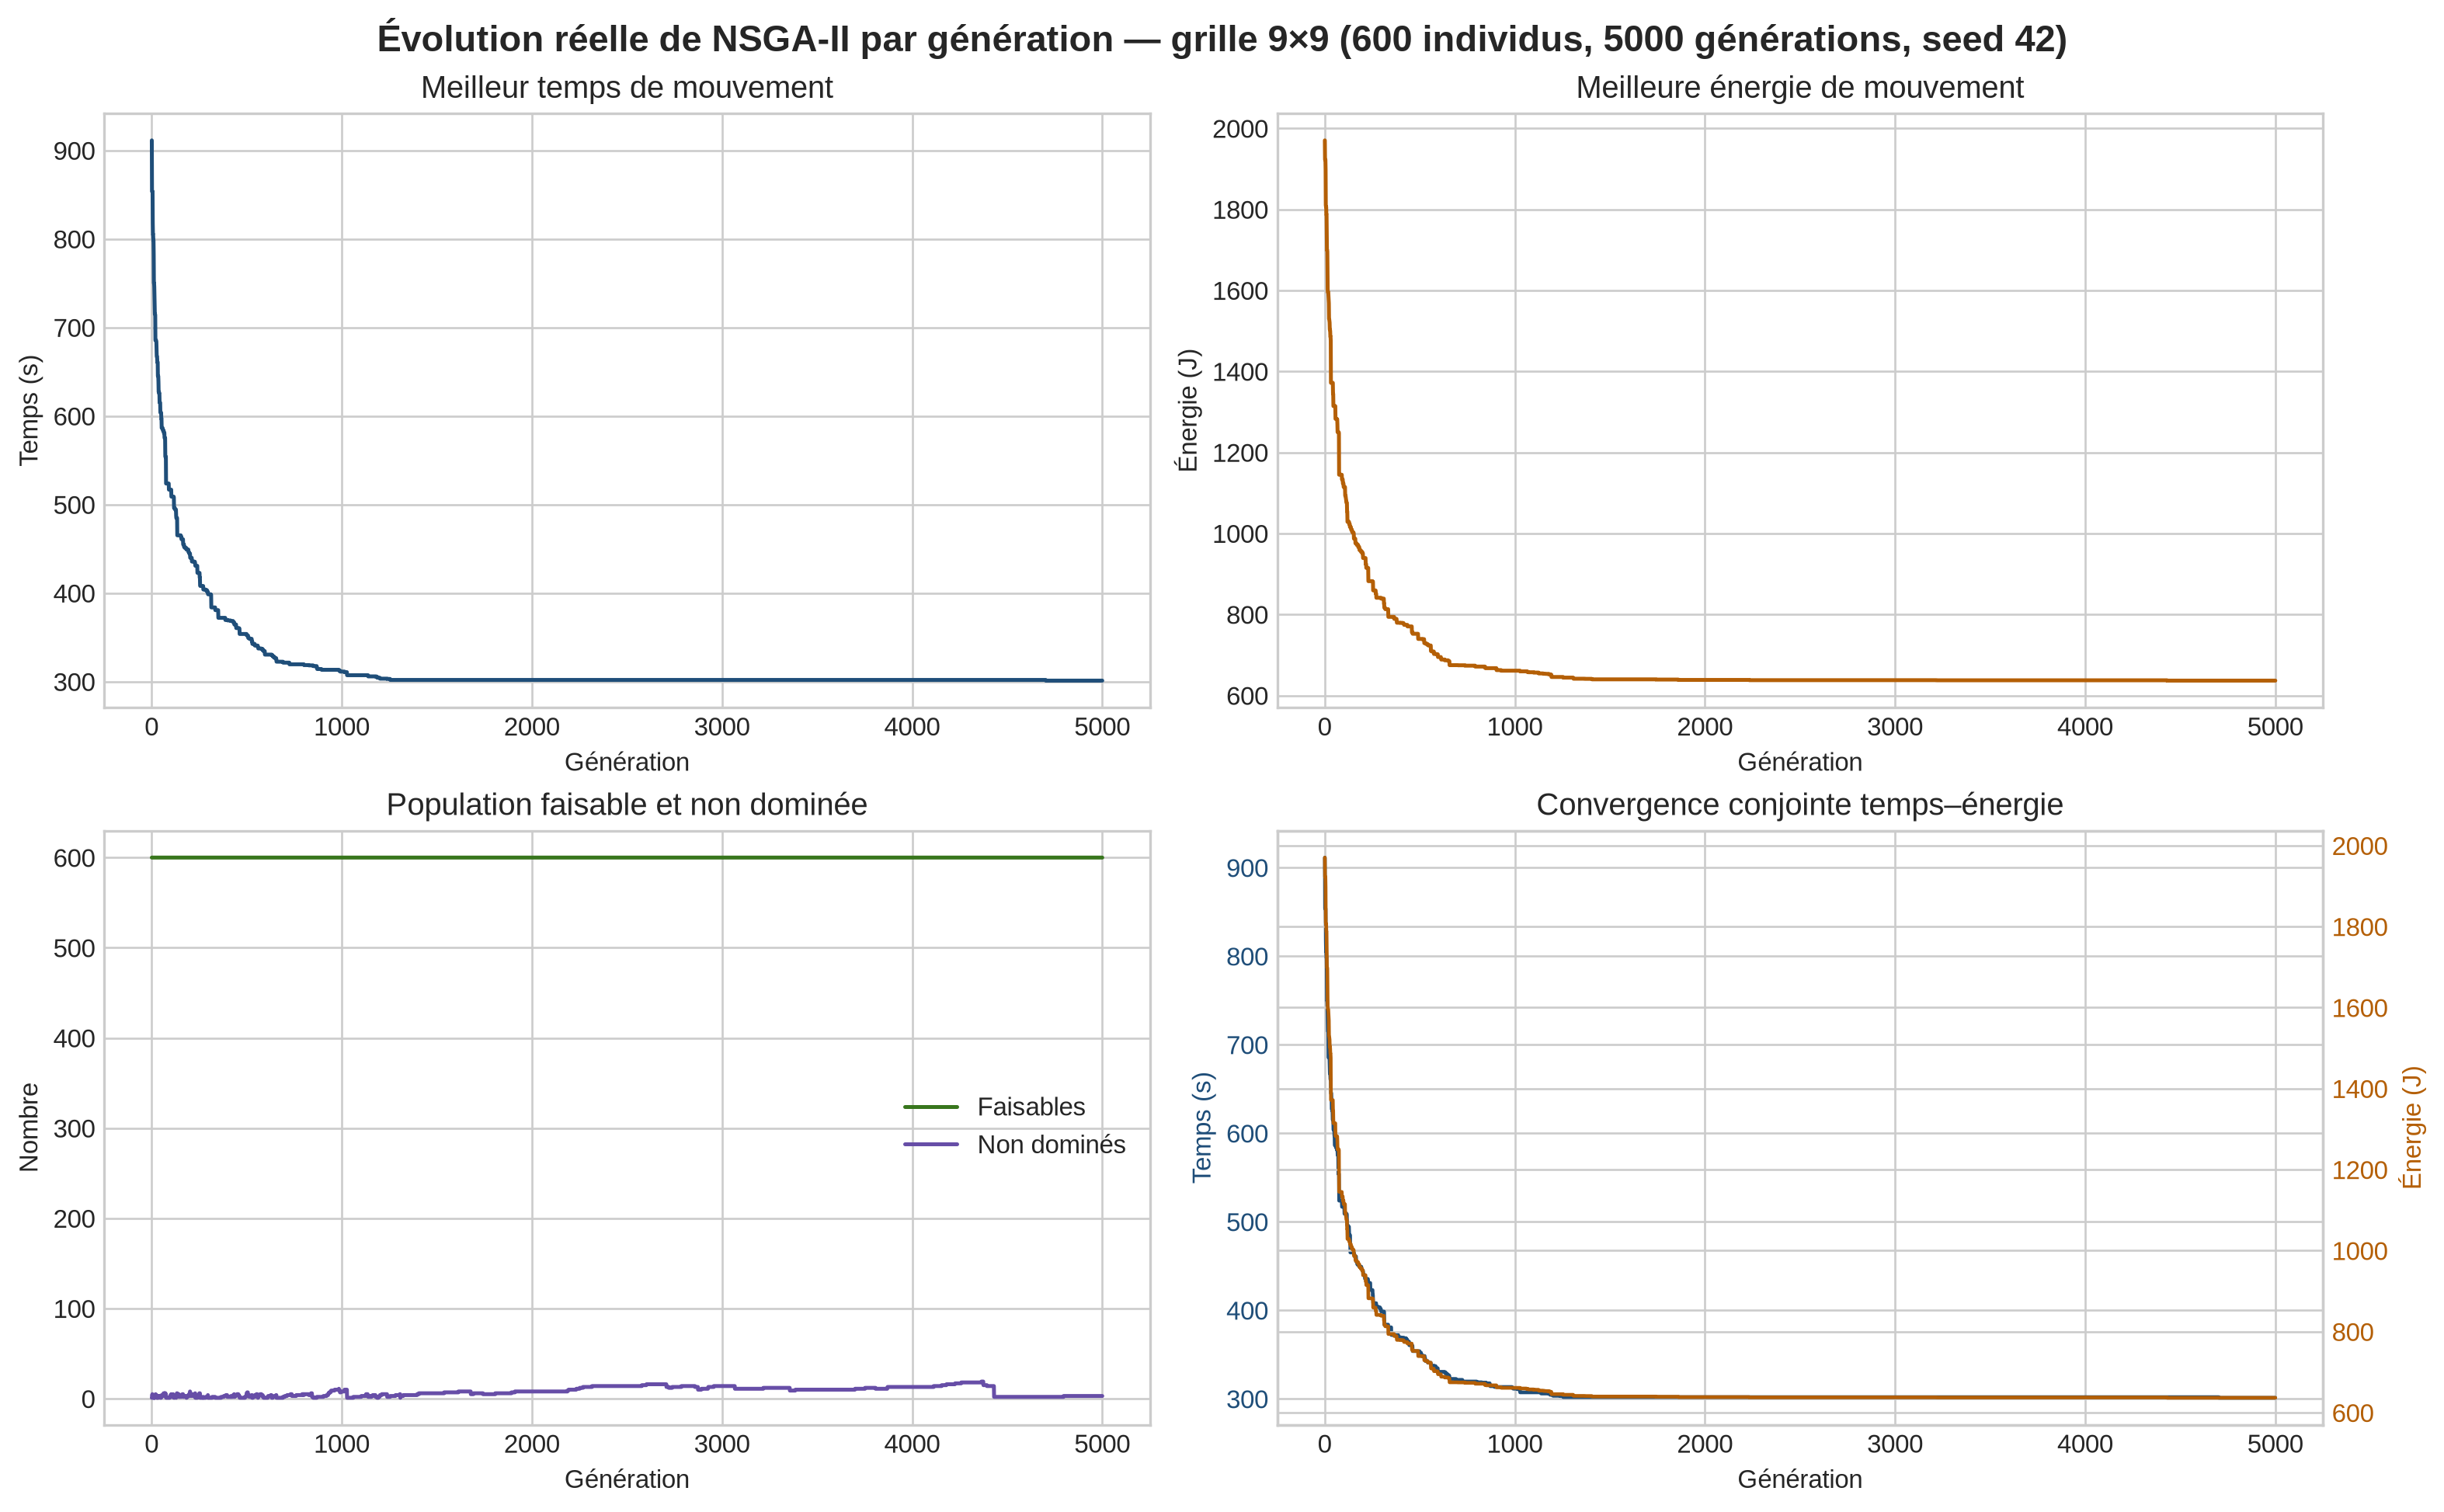
\includegraphics[width=0.95\textwidth,height=0.42\textheight,keepaspectratio]{conv_9x9.png}
\caption{Convergence de NSGA-II, zone étendue : (a) grille $7\times7$, (b) grille $9\times9$}
\label{fig:conv}
\end{figure}

L'évolution de l'algorithme au fil des générations est marquée par une chute rapide des coûts (temps et énergie), suivie d'un plateau asymptotique, tandis que la population maintient un taux de faisabilité de 100~\%. Cette dynamique confirme que les nombres de générations retenus (2000 et 5000) sont amplement suffisants pour atteindre l'optimum sans calculs superflus.


\begin{figure}[H]
\centering
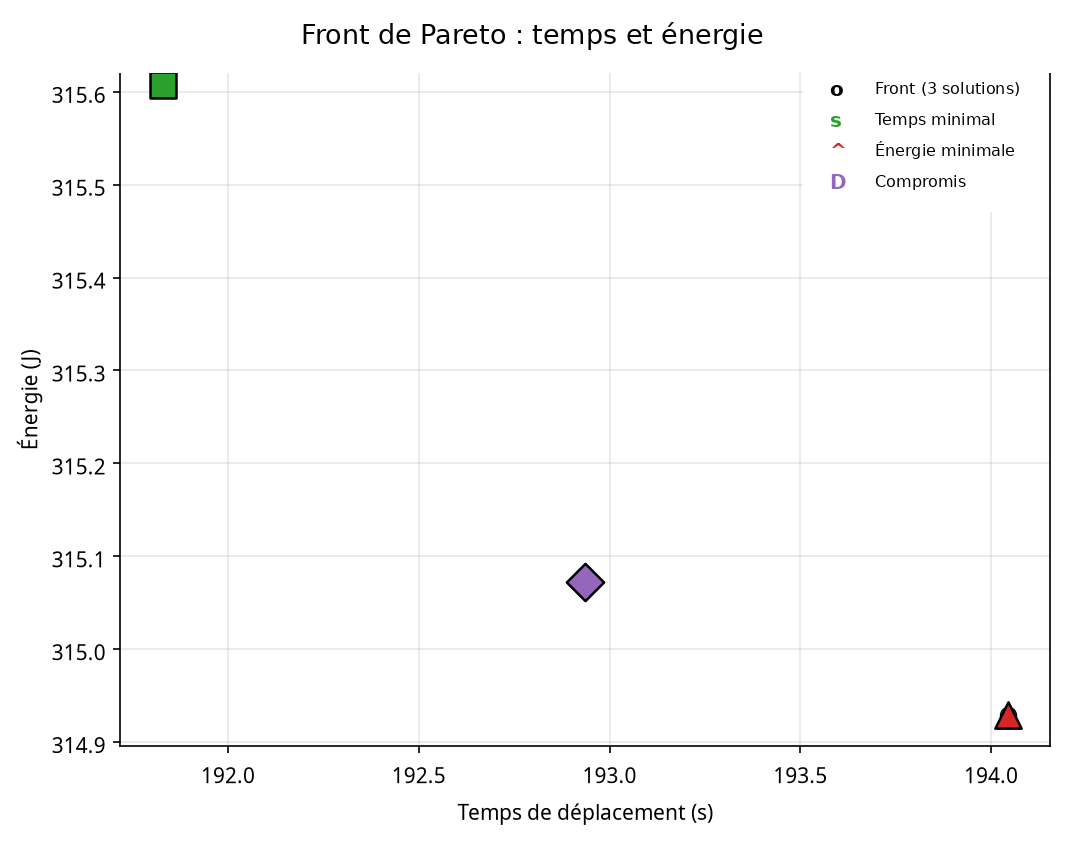
\includegraphics[width=0.92\textwidth,height=0.34\textheight,keepaspectratio]{pareto_7x7.png}\\[0.3em]
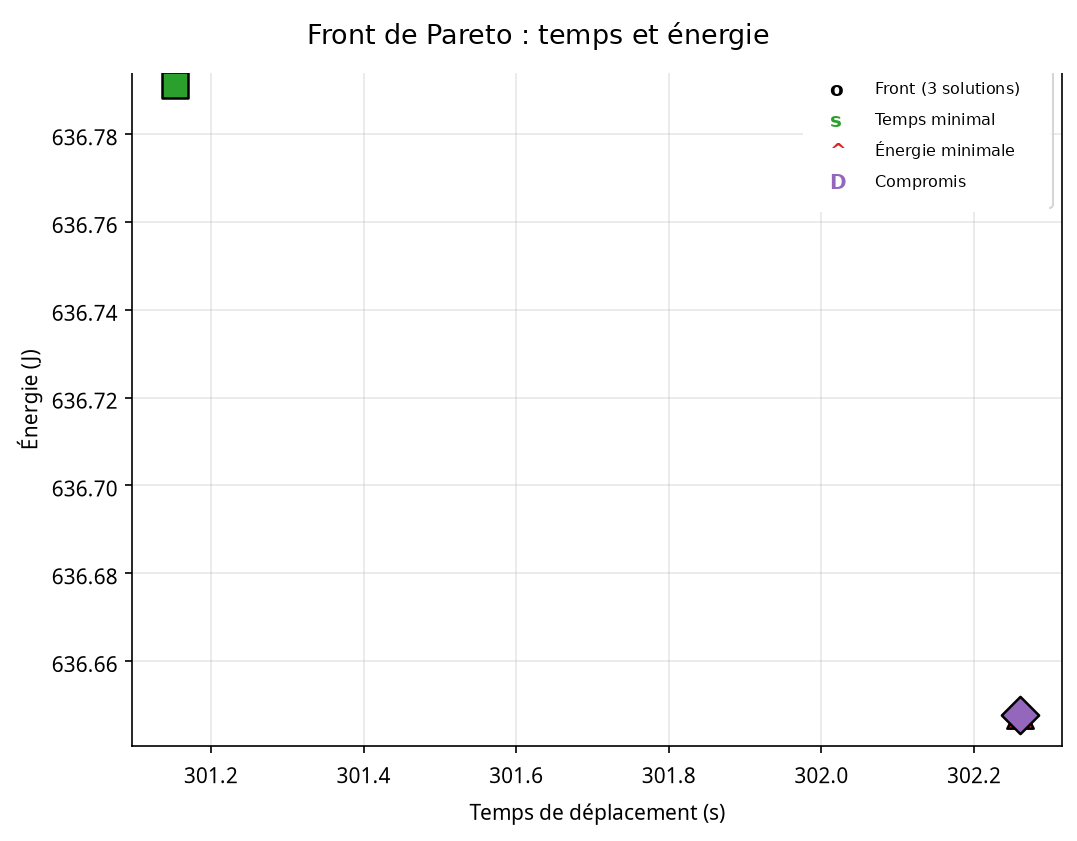
\includegraphics[width=0.92\textwidth,height=0.34\textheight,keepaspectratio]{pareto_9x9.png}
\caption{Fronts de Pareto temps--énergie, zone étendue}
\label{fig:pareto}
\end{figure}

L'analyse du front de Pareto révèle que les trois solutions optimales (temps minimal, énergie minimale et compromis) sont extrêmement proches les unes des autres. Cela démontre que, pour cette configuration, minimiser le temps ne dégrade pas significativement l'énergie, ce qui simplifie le choix de la trajectoire finale.


\begin{figure}[H]
\centering
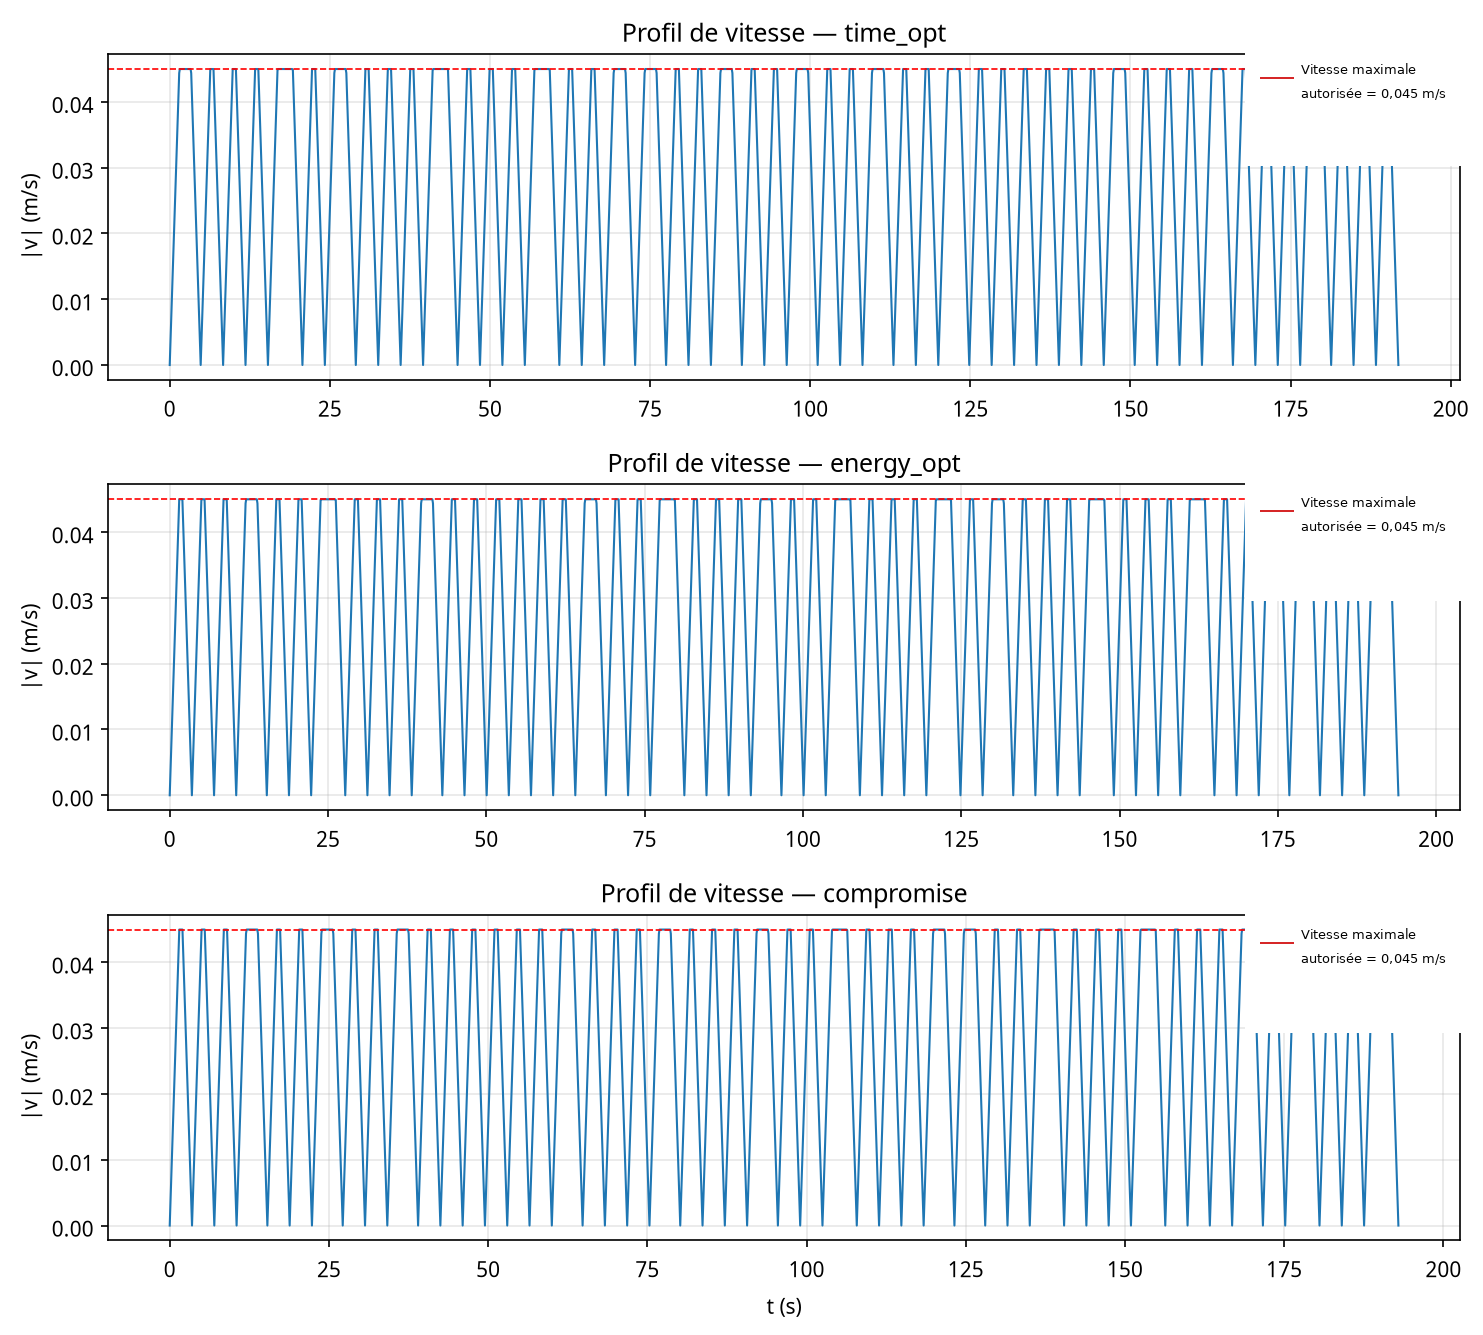
\includegraphics[width=0.92\textwidth,height=0.34\textheight,keepaspectratio]{prof_7x7.png}\\[0.3em]
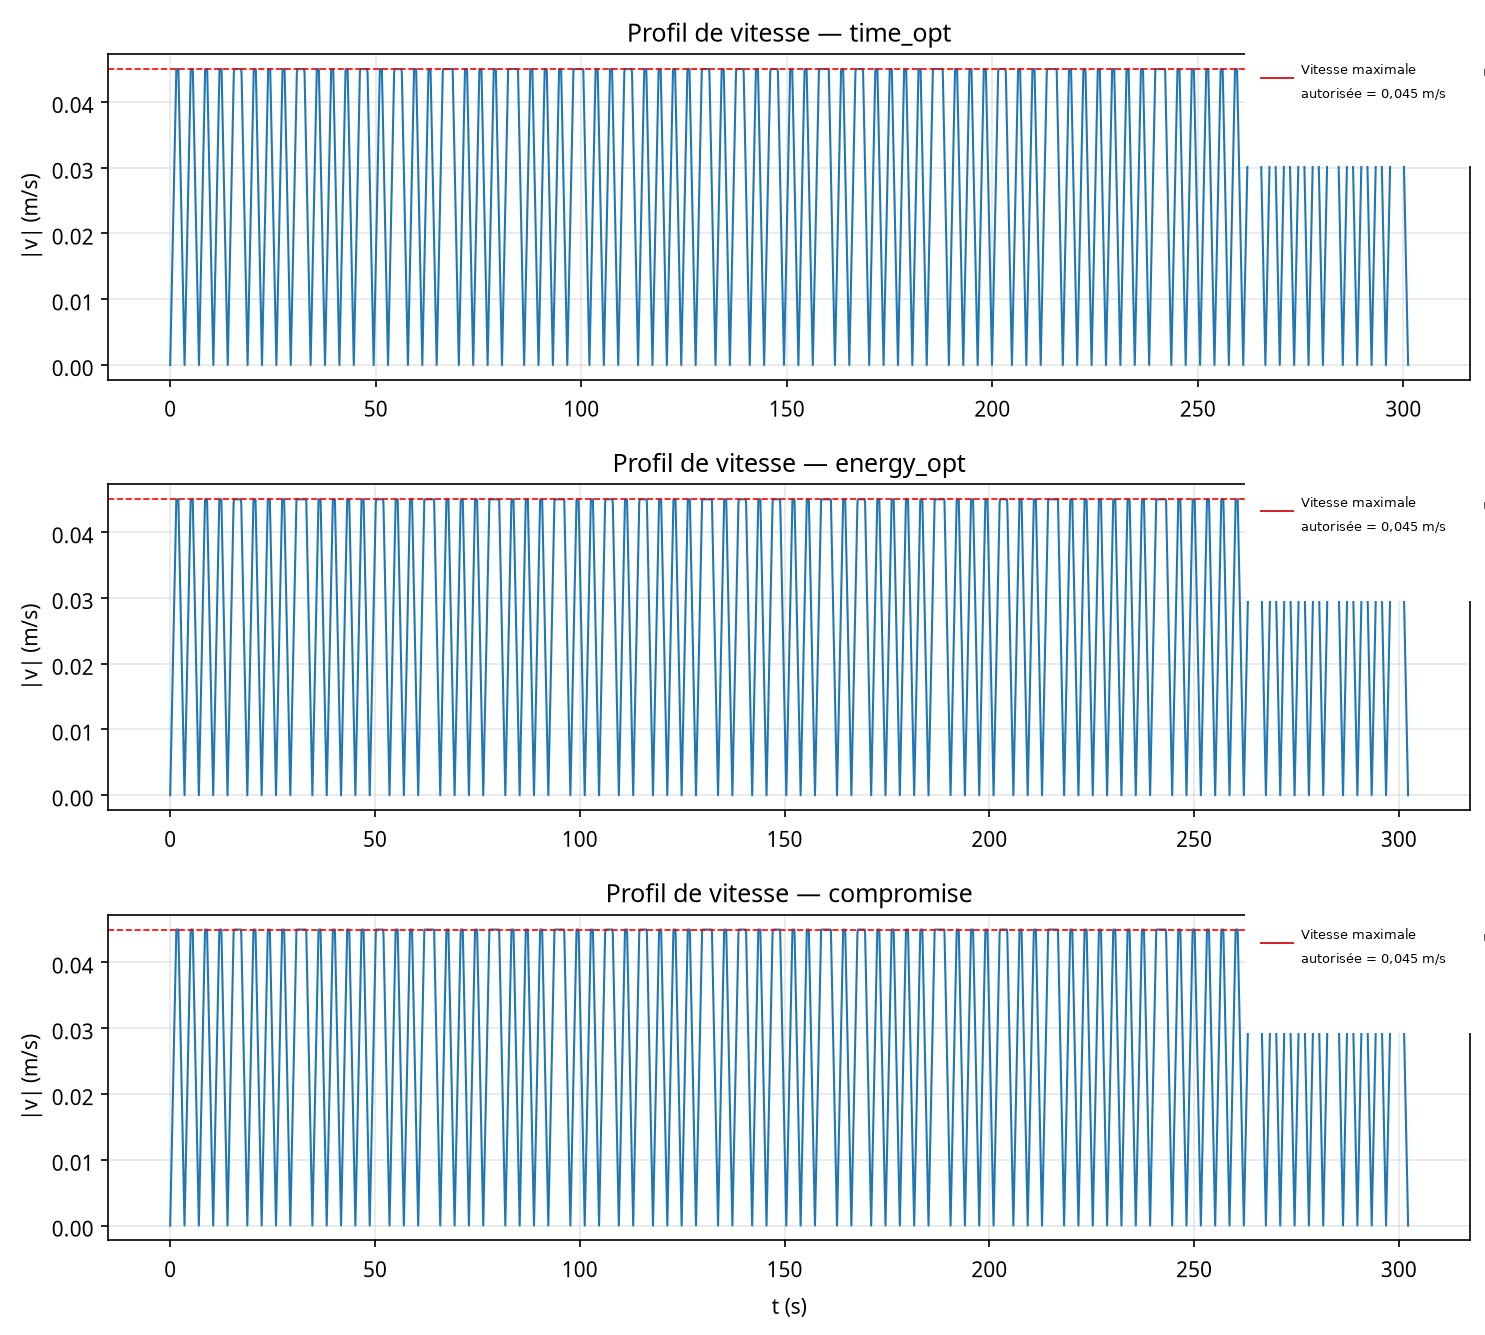
\includegraphics[width=0.92\textwidth,height=0.34\textheight,keepaspectratio]{prof_9x9.png}
\caption{Profils de vitesse LSPB des trois trajectoires, zone étendue}
\label{fig:prof}
\end{figure}

\begin{table}[H]
\centering
\caption{Comparaison zone sécurisée et zone étendue}
\label{tab:zones}
\footnotesize
\begin{tabular}{|c|c|c|c|c|c|}
\hline
\textbf{Grille} & \textbf{Zone} & \textbf{Points} & \textbf{Temps (s)} & \textbf{Énergie (J)} & \textbf{Total (s)} \\
\hline
$7\times7$ & Sécurisée & 49 & 177,30 & 246,44 & 275,3 \\
\hline
$7\times7$ & Étendue & 49 & 191,83 & 314,93 & 289,8 \\
\hline
$9\times9$ & Sécurisée & 81 & 247,04 & 294,09 & 409,0 \\
\hline
$9\times9$ & Étendue & 77 & 301,15 & 636,65 & 455,2 \\
\hline
\end{tabular}
\end{table}

Pour la grille $7\times7$, l'extension ajoute 8,2~\% de temps et 28~\% d'énergie. Pour la grille $9\times9$, elle ajoute 22~\% de temps et 116~\% d'énergie. La zone sécurisée est retenue comme zone de service.

\section{Discussion et perspectives}

\subsection{Limites}

Résultats issus de simulations (câbles rigides, pas de vent, énergie quasi-statique). Paramètres à confirmer : masse opérationnelle, $T_{\max}=58$~N, stabilisation de 2~s. WFW étudié uniquement au plan $z=0{,}45$~m. Robustesse évaluée sur trois graines. Front de Pareto réduit en zone sécurisée. Aucune validation sur prototype.

\subsection{Perspectives}

\begin{itemize}
\item Préciser la courbe énergie--étendue par des bornes intermédiaires.
\item Calculer les tensions maximales minimales sur les zones étendues.
\item Augmenter le nombre de graines pour des tests statistiques.
\item Valider sur le prototype du SP1.
\item Intégrer une replanification en temps réel.
\end{itemize}

\section*{Conclusion}

Ce chapitre a présenté l'architecture du robot Tandem, sa chaîne de traitement en quatre macro-blocs et le dimensionnement de NSGA-II (50 exécutions + 12 de robustesse). Paramètres retenus : 500 individus / 2000 générations ($7\times7$) et 600 / 5000 ($9\times9$).

Sur la zone sécurisée, les trajectoires optimisées réduisent le temps de 22,7~\% ($7\times7$) et 21,0~\% ($9\times9$), et l'énergie de 27,6~\% et 28,7~\%. Les tensions restent sous 58~N (maximum 35,7~N). L'extension de la zone augmente fortement l'énergie (+28~\% / +116~\%). La zone sécurisée constitue un bon compromis pour la mission envisagée. La confirmation passera par une validation sur prototype.


% -------------------- Conclusion générale --------------------
\chapter*{Conclusion générale}
\addcontentsline{toc}{chapter}{Conclusion générale}
\markboth{Conclusion générale}{Conclusion générale}

Ce mémoire, réalisé dans le cadre du projet Tandem, portait sur la planification des trajectoires d'un robot parallèle à câbles destiné à la surveillance du stress hydrique des cultures. L'objectif était de définir un parcours de prise de vue qui couvre la parcelle, respecte les limites mécaniques du robot et réduit le temps de déplacement ainsi que l'énergie mécanique.

Après avoir posé le cadre théorique des robots à câbles et des méthodes d'optimisation multi-objectif, le travail a appliqué l'algorithme NSGA-II au robot Tandem à 8 câbles, au moyen d'une chaîne de traitement en quatre blocs implémentée en Python. Le dimensionnement de l'algorithme, fondé sur 50 exécutions et 12 exécutions de robustesse, a conduit à retenir 500 individus et 2000 générations pour la grille $7\times7$, et 600 individus et 5000 générations pour la grille $9\times9$.

Sur la zone de service sécurisée, tous les points sont atteignables et les tensions restent inférieures à la borne de 58~N (maximum de 35,7~N). Par rapport à un parcours en zigzag, les trajectoires optimisées réduisent le temps de déplacement de 22,7~\% (grille $7\times7$) et de 21,0~\% (grille $9\times9$), et l'énergie mécanique de 27,6~\% et de 28,7~\%. L'extension de la zone de travail est en revanche pénalisante : elle augmente l'énergie de 28~\% et de 116~\% selon la grille, et fait perdre quatre points en $9\times9$. La zone sécurisée est donc retenue.

Ces résultats restent issus de simulations, avec des câbles rigides, sans vent et avec une énergie quasi-statique. La robustesse n'a été évaluée que sur trois graines et les tensions n'ont pas été calculées sur les zones étendues. Les perspectives consistent à consolider l'étude numérique, à valider les trajectoires sur le prototype du SP1, puis à intégrer une replanification en temps réel. Les trajectoires obtenues constituent l'entrée du SP3, chargé de l'analyse des images.


% -------------------- Annexe --------------------
\clearpage
\pagenumbering{roman}
\setcounter{page}{10}% x, xi, xii, ... jusqu'à la fin
\clearpage

\chapter*{Annexe}
\addcontentsline{toc}{chapter}{Annexe}
\thispagestyle{plain}
\markboth{}{}

\renewcommand{\lstlistingname}{Listing}
\setcounter{lstlisting}{0}
\renewcommand{\thelstlisting}{\arabic{lstlisting}}
\captionsetup[lstlisting]{labelsep=space}

\lstset{
  language=Python,
  basicstyle=\ttfamily\footnotesize,
  keywordstyle=\bfseries,
  commentstyle=\itshape\color{gray},
  stringstyle=\color{black},
  showstringspaces=false,
  breaklines=true,
  breakatwhitespace=true,
  frame=single,
  framesep=3pt,
  xleftmargin=0.4em,
  xrightmargin=0.4em,
  aboveskip=0.4em,
  belowskip=0.4em,
  columns=fullflexible,
  keepspaces=true,
  tabsize=4,
  literate=
    {é}{{\'e}}1 {è}{{\`e}}1 {ê}{{\^e}}1 {à}{{\`a}}1
    {ù}{{\`u}}1 {ç}{{\c{c}}}1 {ô}{{\^o}}1
}

\vspace{-0.5em}
Cette annexe présente les extraits de code qui correspondent aux algorithmes décrits au Chapitre~III. Seuls les traitements algorithmiques sont reproduits ; les fonctions de lecture, de journalisation et de sauvegarde sont omises. Le code complet est accessible sur le dépôt indiqué en section~5.

\section*{1 Paramétrage et génération de la grille}
\vspace{-0.3em}
Cette partie décrit le passage des paramètres géométriques à la liste structurée des points de prise de vue.

\paragraph{Principe.}
La configuration est la source unique des dimensions de la grille et des limites opérationnelles. Pour une grille centrée, les coordonnées sont calculées symétriquement autour de l'origine. Chaque point reçoit ensuite un identifiant déterministe selon la relation $\mathrm{id} = \mathrm{ligne} \times n_{\mathrm{colonnes}} + \mathrm{colonne}$, où la ligne repère la position en $Y$ et la colonne la position en $X$. Cette convention est identique à celle utilisée par les blocs de filtrage et de calcul de coûts en aval.

\begin{lstlisting}[caption={Construction deterministe des coordonnees et des identifiants des points},label={lst:B1}]
# Extrait adapte de src/config.py et src/point_generator.py
@dataclass(frozen=True)
class Config:
    # Valeurs du calcul de reference (Chapitre III)
    n_rangs: int = 7            # 9 par defaut dans le depot
    n_colonnes: int = 7         # 9 par defaut dans le depot
    esp_x: float = 0.1333       # 0.20 par defaut dans le depot
    esp_y: float = 0.0800       # 0.20 par defaut dans le depot
    x_min: float = -0.40
    x_max: float = +0.40
    y_min: float = -0.24
    y_max: float = +0.24

def _grid_coordinates(self, origin="centre"):
    cx, cy = (0.0, 0.0) if origin == "centre" else origin
    hx = (self.config.n_colonnes - 1) / 2 * self.config.esp_x
    hy = (self.config.n_rangs - 1) / 2 * self.config.esp_y
    xs = np.linspace(cx - hx, cx + hx, self.config.n_colonnes)
    ys = np.linspace(cy - hy, cy + hy, self.config.n_rangs)
    return xs, ys

def generate(self, origin="centre"):
    xs, ys = self._grid_coordinates(origin)
    rows = []
    for i, y in enumerate(ys):
        for j, x in enumerate(xs):
            rows.append({"id": i*self.config.n_colonnes + j,
                         "x": float(x), "y": float(y),
                         "z": float(self.config.z_absolu_r0),
                         "ligne": i, "colonne": j})
    df = pd.DataFrame(rows)
    self._verify_extent(df)
    return df
\end{lstlisting}

\paragraph{Convention de numérotation.}
L'identifiant suit la relation $\mathrm{id} = \mathrm{ligne} \times 7 + \mathrm{colonne}$ :
\begin{itemize}[itemsep=1pt,topsep=2pt]
\item $\mathrm{id} = 0$ correspond à (ligne~$0$, colonne~$0$), soit $(x = -0{,}400\,;\, y = -0{,}240)$.
\item $\mathrm{id} = 24$ correspond à (ligne~$3$, colonne~$3$), soit le centre $(x = 0\,;\, y = 0)$.
\item $\mathrm{id} = 48$ correspond à (ligne~$6$, colonne~$6$), soit $(x = +0{,}400\,;\, y = +0{,}240)$.
\end{itemize}
Un contrôle d'étendue est effectué après la génération afin de détecter toute incohérence entre les paramètres de grille et les bornes opérationnelles. Le tableau obtenu constitue l'entrée du bloc de filtrage.

\section*{2 Vérification de la faisabilité mécanique par le WFW}
\vspace{-0.3em}
Le WFW (Wrench-Feasible Workspace) décide si une pose admet une distribution de tensions compatible avec l'équilibre statique du robot. La même fonction sert au filtrage et à la validation, afin d'éviter deux définitions concurrentes de la faisabilité.

\paragraph{Formulation.}
Pour une pose $\mathbf{p}$, la matrice de structure $\mathbf{W}(\mathbf{p})$ relie les tensions des huit câbles au torseur extérieur. Le programme résout un problème de faisabilité linéaire sous contraintes d'équilibre et de bornes de tension (équation~III.4) : $\mathbf{W}(\mathbf{p})\,\mathbf{T} = \mathbf{rhs}$, avec $T_{\min} \leq T_i \leq T_{\max}$. Une solution n'est retenue que si le résidu numérique reste inférieur à la tolérance de $10^{-6}$.

\begin{lstlisting}[caption={Test de faisabilite d'une pose par programmation lineaire},label={lst:B2}]
# Extrait adapte de src/wfw.py
class WFW:
    def __init__(self, robot, config):
        self.robot = robot
        self.config = config
        self._rhs = np.array([0., 0., config.masse_kg*9.81,
                              0., 0., 0.])
        self._bounds = [(config.T_min, config.T_max)] * 8

    def is_feasible(self, p):
        W = self.robot.structure_matrix(p)
        if np.linalg.matrix_rank(W) < 6:
            return WFWSolution(False, None, np.nan, -1,
                               "matrice W singuliere")
        res = linprog(np.zeros(8), A_eq=W, b_eq=self._rhs,
                      bounds=self._bounds, method="highs")
        if res.status == 0 and res.x is not None:
            T = np.asarray(res.x, dtype=float)
            residual = float(np.linalg.norm(W @ T - self._rhs))
            if residual <= 1e-6:
                return WFWSolution(True, T, residual, 0,
                                   str(res.message))
        return WFWSolution(False, None, np.nan, int(res.status),
                           str(res.message))
\end{lstlisting}

Le test de rang préalable (\texttt{matrix\_rank(W) < 6}) traite explicitement le cas des plateformes carrées, pour lesquelles la sixième ligne de $\mathbf{W}$ est nulle (la section sur le choix de modélisation). La fonction renvoie une décision booléenne, les tensions lorsque la pose est faisable, le résidu d'équilibre et le statut du solveur. Cette structure permet de distinguer une pose atteignable d'une pose rejetée et de conserver la cause du rejet dans les rapports JSON.

\section*{3 Calcul du temps et de l'énergie de déplacement}
\vspace{-0.3em}
Le bloc de calcul des coûts transforme les points retenus en une matrice de transitions. Chaque paire de points reçoit une distance, un temps de déplacement, une énergie et un indicateur de faisabilité. Cette matrice alimente l'optimisation des tournées.

\paragraph{Temps LSPB et énergie par sous-pas.}
Le temps suit un profil LSPB : trapézoïdal lorsque la distance permet d'atteindre la vitesse maximale, triangulaire dans le cas contraire (équations~III.13 et~III.14). L'énergie est intégrée sur $K$ sous-pas :
\[
E(i,j) = \sum_{k=1}^{K} \sum_{a=1}^{8} T_a(k) \cdot |\Delta L_a(k)|
\]
où $T_a(k)$ est la tension du câble $a$ au milieu du sous-segment $k$ et $\Delta L_a(k)$ la variation de longueur de ce câble sur le sous-segment. Évaluer les tensions aux points milieux préserve la symétrie entre les deux sens de déplacement. La fonction \texttt{\_solve\_tension} applique la résolution en deux chemins décrite en la section sur le choix de modélisation.

\begin{lstlisting}[caption={Calcul du temps LSPB et integration quasi-statique de l'energie},label={lst:B3}]
# Extrait adapte de src/cost_calculator.py
def lspb_time(self, distance):
    if distance <= 0.0:
        return 0.0
    vmax, amax = self.config.v_max, self.config.a_max
    d_acc = vmax*vmax/(2*amax)
    if distance >= 2*d_acc:
        return 2*vmax/amax + (distance - 2*d_acc)/vmax
    v_peak = np.sqrt(distance*amax)
    return 2*v_peak/amax

def _segment_energy(self, p_i, p_j, K=10):
    alphas = np.linspace(0., 1., K+1)
    poses = np.array([p_i + a*(p_j - p_i) for a in alphas])
    lengths = np.array([self.robot.cable_lengths(p) for p in poses])
    dL = np.diff(lengths, axis=0)
    mids = (np.arange(K) + 0.5)/K
    energy, T_prev = 0.0, None
    for k, alpha in enumerate(mids):
        p = p_i + alpha*(p_j - p_i)
        T, ok = self._solve_tension(
            self.robot.structure_matrix(p), T0=T_prev)
        if not ok or T is None:
            return np.nan, False
        energy += float(np.sum(T*np.abs(dL[k])))
        T_prev = T
    return energy, True
\end{lstlisting}

L'énergie d'une transition dépend ainsi de la géométrie du robot, de la variation des longueurs de câbles et de la distribution de tensions admissible. Une liaison dont un sous-pas est infaisable est marquée comme infaisable dans la matrice.

\section*{4 Optimisation multiobjectif par NSGA-II}
\vspace{-0.3em}
Le bloc d'optimisation recherche les tournées qui minimisent simultanément le temps de déplacement et l'énergie. Une tournée est codée comme une permutation des $48$ points non centraux (équation~III.11) ; le centre est imposé au départ et au retour.

\paragraph{Reindexation du centre.}
Dans les matrices internes du problème NSGA-II, le centre est réindexé en position~$0$, quelle que soit sa position dans la grille d'origine (id~$24$ pour la grille $7\times7$). Les gènes $0$ à $47$ désignent alors les positions $1$ à $48$. Cette reindexation est effectuée par le décodage $[0,\, x{+}1,\, 0]$ : les valeurs $0$ aux extrémités correspondent au centre, et les gènes incrémentés de~$1$ correspondent aux points non centraux.

\paragraph{Évaluation d'un chromosome.}
Une solution contenant une liaison infaisable reçoit une pénalité élevée sur les deux objectifs. Les solutions faisables sont évaluées à partir de la matrice de coûts (équation~III.12), puis un post-filtrage strict élimine les solutions dominées à tolérance numérique près.

\begin{lstlisting}[caption={Codage d'une tournee et evaluation multiobjectif par NSGA-II},label={lst:B4}]
# Extrait adapte de src/optimizer.py
class TourProblem(Problem):
    def _decode_positions(self, x):
        x = np.asarray(x, dtype=int)
        # 0 aux extremites = centre ; x+1 = positions 1..n
        return np.concatenate([[0], x + 1, [0]])

    def _evaluate(self, X, out, *args, **kwargs):
        F = np.zeros((len(X), 2), dtype=float)
        for k, chromosome in enumerate(X):
            pos = self._decode_positions(chromosome)
            i, j = pos[:-1], pos[1:]
            feasible = self.feasible_mat[i, j]
            if feasible.all():
                F[k, 0] = self.time_mat[i, j].sum()
                F[k, 1] = self.energy_mat[i, j].sum()
            else:
                penalty = 1e6 * (1 + int((~feasible).sum()))
                F[k, :] = penalty
        out["F"] = F

algorithm = NSGA2(
    pop_size=pop_size,
    sampling=PermutationRandomSampling(),
    crossover=OrderCrossover(),
    mutation=InversionMutation(),
    eliminate_duplicates=True)
res = minimize(problem, algorithm, ("n_gen", n_gen),
               seed=seed, verbose=False)
\end{lstlisting}

Le front de Pareto rassemble les solutions non dominées selon les deux critères. Pour le calcul de référence, la taille de population ($500$ individus), le nombre de générations ($5000$) et la graine ($42$) sont fixés explicitement afin de garantir la reproductibilité.

\clearpage\section*{5 Enchaînement du pipeline et production des résultats}
\vspace{-0.3em}
Le script d'exécution assemble les blocs précédents. L'extrait ci-dessous résume l'ordre de traitement. Il omet l'analyse de la ligne de commande (dont l'option \texttt{--zero-loss}), la journalisation et la sauvegarde détaillée.

\begin{lstlisting}[caption={Sequence generale d'execution du pipeline Tandem},label={lst:5}]
# Extrait synthetique de scripts/run_pipeline.py
config = Config.with_n(7)
robot = RobotModel(config)
wfw = WFW(robot, config)
# Bloc 4 : generation des points
points = PointGenerator(config).generate()
# Bloc 5 : conservation des poses atteignables
filtered = PointFilter(config, wfw).filter(points)
df_points = filtered.points_retenus
# Bloc 6 : matrice des couts entre points retenus
costs = CostCalculator(config, robot).build_matrix(
    df_points, K=10)
# Bloc 7 : optimisation multiobjectif
solutions, result = Optimizer(
    config, df_points, costs).run(
        pop_size=500, n_gen=5000, seed=42)
# Bloc 8 : selection et reconstruction des trajectoires
extracted = TrajectoryExtractor(
    config, df_points, costs, solutions).run()\end{lstlisting}

\vspace{-1.0em}
\begin{samepage}
\noindent Dépôt du projet Tandem : \url{https://github.com/safidinjarahenrialvin/tandem_sp2}
\hfill
\includegraphics[width=1.5cm]{figures/qrcode_tandem_sp2.png}

\noindent Ces extraits mettent en évidence les choix algorithmiques essentiels : génération déterministe de la grille, faisabilité mécanique par programmation linéaire, calcul énergétique sous contraintes et optimisation multiobjectif. Les détails répétitifs de formatage et d'export sont volontairement exclus.
\end{samepage}


% -------------------- Bibliographie --------------------
\clearpage
\bibliographystyle{plain}
% Si vous utilisez references.bib avec BibTeX, décommentez :
% \bibliography{references}
% Version actuelle : bibliographie manuelle
\begin{thebibliography}{99}
\addcontentsline{toc}{chapter}{Bibliographie}

\bibitem{dahiya2022}
Dahiya A. et al., \textit{Adaptive Passivity-Based Pose Tracking Control of Cable-Driven Parallel Robots for Multiple Attitude Parameterizations}, arXiv:2209.03250.

\bibitem{tho2022}
Tho T.P. et al., \textit{An Overview of Cable-Driven Parallel Robots: Workspace, Tension Distribution, and Cable Sagging}, Mathematical Problems in Engineering, Hindawi, 2022.

\bibitem{gouttefarde2011}
Gouttefarde M. et al., \textit{Interval analysis for the Wrench-Feasible Workspace of Cable-Driven Parallel Robots}, 2011.

\bibitem{mdpi2022}
\textit{Cable-Driven Parallel Robots: A Systematic Review}, MDPI, 2022.

\bibitem{mdpi2023}
\textit{Advances in Cable-Driven Parallel Robots}, MDPI, 2023.

\bibitem{arXiv2101}
\textit{Cable-Driven Parallel Robot Modeling and Control}, arXiv:2101.xxxxx.

\bibitem{arXiv2311}
\textit{Trajectory Planning for Cable Robots}, arXiv:2311.xxxxx.

\bibitem{arXiv2403}
\textit{Multi-Objective Optimization of CDPR Trajectories}, arXiv:2403.xxxxx.

\bibitem{liu2023}
Liu et al., \textit{Path Planning Methods for Parallel Robots}, 2023.

\bibitem{gasparetto2015}
Gasparetto A. et al., \textit{Path Planning and Trajectory Planning Algorithms: A General Overview}, 2015.

\bibitem{choset1998}
Choset H., Pignon P., \textit{Coverage Path Planning: The Boustrophedon Cellular Decomposition}, 1998.

\bibitem{duan2014}
Duan et al., \textit{TSP and Vehicle Routing for Mobile Robots}, 2014.

\bibitem{lspb}
\textit{Linear Segments with Parabolic Blends (LSPB) Trajectory Profiles}.

\bibitem{zhang2024}
Zhang et al., \textit{Trajectory Smoothing for Robotic Systems}, 2024.

\bibitem{deb2002}
Deb K. et al., \textit{A Fast and Elitist Multiobjective Genetic Algorithm: NSGA-II}, IEEE TEC, 2002.

\bibitem{khayour2022}
Khayour et al., \textit{Robust Control of Cable-Driven Parallel Robots}, 2022.

\bibitem{puphal2026}
Puphal et al., \textit{Uncertainty Management in Robotic Trajectory Planning}, 2026.

\end{thebibliography}

% -------------------- Annexes (optionnel) --------------------
% \clearpage
% Numérotation romaine pour annexe et bibliographie
\pagenumbering{roman}
\setcounter{page}{11}

\chapter*{Annexe A}
\addcontentsline{toc}{chapter}{Annexe A}
\thispagestyle{plain}
\markboth{}{}
% Numérotation des tableaux de l'annexe : A.1, A.2, …
\setcounter{table}{0}
\renewcommand{\thetable}{A.\arabic{table}}

Cette annexe rassemble les données géométriques, matérielles et numériques qui complètent le Chapitre~III et permettent de reproduire le calcul.

\section*{A.1 Géométrie et matériel de référence}

\subsection*{A.1.1 Ancrages et attaches}

Le tableau~A.1 donne les coordonnées des ancrages $\mathbf{A}_i$, exprimées dans le repère fixe $R_0$, et celles des attaches $\mathbf{b}_i$, exprimées dans le repère de la plateforme ($300 \times 240$~mm, orientation fixe $R = I$). Les câbles 1 à 4 sont les câbles hauts et les câbles 5 à 8 les câbles bas. Les câbles 2 à 4 et 6 à 8 sont numérotés par symétrie à partir des câbles 1 et 5.

\begin{table}[H]
\centering
\caption{Coordonnées des ancrages $\mathbf{A}_i$ ($R_0$) et des attaches $\mathbf{b}_i$ (plateforme), en mètres}
\label{tab:A1}
\footnotesize
\begin{tabular}{|c|c|c|c|c|c|c|}
\hline
\textbf{Câble} & $\mathbf{A}_{ix}$ & $\mathbf{A}_{iy}$ & $\mathbf{A}_{iz}$ & $\mathbf{b}_{ix}$ & $\mathbf{b}_{iy}$ & $\mathbf{b}_{iz}$ \\
\hline
1 & $-1{,}25$ & $+1{,}25$ & $+1{,}00$ & $-0{,}150$ & $+0{,}120$ & $+0{,}025$ \\
\hline
2 & $+1{,}25$ & $+1{,}25$ & $+1{,}00$ & $+0{,}150$ & $+0{,}120$ & $+0{,}025$ \\
\hline
3 & $-1{,}25$ & $-1{,}25$ & $+1{,}00$ & $-0{,}150$ & $-0{,}120$ & $+0{,}025$ \\
\hline
4 & $+1{,}25$ & $-1{,}25$ & $+1{,}00$ & $+0{,}150$ & $-0{,}120$ & $+0{,}025$ \\
\hline
5 & $-1{,}25$ & $+1{,}25$ & $0{,}00$ & $-0{,}150$ & $+0{,}120$ & $-0{,}025$ \\
\hline
6 & $+1{,}25$ & $+1{,}25$ & $0{,}00$ & $+0{,}150$ & $+0{,}120$ & $-0{,}025$ \\
\hline
7 & $-1{,}25$ & $-1{,}25$ & $0{,}00$ & $-0{,}150$ & $-0{,}120$ & $-0{,}025$ \\
\hline
8 & $+1{,}25$ & $-1{,}25$ & $0{,}00$ & $+0{,}150$ & $-0{,}120$ & $-0{,}025$ \\
\hline
\end{tabular}
\end{table}

Pour une pose $\mathbf{p}$, l'attache exprimée dans $R_0$ vaut $\mathbf{B}_i(\mathbf{p}) = \mathbf{p} + \mathbf{b}_i$ et la longueur du câble est $l_i = \|\mathbf{A}_i - \mathbf{B}_i(\mathbf{p})\|$ (équation~III.1). À la position centrale $\mathbf{p} = (0\,;\, 0\,;\, 0{,}45)$~m, le câble~1 donne $l_1 = 1{,}662$~m, valeur reprise au tableau~III.4.

\subsection*{A.1.2 Actionneurs et transmission}

Le tableau~A.2 précise les composants qui interviennent dans la borne $T_{\max} = 58$~N du Chapitre~III.

\begin{table}[H]
\centering
\caption{Spécifications matérielles}
\label{tab:A2}
\footnotesize
\begin{tabular}{|p{3.6cm}|p{3.4cm}|p{5.2cm}|}
\hline
\textbf{Composant} & \textbf{Paramètre} & \textbf{Valeur} \\
\hline
Moteur pas à pas NEMA~17 & Couple de maintien & $0{,}40$ à $0{,}47$~N$\cdot$m \\
\cline{2-3}
 & Angle de pas & $1{,}8^\circ$ (200 pas/tour) \\
\cline{2-3}
 & Courant par phase & $1{,}5$ à $1{,}7$~A \\
\hline
Tambour & Diamètre / rayon & $80$~mm / $40$~mm \\
\cline{2-3}
 & Enroulement par tour & $0{,}2513$~m \\
\hline
Câble Dyneema & Diamètre & $4$~mm \\
\cline{2-3}
 & Module d'Young & $80$ à $120$~GPa \\
\cline{2-3}
 & Charge de rupture & $> 500$~N \\
\hline
Poulie & Type / rayon & articulée (type WZ~31) / $20$~mm \\
\hline
\end{tabular}
\end{table}

\paragraph{Justification de $T_{\max}$.}
La tension qu'un actionneur peut exercer vaut $T = C / r$, où $C$ est le couple disponible au tambour et $r$ son rayon. Sur un tambour de $40$~mm et sans réduction, un couple de $0{,}47$~N$\cdot$m donne $T \approx 11{,}8$~N. La borne $T_{\max} = 58$~N retenue pour le calcul suppose donc une réduction d'environ $5{:}1$ entre le moteur et le tambour. Elle est utilisée comme borne supérieure de dimensionnement. Le calcul de référence n'en dépend pas : les tensions maximales obtenues ($4{,}395$~N) restent inférieures à la capacité du moteur en entraînement direct.

Le rapport entre la charge de rupture du câble et $T_{\max}$ dépasse $8$, ce qui laisse une large marge de sécurité. Le modèle de câble reste idéal (inextensible, sans masse) : l'élasticité, la flèche et le frottement de poulie ne sont pas pris en compte (voir~A.7).

\section*{A.2 Configuration du calcul et grille des points de vue}

\subsection*{A.2.1 Commande de référence}

Tous les résultats du Chapitre~III proviennent d'un seul calcul :
\begin{verbatim}
python scripts/run_pipeline.py --n 7 --zero-loss --pop-size 500 \
    --n-gen 5000 --output-dir data/outputs_7x7_pop500_gen5000 --verbose
\end{verbatim}

Les options de la commande priment sur la configuration par défaut : la grille est de $7\times7$ ($N = 49$). La graine du générateur aléatoire est $42$, ce qui rend l'optimisation NSGA-II déterministe. Les fichiers produits (CSV et JSON) sont conservés dans l'archive du calcul et se régénèrent avec cette commande.

\begin{table}[H]
\centering
\caption{Paramètres complémentaires du calcul}
\label{tab:A3}
\footnotesize
\begin{tabular}{|l|p{4.0cm}|p{6.5cm}|}
\hline
\textbf{Famille} & \textbf{Paramètre} & \textbf{Valeur} \\
\hline
Mission & Hauteur de prise de vue & $0{,}45$~m dans $R_0$ ($z_{\mathrm{vol}} = 0{,}30$~m, plants $0{,}35$~m, offset sol $0{,}20$~m) \\
\hline
Mission & Stabilisation par point & $2$~s ($49 \times 2 = 98$~s au total) \\
\hline
Vision & Champ de vue de la caméra & $62{,}2^\circ \times 48{,}8^\circ$ \\
\hline
Cinématique & $a_{\max}$ & $0{,}030$~m/s$^2$ \\
\hline
Cinématique & $T_{\mathrm{acc}} / T_{\mathrm{dec}}$ (profil LSPB) & $1{,}5$~s / $1{,}5$~s \\
\hline
NSGA-II & Opérateurs & croisement OX, mutation par inversion \\
\hline
\end{tabular}
\end{table}

\subsection*{A.2.2 Grille des points de vue}

Les $49$ points sont répartis uniformément dans le plan $z = 0{,}45$~m :
\begin{equation*}
x_k = -0{,}400 + k \times 0{,}1333~\text{m},
\qquad
y_m = -0{,}240 + m \times 0{,}0800~\text{m},
\quad k, m \in \{0, \ldots, 6\}.
\end{equation*}
Le pas est donc de $0{,}1333$~m selon $X$ et de $0{,}0800$~m selon $Y$. Le point~$0$ est $(-0{,}400\,;\, -0{,}240\,;\, 0{,}450)$. Le centre (id~$24$), point de départ et de retour de la mission, est $(0\,;\, 0\,;\, 0{,}450)$. Le point~$48$ est $(+0{,}400\,;\, +0{,}240\,;\, 0{,}450)$.

L'empreinte de la caméra à $0{,}45$~m est d'environ $0{,}3619 \times 0{,}2722$~m. Les recouvrements entre points voisins sont de $0{,}2286$~m en $X$ et $0{,}1922$~m en $Y$, ce qui assure une couverture complète. Les $49$ points sont tous retenus par le filtrage (aucun rejet, pour un seuil configuré de $15\,\%$).

\section*{A.3 Hypothèses de modélisation}

Cinq hypothèses ont été figées pour le calcul.

\begin{table}[H]
\centering
\caption{Hypothèses B1 à B5}
\label{tab:A4}
\footnotesize
\begin{tabular}{|c|p{3.8cm}|p{2.8cm}|p{4.5cm}|}
\hline
\textbf{Code} & \textbf{Hypothèse} & \textbf{Valeur} & \textbf{Statut} \\
\hline
B1 & Masse opérationnelle & $0{,}383988$~kg & Estimation calibrée ; à confirmer par pesée \\
\hline
B2 & Hauteur des plants & $0{,}35$~m & Estimation pour un haricot nain ; à mesurer \\
\hline
B3 & Champ de vue de la caméra & $62{,}2^\circ \times 48{,}8^\circ$ & Valeur constructeur \\
\hline
B4 & Grille et effectif & $7\times7$ ; $N = 49$ & Validée par le WFW sur les $49$ points \\
\hline
B5 & Offset sol / $R_0$ & $0{,}20$~m & Confirmé par le montage \\
\hline
\end{tabular}
\end{table}

\section*{A.4 Statistiques de la matrice de coûts}

La matrice contient $49 \times 49 = 2401$ entrées. La diagonale est nulle, toutes les paires sont réalisables et les valeurs sont symétriques dans les tolérances du validateur.

\begin{table}[H]
\centering
\caption{Statistiques (toutes paires ordonnées, diagonale incluse)}
\label{tab:A5}
\begin{tabular}{|l|c|c|c|}
\hline
\textbf{Statistique} & \textbf{Distance (m)} & \textbf{Temps (s)} & \textbf{Énergie (J)} \\
\hline
Minimum & $0{,}000$ & $0{,}000$ & $0{,}000$ \\
\hline
Médiane & $0{,}400$ & $10{,}389$ & $14{,}612$ \\
\hline
Moyenne & $0{,}391$ & $10{,}163$ & $15{,}431$ \\
\hline
Maximum & $0{,}933$ & $22{,}232$ & $49{,}240$ \\
\hline
\end{tabular}
\end{table}

Ces valeurs concernent des déplacements élémentaires entre deux points. Elles ne correspondent pas aux cumuls d'une trajectoire complète, qui dépendent de l'ordre de visite.

\section*{A.5 Validation logicielle}

Six contrôles sur sept sont réussis, un donne un avertissement et aucun n'échoue (tableau~A.6).

\begin{table}[H]
\centering
\caption{Résultats de validation}
\label{tab:A6}
\footnotesize
\begin{tabular}{|p{3.6cm}|c|p{7.2cm}|}
\hline
\textbf{Contrôle} & \textbf{Statut} & \textbf{Évidence} \\
\hline
Cohérence de la configuration & PASS & $N = 49$ ; $T \in [1\,;\, 58]$~N ; orientation fixe \\
\hline
Points filtrés & PASS & $49$ points ; aucun infaisable \\
\hline
Matrice de coûts & PASS & $2401$ entrées ; symétrie ; diagonale nulle \\
\hline
Solutions de Pareto & WARN & Une solution non dominée unique ; seuil recommandé $\geq 10$ \\
\hline
Trajectoires & PASS & $3$ types ; centre aux extrémités ; totaux cohérents \\
\hline
Profils cinématiques & PASS & $5361$ échantillons ; $\|\mathbf{v}\|_{\max} = 0{,}045$~m/s \\
\hline
Cohérence croisée & PASS & Profils, matrice et résumé concordants \\
\hline
\end{tabular}
\end{table}

\paragraph{Interprétation de l'avertissement.}
Le fichier \texttt{solutions\_pareto.csv} contient deux ordres de visite distincts dont les objectifs sont rigoureusement identiques : ($177{,}295$~s ; $246{,}436$~J). Le validateur les compte comme une seule solution non dominée, d'où $n_{\mathrm{solutions}} = 1$. Il s'agit d'un doublon de représentation du même point objectif, et non d'une incohérence. L'avertissement signale seulement que le front est trop réduit pour étudier un compromis entre temps et énergie.

\section*{A.6 Choix de modélisation}

\paragraph{Convention de signe.}
La direction unitaire est $\mathbf{U}_i = (\mathbf{A}_i - \mathbf{B}_i) / \|\mathbf{A}_i - \mathbf{B}_i\|$, orientée de l'attache vers l'ancrage, c'est-à-dire dans le sens physique de la traction. La matrice de structure $W$ assemble les vecteurs $[\mathbf{U}_i\,;\, \mathbf{B}_i \times \mathbf{U}_i]$. Cette convention évite d'obtenir des tensions positives qui correspondraient en réalité à une compression de la plateforme.

\paragraph{Résolution des tensions en deux chemins.}
À chaque sous-pas, une solution par pseudo-inverse est tentée en premier. Si elle sort de $[T_{\min}\,;\, T_{\max}]$, un solveur borné SLSQP, initialisé par la solution précédente, prend le relais. Le coût de calcul moyen est ainsi réduit sans perdre la robustesse dans les cas limites.

\paragraph{Énergie au point milieu.}
L'énergie de chaque sous-segment est évaluée en son point milieu, ce qui rend $E(i,j)$ et $E(j,i)$ symétriques par construction.

\section*{A.7 Limites et protocole expérimental}

\begin{table}[H]
\centering
\caption{Limites et actions associées}
\label{tab:A7}
\footnotesize
\begin{tabular}{|p{3.8cm}|p{4.2cm}|p{4.5cm}|}
\hline
\textbf{Limite} & \textbf{Impact} & \textbf{Action} \\
\hline
Masse estimée (B1) & Influence le poids et les tensions & Peser la plateforme ; relancer le calcul si l'écart dépasse $5\,\%$ \\
\hline
$T_{\max} = 58$~N & Dépend du couple, de la réduction et du rayon du tambour & Vérifier la chaîne de transmission complète \\
\hline
Absence de vent et de perturbations & Efforts externes non modélisés & Ajouter des scénarios de charge et de replanification \\
\hline
Solution non dominée unique & Pas d'étude statistique du compromis & Répéter avec plusieurs graines \\
\hline
Câble idéal & Élasticité, flèche et frottement négligés & Valider par mesure des tensions \\
\hline
Stabilisation constante ($2$~s) & Indépendante du mouvement et des vibrations & Mesurer le temps réel sur prototype \\
\hline
\end{tabular}
\end{table}


% \clearpage

\chapter*{Annexe}
\addcontentsline{toc}{chapter}{Annexe}
\thispagestyle{plain}
\markboth{}{}

\renewcommand{\lstlistingname}{Listing}
\setcounter{lstlisting}{0}
\renewcommand{\thelstlisting}{\arabic{lstlisting}}
\captionsetup[lstlisting]{labelsep=space}

\lstset{
  language=Python,
  basicstyle=\ttfamily\footnotesize,
  keywordstyle=\bfseries,
  commentstyle=\itshape\color{gray},
  stringstyle=\color{black},
  showstringspaces=false,
  breaklines=true,
  breakatwhitespace=true,
  frame=single,
  framesep=3pt,
  xleftmargin=0.4em,
  xrightmargin=0.4em,
  aboveskip=0.4em,
  belowskip=0.4em,
  columns=fullflexible,
  keepspaces=true,
  tabsize=4,
  literate=
    {é}{{\'e}}1 {è}{{\`e}}1 {ê}{{\^e}}1 {à}{{\`a}}1
    {ù}{{\`u}}1 {ç}{{\c{c}}}1 {ô}{{\^o}}1
}

\vspace{-0.5em}
Cette annexe présente les extraits de code qui correspondent aux algorithmes décrits au Chapitre~III. Seuls les traitements algorithmiques sont reproduits ; les fonctions de lecture, de journalisation et de sauvegarde sont omises. Le code complet est accessible sur le dépôt indiqué en section~5.

\section*{1 Paramétrage et génération de la grille}
\vspace{-0.3em}
Cette partie décrit le passage des paramètres géométriques à la liste structurée des points de prise de vue.

\paragraph{Principe.}
La configuration est la source unique des dimensions de la grille et des limites opérationnelles. Pour une grille centrée, les coordonnées sont calculées symétriquement autour de l'origine. Chaque point reçoit ensuite un identifiant déterministe selon la relation $\mathrm{id} = \mathrm{ligne} \times n_{\mathrm{colonnes}} + \mathrm{colonne}$, où la ligne repère la position en $Y$ et la colonne la position en $X$. Cette convention est identique à celle utilisée par les blocs de filtrage et de calcul de coûts en aval.

\begin{lstlisting}[caption={Construction deterministe des coordonnees et des identifiants des points},label={lst:B1}]
# Extrait adapte de src/config.py et src/point_generator.py
@dataclass(frozen=True)
class Config:
    # Valeurs du calcul de reference (Chapitre III)
    n_rangs: int = 7            # 9 par defaut dans le depot
    n_colonnes: int = 7         # 9 par defaut dans le depot
    esp_x: float = 0.1333       # 0.20 par defaut dans le depot
    esp_y: float = 0.0800       # 0.20 par defaut dans le depot
    x_min: float = -0.40
    x_max: float = +0.40
    y_min: float = -0.24
    y_max: float = +0.24

def _grid_coordinates(self, origin="centre"):
    cx, cy = (0.0, 0.0) if origin == "centre" else origin
    hx = (self.config.n_colonnes - 1) / 2 * self.config.esp_x
    hy = (self.config.n_rangs - 1) / 2 * self.config.esp_y
    xs = np.linspace(cx - hx, cx + hx, self.config.n_colonnes)
    ys = np.linspace(cy - hy, cy + hy, self.config.n_rangs)
    return xs, ys

def generate(self, origin="centre"):
    xs, ys = self._grid_coordinates(origin)
    rows = []
    for i, y in enumerate(ys):
        for j, x in enumerate(xs):
            rows.append({"id": i*self.config.n_colonnes + j,
                         "x": float(x), "y": float(y),
                         "z": float(self.config.z_absolu_r0),
                         "ligne": i, "colonne": j})
    df = pd.DataFrame(rows)
    self._verify_extent(df)
    return df
\end{lstlisting}

\paragraph{Convention de numérotation.}
L'identifiant suit la relation $\mathrm{id} = \mathrm{ligne} \times 7 + \mathrm{colonne}$ :
\begin{itemize}[itemsep=1pt,topsep=2pt]
\item $\mathrm{id} = 0$ correspond à (ligne~$0$, colonne~$0$), soit $(x = -0{,}400\,;\, y = -0{,}240)$.
\item $\mathrm{id} = 24$ correspond à (ligne~$3$, colonne~$3$), soit le centre $(x = 0\,;\, y = 0)$.
\item $\mathrm{id} = 48$ correspond à (ligne~$6$, colonne~$6$), soit $(x = +0{,}400\,;\, y = +0{,}240)$.
\end{itemize}
Un contrôle d'étendue est effectué après la génération afin de détecter toute incohérence entre les paramètres de grille et les bornes opérationnelles. Le tableau obtenu constitue l'entrée du bloc de filtrage.

\section*{2 Vérification de la faisabilité mécanique par le WFW}
\vspace{-0.3em}
Le WFW (Wrench-Feasible Workspace) décide si une pose admet une distribution de tensions compatible avec l'équilibre statique du robot. La même fonction sert au filtrage et à la validation, afin d'éviter deux définitions concurrentes de la faisabilité.

\paragraph{Formulation.}
Pour une pose $\mathbf{p}$, la matrice de structure $\mathbf{W}(\mathbf{p})$ relie les tensions des huit câbles au torseur extérieur. Le programme résout un problème de faisabilité linéaire sous contraintes d'équilibre et de bornes de tension (équation~III.4) : $\mathbf{W}(\mathbf{p})\,\mathbf{T} = \mathbf{rhs}$, avec $T_{\min} \leq T_i \leq T_{\max}$. Une solution n'est retenue que si le résidu numérique reste inférieur à la tolérance de $10^{-6}$.

\begin{lstlisting}[caption={Test de faisabilite d'une pose par programmation lineaire},label={lst:B2}]
# Extrait adapte de src/wfw.py
class WFW:
    def __init__(self, robot, config):
        self.robot = robot
        self.config = config
        self._rhs = np.array([0., 0., config.masse_kg*9.81,
                              0., 0., 0.])
        self._bounds = [(config.T_min, config.T_max)] * 8

    def is_feasible(self, p):
        W = self.robot.structure_matrix(p)
        if np.linalg.matrix_rank(W) < 6:
            return WFWSolution(False, None, np.nan, -1,
                               "matrice W singuliere")
        res = linprog(np.zeros(8), A_eq=W, b_eq=self._rhs,
                      bounds=self._bounds, method="highs")
        if res.status == 0 and res.x is not None:
            T = np.asarray(res.x, dtype=float)
            residual = float(np.linalg.norm(W @ T - self._rhs))
            if residual <= 1e-6:
                return WFWSolution(True, T, residual, 0,
                                   str(res.message))
        return WFWSolution(False, None, np.nan, int(res.status),
                           str(res.message))
\end{lstlisting}

Le test de rang préalable (\texttt{matrix\_rank(W) < 6}) traite explicitement le cas des plateformes carrées, pour lesquelles la sixième ligne de $\mathbf{W}$ est nulle (la section sur le choix de modélisation). La fonction renvoie une décision booléenne, les tensions lorsque la pose est faisable, le résidu d'équilibre et le statut du solveur. Cette structure permet de distinguer une pose atteignable d'une pose rejetée et de conserver la cause du rejet dans les rapports JSON.

\section*{3 Calcul du temps et de l'énergie de déplacement}
\vspace{-0.3em}
Le bloc de calcul des coûts transforme les points retenus en une matrice de transitions. Chaque paire de points reçoit une distance, un temps de déplacement, une énergie et un indicateur de faisabilité. Cette matrice alimente l'optimisation des tournées.

\paragraph{Temps LSPB et énergie par sous-pas.}
Le temps suit un profil LSPB : trapézoïdal lorsque la distance permet d'atteindre la vitesse maximale, triangulaire dans le cas contraire (équations~III.13 et~III.14). L'énergie est intégrée sur $K$ sous-pas :
\[
E(i,j) = \sum_{k=1}^{K} \sum_{a=1}^{8} T_a(k) \cdot |\Delta L_a(k)|
\]
où $T_a(k)$ est la tension du câble $a$ au milieu du sous-segment $k$ et $\Delta L_a(k)$ la variation de longueur de ce câble sur le sous-segment. Évaluer les tensions aux points milieux préserve la symétrie entre les deux sens de déplacement. La fonction \texttt{\_solve\_tension} applique la résolution en deux chemins décrite en la section sur le choix de modélisation.

\begin{lstlisting}[caption={Calcul du temps LSPB et integration quasi-statique de l'energie},label={lst:B3}]
# Extrait adapte de src/cost_calculator.py
def lspb_time(self, distance):
    if distance <= 0.0:
        return 0.0
    vmax, amax = self.config.v_max, self.config.a_max
    d_acc = vmax*vmax/(2*amax)
    if distance >= 2*d_acc:
        return 2*vmax/amax + (distance - 2*d_acc)/vmax
    v_peak = np.sqrt(distance*amax)
    return 2*v_peak/amax

def _segment_energy(self, p_i, p_j, K=10):
    alphas = np.linspace(0., 1., K+1)
    poses = np.array([p_i + a*(p_j - p_i) for a in alphas])
    lengths = np.array([self.robot.cable_lengths(p) for p in poses])
    dL = np.diff(lengths, axis=0)
    mids = (np.arange(K) + 0.5)/K
    energy, T_prev = 0.0, None
    for k, alpha in enumerate(mids):
        p = p_i + alpha*(p_j - p_i)
        T, ok = self._solve_tension(
            self.robot.structure_matrix(p), T0=T_prev)
        if not ok or T is None:
            return np.nan, False
        energy += float(np.sum(T*np.abs(dL[k])))
        T_prev = T
    return energy, True
\end{lstlisting}

L'énergie d'une transition dépend ainsi de la géométrie du robot, de la variation des longueurs de câbles et de la distribution de tensions admissible. Une liaison dont un sous-pas est infaisable est marquée comme infaisable dans la matrice.

\section*{4 Optimisation multiobjectif par NSGA-II}
\vspace{-0.3em}
Le bloc d'optimisation recherche les tournées qui minimisent simultanément le temps de déplacement et l'énergie. Une tournée est codée comme une permutation des $48$ points non centraux (équation~III.11) ; le centre est imposé au départ et au retour.

\paragraph{Reindexation du centre.}
Dans les matrices internes du problème NSGA-II, le centre est réindexé en position~$0$, quelle que soit sa position dans la grille d'origine (id~$24$ pour la grille $7\times7$). Les gènes $0$ à $47$ désignent alors les positions $1$ à $48$. Cette reindexation est effectuée par le décodage $[0,\, x{+}1,\, 0]$ : les valeurs $0$ aux extrémités correspondent au centre, et les gènes incrémentés de~$1$ correspondent aux points non centraux.

\paragraph{Évaluation d'un chromosome.}
Une solution contenant une liaison infaisable reçoit une pénalité élevée sur les deux objectifs. Les solutions faisables sont évaluées à partir de la matrice de coûts (équation~III.12), puis un post-filtrage strict élimine les solutions dominées à tolérance numérique près.

\begin{lstlisting}[caption={Codage d'une tournee et evaluation multiobjectif par NSGA-II},label={lst:B4}]
# Extrait adapte de src/optimizer.py
class TourProblem(Problem):
    def _decode_positions(self, x):
        x = np.asarray(x, dtype=int)
        # 0 aux extremites = centre ; x+1 = positions 1..n
        return np.concatenate([[0], x + 1, [0]])

    def _evaluate(self, X, out, *args, **kwargs):
        F = np.zeros((len(X), 2), dtype=float)
        for k, chromosome in enumerate(X):
            pos = self._decode_positions(chromosome)
            i, j = pos[:-1], pos[1:]
            feasible = self.feasible_mat[i, j]
            if feasible.all():
                F[k, 0] = self.time_mat[i, j].sum()
                F[k, 1] = self.energy_mat[i, j].sum()
            else:
                penalty = 1e6 * (1 + int((~feasible).sum()))
                F[k, :] = penalty
        out["F"] = F

algorithm = NSGA2(
    pop_size=pop_size,
    sampling=PermutationRandomSampling(),
    crossover=OrderCrossover(),
    mutation=InversionMutation(),
    eliminate_duplicates=True)
res = minimize(problem, algorithm, ("n_gen", n_gen),
               seed=seed, verbose=False)
\end{lstlisting}

Le front de Pareto rassemble les solutions non dominées selon les deux critères. Pour le calcul de référence, la taille de population ($500$ individus), le nombre de générations ($5000$) et la graine ($42$) sont fixés explicitement afin de garantir la reproductibilité.

\clearpage\section*{5 Enchaînement du pipeline et production des résultats}
\vspace{-0.3em}
Le script d'exécution assemble les blocs précédents. L'extrait ci-dessous résume l'ordre de traitement. Il omet l'analyse de la ligne de commande (dont l'option \texttt{--zero-loss}), la journalisation et la sauvegarde détaillée.

\begin{lstlisting}[caption={Sequence generale d'execution du pipeline Tandem},label={lst:5}]
# Extrait synthetique de scripts/run_pipeline.py
config = Config.with_n(7)
robot = RobotModel(config)
wfw = WFW(robot, config)
# Bloc 4 : generation des points
points = PointGenerator(config).generate()
# Bloc 5 : conservation des poses atteignables
filtered = PointFilter(config, wfw).filter(points)
df_points = filtered.points_retenus
# Bloc 6 : matrice des couts entre points retenus
costs = CostCalculator(config, robot).build_matrix(
    df_points, K=10)
# Bloc 7 : optimisation multiobjectif
solutions, result = Optimizer(
    config, df_points, costs).run(
        pop_size=500, n_gen=5000, seed=42)
# Bloc 8 : selection et reconstruction des trajectoires
extracted = TrajectoryExtractor(
    config, df_points, costs, solutions).run()\end{lstlisting}

\vspace{-1.0em}
\begin{samepage}
\noindent Dépôt du projet Tandem : \url{https://github.com/safidinjarahenrialvin/tandem_sp2}
\hfill
\includegraphics[width=1.5cm]{figures/qrcode_tandem_sp2.png}

\noindent Ces extraits mettent en évidence les choix algorithmiques essentiels : génération déterministe de la grille, faisabilité mécanique par programmation linéaire, calcul énergétique sous contraintes et optimisation multiobjectif. Les détails répétitifs de formatage et d'export sont volontairement exclus.
\end{samepage}

% % annexe_C.tex
% \chapter*{Annexe C --- Code et paramètres}
% \addcontentsline{toc}{chapter}{Annexe C --- Code et paramètres}


\end{document}
